\errorcontextlines=9999
% the handout is the default, r-statistics-anim.tex builds every overlay
\ifdefined\LectureAnimated\else\PassOptionsToClass{handout}{beamer}\fi
\documentclass[
   aspectratio=169,
   10pt,
   uniqueslidenumber,
   nosectionframes,
   professionalfonts
]{beamer}

\usepackage[T1]{fontenc}
\usepackage[utf8]{inputenc}
\usepackage[sfdefault]{FiraSans}
\usepackage{newtxsf}% sans serif math, to match the text
\usepackage{FiraMono}
\usepackage{tikz}
\usepackage{pgfplots}
\pgfplotsset{compat=1.18}
\usepackage{fontawesome}
\usepackage{csquotes}
\usepackage{morewrites}
\usepackage{upquote}
\usepackage{multicol}
\usepackage{booktabs,array,tabularx}
\usepackage{siunitx}
% all numbers with units go through \qty, \num, and \unit. They follow the surrounding font (bold, italic, text or math),
% thin spaces group digits from 1000 on and separate a number from its unit, an explicit plus sign stays
\sisetup{
   mode=match,
   propagate-math-font=true,
   reset-math-version=false,
   reset-text-family=false,
   reset-text-series=false,
   reset-text-shape=false,
   text-family-to-math=true,
   text-series-to-math=true,
   group-separator={\,},
   group-minimum-digits=4,
   output-decimal-marker={.},
   retain-explicit-plus=true,
   quantity-product={\,},
   per-mode=symbol,
   range-units=single,
   range-phrase={ to },
}
\DeclareSIUnit\euro{\text{\texteuro}}
\usepackage{fancyqr/fancyqr}
\usetikzlibrary{arrows.meta,decorations.pathmorphing,decorations.pathreplacing,fit,backgrounds,matrix,shadows,positioning,calc,shapes.geometric,shapes.misc,fadings,trees,shapes.callouts}
\usepgfplotslibrary{fillbetween,groupplots}
\pgfdeclarelayer{foreground}
\usepackage[glows]{tikzpingus}
\pgfsetlayers{very-background,background,main,middle,foreground}
\def\sbseries{\fontseries{sb}\selectfont}
\def\textsb#1{{\sbseries#1}}

\usepackage{slide-template-uulm/fancybeamer}
\usepackage{slide-template-uulm/fancyuulm}
\setpaths{{slide-template-uulm/}{slide-template-uulm/logos/}{slide-template-uulm/empty-slides/}{xlistings/}{magic-r/}{figures/out/}}

\usepackage[auto]{contour}
\PassOptionsToPackage{normalem}{ulem}
\usepackage{ulem}
\makeatletter
\DeclareRobustCommand*\fancyul[2][\fancyulbackground]{%
   \def\fancyul@background{#1}%
   \def\ULdepth{1pt}%
   \def\ULthickness{.1ex}%
   \contourlength{.35pt}%
   {\color{\fancyulcolor}\uline{\phantom{#2}}}\llap{\contour\fancyul@background{#2}}%
}
\def\fancyulbackground{white}
\colorlet{ul@line@color}{blue!35}
\def\fancyulcolor{ul@line@color}
\def\update@ul{\setbox\z@\hbox{{(j}}\let\ULdepth\p@\edef\ULthickness{\the\dimexpr.235\dp\z@}}
\DeclareRobustCommand*\link{\hyper@normalise\link@do}
\def\link@do#1#2{\leavevmode\hskip-2\p@\href{#1}{\update@ul\hskip2\p@\fancyul{#2}}}
\makeatother
\hypersetup{colorlinks=false,pdfborder=0 0 0}
\usepackage[tikz]{ocgx2}
\urlstyle{same}

\usepackage{code-animation/code-animation}
\usepackage[fakeminted,print]{xlistings/xlistings}
\xlstsetmintedstyle{plain}
\LoadLanguages{yaml}
\usepackage[language=R,eval,graphs,playground,underline=false]{magic-r/magic-r}
% magic-r's play arrow, left of the language badge, both above the first line and out of the way of the code
\makeatletter\def\xlstlangbadgestyle#1{\raisebox{1.3em}{\normalfont\color{xlst@colors@lst@linenumbers}\textsf{\footnotesize#1}}}\makeatother
\mrPlayStyle{filled}
\def\mrPlayOffset{-2.6mm}
\renewcommand\mrPlaceButton[1]{\rlap{\hspace*{\linewidth}\hspace{\mrPlayOffset}\llap{\smash{\raisebox{1.3em}{#1}}}}}
\mode<handout>{\mrSessionSetup{animate=false}}
% a session has no badge and often text right above it: magic-r's button and an 'R' at the right of its
% first line, linked to the session's inputs in flowR's playground (\mrSessionPlayUrl, empty without one)
% a small gap before each input of a session: the prompt makes its line taller, and the fixed depth of every line keeps the gaps equal
\let\LecturePlainPrompt\mrPrompt
\renewcommand\mrPrompt[1]{\ifstrequal{#1}{>}{\rule{0pt}{\dimexpr.7\baselineskip+1pt\relax}}{}\LecturePlainPrompt{#1}}
\makeatletter
\lst@AddToHook{EveryPar}{\rule[-.3\baselineskip]{0pt}{0pt}}
\lst@AddToHook{EveryPar}{\ifx\mrSessionPlayUrl\@empty\else
   % an hbox within \smash: the link takes its height from the enclosing box, which \smash would make zero
   \rlap{\hspace*{\linewidth}\llap{\smash{\hbox{\expandafter\href\expandafter{\mrSessionPlayUrl}{\mrPlayButton\hspace{1mm}%
      \normalfont\color{xlst@colors@lst@linenumbers}\textsf{\footnotesize R}}}}}}%
   \global\let\mrSessionPlayUrl\@empty\fi}
\makeatother
% keywords dark red, packages sand, functions plum, numbers orange, strings green: each kind tells apart at a glance
\definecolor{codeKeyword}{HTML}{7A2430}
\definecolor{codeFunction}{HTML}{5E3A68}
\definecolor{codePackage}{HTML}{8A6A2E}
\definecolor{codeNumber}{HTML}{A85A12}
\definecolor{codeString}{HTML}{2E7D32}
\lstcolorlet{keywordA}{codeKeyword}
\lstcolorlet{keywordB}{codePackage}
\lstcolorlet{keywordC}{codeFunction}
\lstcolorlet{numbers}{codeNumber}
\lstcolorlet{literals}{codeString}
% named arguments ('n' in 'head(x, n = 3)') only slightly colored
\definecolor{codeArgument}{HTML}{7A6A80}
\mrSetStyle{argument}{\color{codeArgument}}
% a little air between the lines of code, the same between every two lines (no \lineskip where a line is tall)
\makeatletter\lst@AddToHook{Init}{\baselineskip=1.18\baselineskip\lineskiplimit=-\maxdimen}\makeatother
\xlstmintedwithlangbadge
\makeatletter
\def\ca@Strut{\vphantom{\ttfamily\strut}}
\makeatother

\usepackage[style=numeric,sorting=nyt,defernumbers=true,backend=biber,maxbibnames=4,maxcitenames=2,sortcites=true]{biblatex}
\addbibresource{references.bib}
% a DOI is enough, the URL would only repeat it
\AtEveryBibitem{\iffieldundef{doi}{}{\clearfield{url}}}
\AtEveryBibitem{\clearfield{urlyear}\clearfield{urlmonth}\clearfield{urlday}\clearfield{isbn}\clearfield{issn}\clearfield{note}\clearfield{version}\clearfield{eprint}\clearfield{pages}\clearlist{location}}
% the three kinds of references (keywords in references.bib): a colour for their citations, a marker in the bibliography
\newcommand\CiteKind[3]{\csdef{cite@#1@colour}{#2}\csdef{cite@#1@icon}{#3}}
\CiteKind{fundamentals}{plotblue}{\faStar}
\CiteKind{resources}{Gentoo}{\faSearch}
\CiteKind{niceToKnow}{Adelie}{\faLightbulbO}
\newcommand\IfCiteKind[1]{%
   \ifkeyword{fundamentals}{#1{fundamentals}}{\ifkeyword{resources}{#1{resources}}{#1{niceToKnow}}}}
\newcommand\CiteColoured[2]{\textcolor{\csuse{cite@#1@colour}!85!black}{#2}}
\DeclareFieldFormat{labelnumber}{\IfCiteKind{\CiteMark{#1}}}
\def\CiteMark#1#2{\CiteColoured{#2}{#1}}

% every citation of a frame is listed at its bottom with author, year, and venue
\newif\ifListingCites
\AtEveryCitekey{\ifListingCites\else\xifinlist{\thefield{entrykey}}\FrameCites{}{\listxadd\FrameCites{\thefield{entrykey}}}\fi}
\newbibmacro{venue}{%
   \iffieldundef{usera}{\iffieldundef{journaltitle}{\iffieldundef{booktitle}{\iflistundef{publisher}{\iflistundef{organization}%
      {\iffieldundef{eprinttype}{}{\printfield{eprinttype}}}{\printlist{organization}}}{\printlist{publisher}}}%
      {\printfield{booktitle}}}{\printfield{journaltitle}}}{\printfield{usera}}}
% \FrameCite{key}: lists key at the bottom of the frame without a mark in the text
\DeclareCiteCommand{\FrameCite}{}{}{}{}
% a reference at the bottom of a frame links to its DOI, else to its URL, else to its entry in the bibliography
\newbibmacro{footlink}[1]{%
   \iffieldundef{doi}{\iffieldundef{url}{\bibhyperref{#1}}{\href{\thefield{url}}{#1}}}{\href{https://doi.org/\thefield{doi}}{#1}}}
\DeclareCiteCommand{\FootCite}{}{%
   \usebibmacro{footlink}{\mbox{\mkbibbrackets{\printfield{labelnumber}}\addnbspace
   \printnames{labelname}\setunit{\addspace}\iffieldundef{year}{\printfield{urlyear}}{\printfield{year}}%
   \setunit{\addcomma\addspace}\textit{\usebibmacro{venue}}}}}{\hskip 1em\relax}{}
\DeclareCiteCommand{\FootCiteLong}{}{%
   \usebibmacro{footlink}{\mbox{\mkbibbrackets{\printfield{labelnumber}}\addnbspace
   \printnames{labelname}\setunit{\addspace}\iffieldundef{year}{\printfield{urlyear}}{\printfield{year}}%
   \setunit{\addcolon\addspace}\printfield[titlecase]{title}\setunit{\addcomma\addspace}\textit{\usebibmacro{venue}}}}}{\hskip 1em\relax}{}
% a single reference on a frame has room for its title
% (the short form, when the long one would run into the R code links or off the page)
\newdimen\FootCiteRoom
\newcommand\FootCiteLongItem[1]{\CiteSep
   \sbox0{\FootCiteLong{#1}}\ifdim\wd0>\FootCiteRoom\FootCite{#1}\else\FootCiteLong{#1}\fi
   \def\CiteSep{\penalty0\hskip 1em\relax}}
\newcommand\FootCiteItem[1]{\CiteSep\FootCite{#1}\def\CiteSep{\penalty0\hskip 1em\relax}}
% a superscript cite does not push its line away from the one above
% an hbox within \smash: the link takes its height from the enclosing box, which \smash would make zero
\def\supercite#1{\textsuperscript{\smash{\hbox{\color{gray}\cite{#1}}}}}
% [1,2] instead of [1, 2]
\renewcommand*\multicitedelim{\addcomma}
% one space after a full stop, as everywhere else
\frenchspacing

% \NoteRef{key}: speaker notes that live in notes/notes.tex (private), if that file exists
% Speaker notes kept outside the sources: notes/notes.tex holds one DefineNote entry per note (key and text), the frames hold a NoteRef with the key.
% Without notes/notes.tex (the public copy) every \NoteRef and \NextNoteRef expands to nothing.
% tools/extract-notes moves the notes out of the sources.
\makeatletter
\newcommand\DefineNote[2]{\long\expandafter\gdef\csname lecture@note@#1\endcsname{#2}}
% \NoteRef{key} is \note{text}, if the key is defined
\newcommand\NoteRef[1]{\ifcsname lecture@note@#1\endcsname
   \expandafter\expandafter\expandafter\note\expandafter\expandafter\expandafter{\csname lecture@note@#1\endcsname}%
\else\LectureNoteMissing{#1}\fi}
% \NextNoteRef{key} is \NextNote{text}, the note of the next \Quiz or \Takeaways frame, if the key is defined
\newcommand\NextNoteRef[1]{\ifcsname lecture@note@#1\endcsname
   \expandafter\expandafter\expandafter\NextNote\expandafter\expandafter\expandafter{\csname lecture@note@#1\endcsname}%
\else\LectureNoteMissing{#1}\fi}
% a key without text only warns, and only if notes/notes.tex is there (the public copy has none)
\newif\iflecture@notesfile
\newcommand\LectureNoteMissing[1]{\iflecture@notesfile\PackageWarningNoLine{lecture}{No text for the note #1 in notes/notes.tex}\fi}
% the notes are read when the document starts, so that their text is read with the same catcodes as in the frames
\AtBeginDocument{\IfFileExists{notes/notes.tex}{\lecture@notesfiletrue\input{notes/notes.tex}}{}\IfFileExists{notes/title.tex}{\input{notes/title.tex}}{}}
\makeatother

% speaker notes: pdfpc annotations in the animated and the notes build, beamer's own note pages only in the
% notes build, and neither in the handouts
\usepackage{letltxmacro}% the disabled pdfpc package uses \LetLtxMacro before it loads letltxmacro
\ifdefined\LectureAnimated\else\ifdefined\LectureNotes\else
   \PassOptionsToPackage{disable}{beamer-latex-pdfpc-notes}
\fi\fi
\usepackage{beamer-latex-pdfpc-notes}
% the plain text of a note for pdfpc: its markers become lines and labels
\ExplSyntaxOn
\tl_new:N \l__lecture_pdfpc_tl
\LetLtxMacro\LecturePdfpcPlain\note
\NewDocumentCommand\LectureNoteForPdfpc{m}
   {
      \tl_set:Nn \l__lecture_pdfpc_tl {#1}
      \regex_replace_all:nnN { \c{\#} } { \cO\# } \l__lecture_pdfpc_tl
      % pdfpc renders markdown: the main message in bold, then the points as a list, then one paragraph per block
      \regex_replace_once:nnN { \A MAIN : \s (.*?) (\s (?: POINT | SUB | NEXT | TIP | ASK | SHOW | EXTRA | DETOUR | ANECDOTE | READ ) : ) }
         { **\1** \c{\\} \2 } \l__lecture_pdfpc_tl
      \regex_replace_all:nnN { \s POINT : \s } { \c{\\}-\  } \l__lecture_pdfpc_tl
      \regex_replace_all:nnN { \s SUB : \s } { \c{\\}\ \ \ \ -\  } \l__lecture_pdfpc_tl
      \regex_replace_all:nnN { \s ASK : \s } { \c{\\}\c{\\}**Ask:**\  } \l__lecture_pdfpc_tl
      \regex_replace_all:nnN { \s SHOW : \s } { \c{\\}\c{\\}**Show:**\  } \l__lecture_pdfpc_tl
      \regex_replace_all:nnN { \s TIP : \s } { \c{\\}\c{\\}Tip:\  } \l__lecture_pdfpc_tl
      \regex_replace_all:nnN { \s EXTRA : \s } { \c{\\}\c{\\}Extra:\  } \l__lecture_pdfpc_tl
      \regex_replace_all:nnN { \s DETOUR : \s } { \c{\\}\c{\\}**Detour:**\  } \l__lecture_pdfpc_tl
      \regex_replace_all:nnN { \s ANECDOTE : \s } { \c{\\}\c{\\}Anecdote:\  } \l__lecture_pdfpc_tl
      \regex_replace_all:nnN { \s NEXT : \s } { \c{\\}\c{\\}Next:\  } \l__lecture_pdfpc_tl
      \regex_replace_all:nnN { \s READ : \s } { \c{\\}\c{\\}Read:\  } \l__lecture_pdfpc_tl
      \regex_replace_all:nnN { \s ANSWER : \s } { \c{\\}\c{\\}Answer:\  } \l__lecture_pdfpc_tl
      \regex_replace_all:nnN { \s SOURCE : \s } { \c{\\}Source:\  } \l__lecture_pdfpc_tl
      \exp_args:NV \LecturePdfpcPlain \l__lecture_pdfpc_tl
   }
\ExplSyntaxOff
\ifdefined\LectureAnimated\ifdefined\LectureNotes\else\let\note\LectureNoteForPdfpc\fi\fi
\ifdefined\LectureNotes
   \input{setup/notes}
\else
   \newcommand\NoteTimetable{}
   \newcommand\NoteBoard[1]{}
\fi
\setcounter{tocdepth}{1}

% Adelie, Chinstrap, Gentoo, plotblue, and Warn come from figures/theme.R
\definecolor{Adelie}{HTML}{B8475A}
\definecolor{Chinstrap}{HTML}{C98AB8}
\definecolor{Gentoo}{HTML}{3E2A5E}
\definecolor{plotblue}{HTML}{5E3A68}
\definecolor{Warn}{HTML}{A8424C}

\definecolor{BaseGray}{RGB}{66,66,66}
\colorlet{SoftGray}{BaseGray!40}
\colorlet{BackGray}{BaseGray!5}
% code typeset by hand, colored like the listings: \Fn{function}, \Str{"string"}
\newcommand\Fn[1]{\textcolor{codeFunction}{#1}}
\newcommand\Str[1]{\textcolor{codeString}{#1}}

% no hyphenation on slides, and ragged text in nodes with a width (TikZ would justify it)
\AtBeginDocument{\hyphenpenalty=10000 \exhyphenpenalty=10000}
\tikzset{
   every picture/.append style={line cap=round,line join=round},
   every node/.append style={align=left},
   Soft/.style={line join=round,line cap=round},
   RectRounding/.style={rounded corners=3pt},
   Rect/.style={
      draw=black,
      rectangle,
      RectRounding,
      outer sep=2pt,
      minimum size=1.8em,
      fill=white,
      drop shadow={fill=lightgray!50}
   },
   Card/.style={
      Rect,
      draw=SoftGray,
      inner sep=6pt,
      align=left,
      execute at begin node={\hyphenpenalty=10000\exhyphenpenalty=10000}
   },
   Pill/.style={
      draw=none,
      fill=#1,
      text=white,
      rounded corners=1.5mm,
      font=\scriptsize\sbseries,
      inner xsep=4pt,
      inner ysep=2pt,
      % the same height, with or without descenders
      text height=1.6ex,
      text depth=.45ex
   },
   Pill/.default=BaseGray,
   Link/.style={
      draw,
      Soft,
      rounded corners=2.5pt,
      -Kite
   },
   na/.style={midway,above,font=\scriptsize,align=center},
   base@l/.style 2 args={edge node={node[na,#2]{#1}}},
   l/.style={base@l={#1}{}},
   lr/.style={base@l={#1}{right,align=left}},
   ll/.style={base@l={#1}{left,align=right}},
   lb/.style={base@l={#1}{below}},
   Layer/.style={
      draw=white,thick,fill opacity=.9,text opacity=1,
      minimum width=42mm,minimum height=6mm,font=\small\sbseries,text=white,
      xslant=.6,rounded corners=1pt
   },
   Out/.style={Pill,minimum width=16mm,font=\scriptsize\sbseries},
   Plane/.style={fill=white,fill opacity=.82,draw=#1,thick,rounded corners=1pt},
   LayerName/.style={font=\scriptsize\sbseries,anchor=base,text=#1},
   LayerCode/.style={font=\tiny\ttfamily,anchor=north,gray,align=center},
   LayerDot/.style={circle,inner sep=0pt,minimum size=2.4pt,fill=#1},
   % layer n of the exploded plot: a plane seen from the side, the planes stand left to right
   layer/.style={shift={(#1*\LayerGap,0)},x={(3.6mm,2.4mm)},y={(0,5.2mm)}},
   bottom note/.style={font=\tiny,color=gray},
   Note/.style={font=\scriptsize,color=gray,align=left},
   Glow/.style={fill=#1!12,draw=#1,thick,rounded corners=2pt},
   Glow/.default=plotblue,
   Plot/.style={inner sep=2pt,outer sep=2pt,draw=SoftGray!45,rounded corners=3pt},
   link node/.style 2 args={
      alias=sourcenode,
      append after command={
         let \p1=(sourcenode.north west), \p2=(sourcenode.south east),
             \n1={\x2-\x1}, \n2={\y1-\y2} in
         node[inner sep=-.5\pgflinewidth,outer sep=0pt,anchor=center,at=(sourcenode.center)]
            {#1{#2}{\phantom{\rule{\n1}{\n2}}}}
      }
   },
   href node/.style={link node={\href}{#1}},
   hyperlink node/.style={link node={\hyperlink}{#1}},
}
% \HistoryEvent{year}{y of its line}{1: label above, -1: below}{text}: an event on a timeline whose x unit is a year since 1975
\newcommand\HistoryEvent[4]{%
   \draw[history-event] ({#1-1975},#2) -- ++(.6,#3*.45) -- ++(.8,0)
      node[history-box,fill=white,anchor=\ifnum#3>0 south west\else north west\fi,yshift=#3*-1.2mm] {\textsb{#1}: #4};}
\def\LayerGap{19mm}
% a rectangle in the coordinates of a plane (for the slanted layers, where rectangle would ignore the slant)
\def\PlaneRect#1#2#3#4{({#1},{#2}) -- ({#3},{#2}) -- ({#3},{#4}) -- ({#1},{#4}) -- cycle}


% \Source{text}: a note at the bottom of the frame, above the references cited on it
\newcommand\Source[1]{\gappto\FrameSources{#1\par}}
\def\FrameCites{}\def\FrameSources{}
% printed and cleared by the footline, which is set after the body of each slide
\newcount\CiteCount
\def\CountCite#1{\advance\CiteCount 1\relax}
\newcommand\FrameRefs{%
   \ifboolexpr{test {\ifdefempty\FrameCites} and test {\ifdefempty\FrameSources}}{}{%
      \FootCiteRoom=\dimexpr\paperwidth-18mm\relax\ifdefined\FrameHasPlot\advance\FootCiteRoom by -56mm\fi
      \begin{tikzpicture}[overlay,remember picture]
         \node[above right,xshift=9mm,yshift=5mm,bottom note,text width=\FootCiteRoom,align=left] at(current page.south west) {%
            \rightskip 0pt plus 1fil\relax\FrameSources\ListingCitestrue\def\CiteSep{}%
            \CiteCount=0 \forlistloop\CountCite\FrameCites
            \ifnum\CiteCount<2 \forlistloop\FootCiteLongItem\FrameCites\else\forlistloop\FootCiteItem\FrameCites\fi};
      \end{tikzpicture}}%
   \gdef\FrameCites{}\gdef\FrameSources{}\global\let\FrameHasPlot\undefined}

% \Qr[color]{height}{url}: one style for all codes; the gradient turns and darkens from code to code, so that a
% row of codes is varied
\newcounter{qr}
\newcommand\Qr[3][plotblue]{%
   \stepcounter{qr}%
   \pgfmathtruncatemacro\QrAngle{135+90*mod(\value{qr}-1,4)}%
   \pgfmathtruncatemacro\QrDark{55-12*mod(\value{qr}-1,3)}%
   \begin{tabular}{@{}c@{}}
      \fancyqr[style=rounded,finder=rounded,height=#2,l color=#1,r color=#1!\QrDark!black,gradient angle=\QrAngle]{#3}
   \end{tabular}%
}

\newcommand\DefinePingu[3][.5]{%
   \newsavebox#2%
   \savebox#2{\scalebox{#1}{\tikz{\pingu[body type=legacy,#3]}}}%
}

% \PinguSays<overlay>{text}: a remark about the lecture itself, from a penguin in the lower right corner
\DefinePingu[.28]\PinguTalk{eyes shiny,right wing wave}
% a cast of penguins, so that every quiz and every part has its own (no caps: the legacy body turns them
% into hoods): \UsePingu{cast}{n} sets \PinguBox
% to the n-th outfit of the cast (counted from 1, wrapping around)
\newsavebox\PinguBox
\newcommand\PinguCast[2]{\csdef{pingu@cast@#1}{#2}}
\PinguCast{quiz}{%
   {conical hat=plotblue,staff right,eyes shiny,right wing wave},
   {wool hat=Warn,lollipop right=Chinstrap,eyes wink,right wing wave},
   {glasses,tie=plotblue,eyes shiny,right wing wave},
   {hat=plotblue,monocle left,cane right,right wing wave},
   {wool hat=Gentoo,flag right=plotblue,eyes wink,right wing wave},
   {strawhat,flower right=Warn,eyes wink,right wing wave},
   {headphone=plotblue,eyes shiny,right wing wave},
   {sun glasses,bow tie=Warn,right wing wave}}
\PinguCast{says}{%
   {bow tie=plotblue,eyes shiny,right wing wave},
   {tie=Warn,eyes wink,right wing wave},
   {glasses round,eyes shiny,right wing wave},
   {wool hat=plotblue,cup=Warn,wings grab,eyes shiny}}
\PinguCast{takeaway}{%
   {detective cap=plotblue,magnifier left,eyes shiny,left wing wave},
   {hat=Warn,sheriff star,eyes wink,left wing wave},
   {headphone=Warn,microphone right,eyes shiny,left wing wave},
   {glasses,eyes shiny,laptop left,left wing wave},
   {construction helmet,hammer left,pants=plotblue,left wing wave,eyes wink}}
\makeatletter
\newcount\cast@len \newcount\cast@idx
\newcommand\UsePingu[3][.28]{%
   \letcs\cast@list{pingu@cast@#2}%
   \global\cast@len=0 \foreach \o in \cast@list {\global\advance\cast@len\@ne}%
   % (n - 1) mod length + 1, \divide truncates
   \cast@idx=\numexpr#3-1\relax \count@=\cast@idx \divide\count@\cast@len
   \cast@idx=\numexpr\cast@idx-\count@*\cast@len+1\relax
   \foreach \o [count=\i] in \cast@list {\ifnum\i=\cast@idx\xdef\cast@pick{\o}\fi}%
   \edef\cast@draw{\noexpand\pingu[body type=legacy,\cast@pick]}%
   \savebox\PinguBox{\scalebox{#1}{\tikz{\cast@draw}}}}
\makeatother
\newcounter{pingusays}
\NewDocumentCommand\PinguSays{D<>{1-} m}{%
   \stepcounter{pingusays}\UsePingu{says}{\thepingusays}%
   \begin{tikzpicture}[overlay,remember picture]
      \node[above left=10mm and 9mm,anchor=south east,inner sep=0pt,visible on=<#1>] (pingu) at(current page.south east) {\usebox\PinguBox};
      \node[rectangle callout,callout absolute pointer={([xshift=1mm,yshift=-2mm]pingu.north west)},draw=SoftGray,fill=white,
         rounded corners=3pt,font=\scriptsize\itshape,text width=40mm,align=left,inner sep=4pt,anchor=south east,visible on=<#1>]
         at([xshift=-3mm,yshift=1mm]pingu.north west) {#2};
   \end{tikzpicture}%
}

% \Takeaways{{first},{second},...}: the last frame of a part, in its color
% \Takeaways{\Learning{icon}{headline}{detail} ...}: one card per learning, two per row
\newcounter{learning}
\newcommand\Learning[3]{%
   \stepcounter{learning}%
   \pgfmathsetmacro\LearningCol{mod(\value{learning}-1,2)}%
   % an odd last card (\def\LearningLast{n}) sits in the middle of its row
   \ifdefined\LearningLast\ifnum\value{learning}=\LearningLast\relax\ifodd\LearningLast\def\LearningCol{.5}\fi\fi\fi
   \pgfmathtruncatemacro\LearningRow{div(\value{learning}-1,2)}%
   \node[Card,draw=PartTint!45,anchor=north west,minimum width=58mm,minimum height=18mm,
      visible on=<\thelearning->] (learning) at(\LearningCol*64mm,-\LearningRow*26mm) {};
   \node[anchor=west,text width=46mm,inner sep=0pt,align=left,font=\footnotesize,visible on=<\thelearning->]
      at([xshift=7mm]learning.west) {{\small\textsb{#2}}\\[.8mm]\textcolor{darkgray}{#3}};
   \node[circle,fill=PartTint,text=white,minimum size=7.5mm,inner sep=0pt,font=\small,visible on=<\thelearning->]
      at(learning.west) {\faicon{#1}};
}
\newcommand\ActivityPill[2]{\tikz[baseline=(p.base)]\node[Pill=PartTint,font=\small\sbseries,inner xsep=6pt,inner ysep=3pt](p){#1~#2};}
% \MissionUrl{name}: the flowR playground link of the listing just typeset (magic-r keeps it per listing), also in
% the log as MISSION-URL, so that the short link can point to it
\newcommand\MissionUrl[1]{%
   \ifcsname mr@pg@pg-\the\csname mr@lstid\endcsname\endcsname
      \xdef\MissionPlayUrl{\csname mrPlaygroundUrl\endcsname\csname mr@hashchar\endcsname\csname mr@pg@pg-\the\csname mr@lstid\endcsname\endcsname}%
   \else\xdef\MissionPlayUrl{\csname mrPlaygroundUrl\endcsname}\fi
   \typeout{MISSION-URL #1 \MissionPlayUrl}}
% \Mission{question}{\item step...}{tools}{minutes}{who}{template file}{tinyurl alias}: a live coding exercise;
% the right card shows the template and opens it in the flowR playground, by QR code or a click on the short link
\newcommand\Mission[7]{%
   \begin{tikzpicture}
      \node[Card,draw=PartTint,anchor=north west,text width=82mm,font=\small] (mission) at (0,0) {%
         \textcolor{PartTint}{\textsb{\faFlagCheckered~Mission}}\\[1mm]{\large #1}\\[1mm]%
         \begin{enumerate}\setlength\itemsep{.6ex}#2\end{enumerate}\vspace{1mm}
         {\footnotesize\textcolor{gray}{Tools:}\enspace #3}};
      \node[anchor=north west,inner sep=0pt] (time) at([yshift=-3mm]mission.south west) {\ActivityPill{\faClockO}{\qty{#4}{\minute}\Dot #5}};
      \node[Card,anchor=north west,text width=44mm,align=center,font=\scriptsize] (start) at([xshift=5mm]mission.north east) {%
         \textcolor{PartTint}{\textsb{\faPlayCircle~Start in the flowR playground}}\par
         % the card title and the QR code already open the playground: no extra button beside the code
         \raggedright\renewcommand\mrPlaceButton[1]{}\iR[frame=none,basicstyle=\fontsize{5.4}{6.4}\selectfont\ttfamily,numbers=none,aboveskip=1mm,belowskip=1mm]{#6}%
         \MissionUrl{#7}\par\centering
         \Qr[PartTint]{19mm}{https://tinyurl.com/#7}\\[.5mm]
         \href{\MissionPlayUrl}{\textcolor{PartTint}{\textsb{tinyurl.com/#7}}}};
   \end{tikzpicture}%
}
% \TalkGroup{task}{things to think of}{minutes}: a discussion in small groups
\newcommand\TalkGroup[3]{%
   \centering
   \begin{tikzpicture}
      \node[Card,draw=PartTint,text width=110mm,align=center,inner sep=10pt] (task) {%
         {\Huge\textcolor{PartTint}{\faComments}}\\[3mm]{\Large #1}\\[3mm]\textcolor{darkgray}{Think of: #2}};
      \node[below=5mm of task] {\ActivityPill{\faClockO}{\qty{#3}{\minute}\Dot groups of 3 to 4\Dot one writes, one reports}};
   \end{tikzpicture}\par
}
% \PartSummary{\SummaryCard{icon}{title}{code}{what}...}: the whole part on one slide, six cards in two rows
\newcounter{summarycol}
\newcommand\PartSummary[1]{\setcounter{summarycol}{0}{\centering #1\par}}
\newcommand\SummaryCard[4]{\stepcounter{summarycol}%
   \begin{tikzpicture}[baseline=(current bounding box.north)]
      \node[Card,draw=PartTint!60,anchor=north,text width=37mm,minimum height=27mm,align=left,font=\scriptsize] {%
         {\small\textcolor{PartTint}{\csuse{fa#1}}~\textsb{#2}}\\[1mm]{\ttfamily #3}\\[1mm]\textcolor{darkgray}{#4}};
   \end{tikzpicture}%
   \ifnum\value{summarycol}=3 \setcounter{summarycol}{0}\par\vspace{2.5mm}\else\hspace{2.5mm}\fi}
% \NextNote{text}: the speaker note of the next \Quiz or \Takeaways frame
\newcommand\NextNote[1]{\gdef\PendingNote{#1}}
% it is taken before the frame starts, so that every overlay of the frame shows it
\newcommand\TakePendingNote{\global\let\FrameNote\PendingNote\global\let\PendingNote\undefined}
\newcommand\UsePendingNote{\ifdefined\FrameNote\expandafter\note\expandafter{\FrameNote}\fi}
\newcounter{takeaways}
\newcommand\Takeaways[2][\csuse{part@\thesection @title}]{%
   \stepcounter{takeaways}%
   \TakePendingNote
   \begin{frame}[c]{Takeaways: #1}
      \UsePendingNote
      \UsePingu[.36]{takeaway}{\thetakeaways}%
      \setcounter{learning}{0}%
      \centering
      \begin{tikzpicture}[remember picture]
         #2
         % an overlay in the lower right, so that the cards alone are centered
         \node[overlay,anchor=south east,inner sep=0pt] at([shift={(-5mm,8mm)}]current page.south east) {\usebox\PinguBox};
      \end{tikzpicture}
   \end{frame}%
}

\tikzset{
   invisible/.style={opacity=0,text opacity=0,every shadow/.style={opacity=0}},
   alt/.code args={<#1>#2#3}{\alt<#1>{\pgfkeysalso{#2}}{\pgfkeysalso{#3}}},
   visible on/.style={alt={#1{}{invisible}}},
}
\pgfplotsset{
   discard if not/.style 2 args={
      x filter/.append code={
         \edef\tempa{\thisrow{#1}}%
         \edef\tempb{#2}%
         \ifx\tempa\tempb\else\def\pgfmathresult{inf}\fi
      }
   },
   lecture axis/.style={
      axis lines=left,
      axis line style={SoftGray,-},
      tick style={SoftGray},
      tick label style={font=\tiny,color=gray},
      label style={font=\scriptsize},
      title style={font=\scriptsize\sbseries,yshift=-1.5mm},
   },
}


% \RoundBars[plot options]{axis base}{coordinates}: ybar bars rounded only at their top; a square
% copy up to half the height covers the rounded corners at the base (ymin, if the axis is cut)
\newcommand\RoundBars[3][]{%
   \addplot[draw=none,bar shift=0pt,rounded corners=2pt,#1] coordinates {#3};
   \addplot[draw=none,bar shift=0pt,nodes near coords={},y filter/.expression={(y+#2)/2},forget plot,#1] coordinates {#3};}
\newcommand<>\Reveal[1]{\alt#2{#1}{\phantom{#1}}}

\def\PartCount{4}
% the parts: \DefinePart{number}{colour}{icon}{title}{topics}{teaser}
\newcommand\DefinePart[6]{%
   \csdef{part@#1@colour}{#2}\csdef{part@#1@icon}{#3}\csdef{part@#1@title}{#4}%
   \csdef{part@#1@topics}{#5}\csdef{part@#1@teaser}{#6}%
}
% the chapters of a long part: \DefineChapter{part}{number}{title}{topics}{teaser}
\newcommand\DefineChapter[5]{%
   \csdef{chapter@#1@#2@title}{#3}\csdef{chapter@#1@#2@topics}{#4}\csdef{chapter@#1@#2@teaser}{#5}%
   \ifcsname chapter@#1@count\endcsname\ifnum\csuse{chapter@#1@count}<#2\relax\csdef{chapter@#1@count}{#2}\fi
   \else\csdef{chapter@#1@count}{#2}\fi
}
\def\Dot{\enspace\textperiodcentered\enspace}
% the parts go from a muted institute red (the title bar is A32638) to a muted purple
\definecolor{PartOne}{HTML}{94364A}
\definecolor{PartTwo}{HTML}{823959}
\definecolor{PartThree}{HTML}{693A69}
\definecolor{PartFour}{HTML}{58396E}
\DefinePart{0}{accent}{}{}{}{}
\DefinePart{1}{PartOne}{\faSearch}{Exploring Data}{Workflow\Dot cleaning\Dot summaries\Dot distributions}
   {Why do you look at the data before you compute anything?}
\DefinePart{2}{PartTwo}{\faBalanceScale}{Testing and Communicating}{Tests\Dot many tests\Dot charts\Dot honest numbers}
   {Is the effect real, and how do you show it honestly?}
\DefinePart{3}{PartThree}{\faCode}{Programming in R}{Primer\Dot ggplot2\Dot models\Dot Shiny}
   {How do you get from a data frame to a test and a plot?}
\DefinePart{4}{PartFour}{\faBook}{Reproducible Reports}{Literate programming\Dot Quarto\Dot reproducibility}
   {How many notebooks on GitHub still run, and do yours?}
\DefineChapter{1}{1}{Workflow}{Messy data\Dot cleaning\Dot scales of measurement}
   {What should you look at before you compute anything?}
\DefineChapter{1}{2}{Summaries}{Mean and median\Dot variance\Dot boxplot}
   {One typo turns a 6 into a 26: which summary survives?}
\DefineChapter{1}{3}{Shapes and Groups}{Exploring\Dot histograms\Dot shapes\Dot Simpson's paradox}
   {Can a trend point down overall but up in every group?}
\DefineChapter{2}{1}{Testing}{Hypotheses\Dot \(p\)-values\Dot errors\Dot choosing a test}
   {How often does a \qty{95}{\percent} confidence interval miss?}
\DefineChapter{2}{2}{Tests in Practice}{Multiple testing\Dot forking paths\Dot benchmarks}
   {Test 20 colors of jelly beans: how likely is a false hit?}
\DefineChapter{2}{3}{Charts}{Encodings\Dot overplotting\Dot color scales}
   {Why is the rainbow a poor color scale?}
\DefineChapter{2}{4}{Honest Numbers}{What is counted\Dot axes and ratios\Dot tables}
   {How do you make trains more punctual without changing a train?}
% The timetable of the two lectures, in lecture order: parts 1 and 2 in the first, parts 3 and 4 in the second. Each chapter (or part without chapters) gets its minutes once:
% the parts and lectures add them up, and each slide gets its share of the chapter from the number of frames in it.
\newcount\TimingElapsed
\def\TimingLecture{0}
\newcommand\TimeSegment[3]{%
   \ifnum#2=\TimingLecture\relax\else\global\TimingElapsed=0 \gdef\TimingLecture{#2}\fi
   \csxdef{timing@lecture@#1}{#2}\csxdef{timing@minutes@#1}{#3}\csxdef{timing@before@#1}{\the\TimingElapsed}%
   \global\advance\TimingElapsed#3\relax
   \csxdef{timing@total@#2}{\the\TimingElapsed}%
}
\newcommand\TimingAddToPart[3]{%
   \ifcsname timing@part@#1@minutes\endcsname\else\csgdef{timing@part@#1@minutes}{0}\csxdef{timing@part@#1@first}{#2}\fi
   \csxdef{timing@part@#1@minutes}{\the\numexpr\csuse{timing@part@#1@minutes}+#3\relax}%
   \csxdef{timing@part@#1@last}{#2}%
}
% \TimeChapter{part}{chapter}{lecture}{minutes} and \TimePart{part}{lecture}{minutes}, for a part without chapters
\newcommand\TimeChapter[4]{\TimeSegment{#1.#2}{#3}{#4}\TimingAddToPart{#1}{#3}{#4}}
\newcommand\TimePart[3]{\TimeSegment{#1}{#2}{#3}\TimingAddToPart{#1}{#2}{#3}}
\TimeSegment{intro}{1}{4}
\TimeChapter{1}{1}{1}{8}\TimeChapter{1}{2}{1}{7}\TimeChapter{1}{3}{1}{10}
\TimeChapter{2}{1}{1}{18}\TimeChapter{2}{2}{1}{16}\TimeChapter{2}{3}{1}{14}\TimeChapter{2}{4}{1}{13}
% lecture 2 as presented, the optional frames left out; the activities get their own minutes
\TimeSegment{talk1}{2}{5}\TimeSegment{talk1a}{2}{2}
\TimePart{3}{2}{14}\TimeChapter{3}{code1}{2}{10}\TimeChapter{3}{code1a}{2}{2}\TimeChapter{3}{b}{2}{8}
\TimeChapter{3}{talk2}{2}{5}\TimeChapter{3}{talk2a}{2}{2}\TimeChapter{3}{c}{2}{3}
\TimeChapter{3}{code2}{2}{10}\TimeChapter{3}{code2a}{2}{2}\TimeChapter{3}{d}{2}{3}
\TimePart{4}{2}{24}
\TimeSegment{closing}{2}{2}
% for the note pages only: the slides never show minutes
\colorlet{LectureColour1}{PartOne}
\colorlet{LectureColour2}{PartFour}
\newcommand\LectureTag[1]{\textcolor{LectureColour#1}{\sbseries Lecture #1}}
\newcommand\TimingStrong[1]{\textcolor{black}{\sbseries #1}}
% \StartTiming{key} marks where a segment begins; the aux file tells the next run how many frames each one has
\let\TimingKey\relax
\makeatletter
\newcommand\TimingWrite[1]{\immediate\write\@auxout{\string\TimingSeen{#1}{\the\c@framenumber}}}
\newcommand\StartTiming[1]{\xdef\TimingKey{#1}\TimingWrite{\TimingKey}}
\newcommand\EndTiming{\global\let\TimingKey\relax\TimingWrite{end}}
\newcommand\TimingSeen[2]{%
   \ifdefined\TimingPrevious
      \csxdef{timing@frames@\TimingPrevious}{\the\numexpr#2-\csuse{timing@first@\TimingPrevious}\relax}%
   \fi
   \csxdef{timing@first@#1}{#2}\xdef\TimingPrevious{#1}%
}
% \SlideTiming: fills \TimingLong, the timing of the current frame on its note page
\newcommand\SlideTiming{%
   \global\let\TimingLong\@empty
   \unless\ifx\TimingKey\relax\ifcsname timing@frames@\TimingKey\endcsname
   \ifnum\csuse{timing@frames@\TimingKey}>0 
      \edef\TimingMinutes{\csuse{timing@minutes@\TimingKey}}%
      \edef\TimingFrames{\csuse{timing@frames@\TimingKey}}%
      \edef\TimingNumber{\csuse{timing@lecture@\TimingKey}}%
      % whole minutes, each slide the difference of two rounded sums, so that they add up exactly
      \edef\TimingCum{\fpeval{round(\csuse{timing@before@\TimingKey}
         +\TimingMinutes*(\the\c@framenumber-\csuse{timing@first@\TimingKey})/\TimingFrames,0)}}%
      \edef\TimingStart{\fpeval{round(\csuse{timing@before@\TimingKey}
         +\TimingMinutes*(\the\c@framenumber-\csuse{timing@first@\TimingKey}-1)/\TimingFrames,0)}}%
      \edef\TimingTotal{\csuse{timing@total@\TimingNumber}}%
      \ifdefined\SlideTimingDivider
         \xdef\TimingLong{minute \noexpand\TimingStrong{\TimingCum} of \TimingTotal\noexpand\Dot\noexpand\LectureTag{\TimingNumber}}%
      \else
         \edef\TimingPer{\the\numexpr\TimingCum-\TimingStart\relax}%
         \xdef\TimingLong{minute \noexpand\TimingStrong{\TimingCum} of \TimingTotal\noexpand\Dot this slide \noexpand\TimingStrong{\noexpand\qty{\TimingPer}{\noexpand\minute}}\noexpand\Dot\noexpand\LectureTag{\TimingNumber}}%
      \fi
   \fi\fi\fi
   \global\let\SlideTimingDivider\undefined
}
\makeatother
\def\PartColour#1{\csuse{part@#1@colour}}
% the color of the current part, for drawings that belong to it
\colorlet{PartTint}{plotblue}
% the part of the current frame, 0 outside of the parts
\newcommand\CurrentPart{\arabic{section}}

% \Tutorial{url}{text}: a small link to read on, in the corner of the R code link (not for frames with \PlotCode)
\newcommand\Tutorial[2]{%
   \begin{tikzpicture}[overlay,remember picture]
      \node[above left,xshift=-9mm,yshift=5mm,font=\scriptsize\sbseries,inner sep=1pt] at(current page.south east)
         {\href{#1}{\textcolor{PartTint}{\faBook~#2}}};
   \end{tikzpicture}%
}
% the same on the left, for a frame with a penguin in that corner and no citations
\newcommand\TutorialLeft[2]{%
   \begin{tikzpicture}[overlay,remember picture]
      \node[above right,xshift=9mm,yshift=5mm,font=\scriptsize\sbseries,inner sep=1pt] at(current page.south west)
         {\href{#1}{\textcolor{PartTint}{\faBook~#2}}};
   \end{tikzpicture}%
}
% \OutlineBack{target}: a small link up to the bigger outline, in the corner opposite of the R code link; only in the
% versions to read, since the animated one is presented in order
% \SeeLater{target}{where}: a small gray link from an early overview to the slides that return to it, only in the
% versions to read. The target is a \hypertarget in that frame.
\newcommand\SeeLater[2]{\unless\ifdefined\LectureAnimated\\[-.5mm]\hyperlink{#1}{\textcolor{gray}{\tiny\mdseries #2}}\fi}
% \Stage[shift]{step}: a tiny sketch of Wickham's workflow with its loop in the top right corner, the current step highlighted.
% On a frame with a portrait the shift moves it to the left of that portrait.
% a slide can belong to several steps: \Stage{Model,Communicate}
\ExplSyntaxOn
\NewDocumentCommand\StageItem{mm}{\clist_if_in:nnTF{#1}{#2}{\textcolor{PartTint}{\sbseries #2}}{\textcolor{gray!70}{#2}}}
\ExplSyntaxOff
\NewDocumentCommand\Stage{O{0mm} m}{%
   \begin{tikzpicture}[overlay,remember picture,
      StageStep/.style={inner sep=.4pt,font=\fontsize{5}{6}\selectfont,text height=1.5mm,text depth=.3mm},
      StageFlow/.style={-{Kite[length=.9mm,width=.75mm]},gray!70,line width=.25pt,rounded corners=.5mm},
   ]
      % equal gaps between all steps: \StageGap for each arrow, the box only as wide as its content
      \def\StageGap{2.4mm}
      \node[StageStep,anchor=east] (st-c) at([shift={(-3mm-#1,-4mm)}]current page.north east) {\StageItem{#2}{Communicate}};
      \node[StageStep,anchor=east] (st-v) at([shift={(-\StageGap-.5mm,2.2mm)}]st-c.west) {\StageItem{#2}{Visualize}};
      \node[StageStep] (st-m) at([yshift=-4.4mm]st-v.center) {\StageItem{#2}{Model}};
      \node[StageStep,anchor=east] (st-t) at([xshift=-1.4mm]st-v.west|-st-c) {\StageItem{#2}{Transform}};
      \node[fit=(st-t)(st-v)(st-m),draw=gray!45,densely dotted,line width=.25pt,rounded corners=.6mm,inner xsep=.5mm,inner ysep=.2mm] (st-u) {};
      \node[StageStep,anchor=east] (st-y) at([xshift=-\StageGap]st-u.west|-st-c) {\StageItem{#2}{Tidy}};
      \node[StageStep,anchor=east] (st-i) at([xshift=-\StageGap]st-y.west) {\StageItem{#2}{Import}};
      \draw[StageFlow] (st-i) -- (st-y);
      \draw[StageFlow] (st-y) -- (st-u.west|-st-y);
      \draw[StageFlow] ([xshift=1mm]st-t.north) |- (st-v.west);
      \draw[StageFlow] (st-v.south) -- (st-m.north);
      \draw[StageFlow] (st-m.west) -| ([xshift=1mm]st-t.south);
      \draw[StageFlow] (st-u.east|-st-c) -- (st-c.west);
   \end{tikzpicture}%
}
\newcommand\OutlineBack[1]{\unless\ifdefined\LectureAnimated
   \node[overlay,above right,xshift=9mm,yshift=5mm,font=\tiny,inner sep=1pt] at(current page.south west)
      {\hyperlink{#1}{\textcolor{gray}{\faLevelUp~back to the overview}}};
\fi}
% \Roadmap{n}: the parts as a staircase, part n highlighted (0: all, revealed one by one)
\newsavebox\RoadmapPingu
\savebox\RoadmapPingu{\scalebox{.32}{\tikz{\pingu[body type=legacy,eyes shiny,signpost right,signpost right color=plotblue]}}}
\newcommand\Roadmap[1]{%
   \begin{tikzpicture}[remember picture,
      Part/.style={Card,anchor=north west,text width=76mm,minimum height=12.5mm,inner xsep=8pt},
      Faded/.style={draw=SoftGray!50,text opacity=.5},
      Current/.style={draw=##1,very thick},
   ]
      \foreach \i in {1,...,\PartCount} {
         \edef\colour{\PartColour{\i}}
         \ifnum#1=0
            \tikzset{state/.style={visible on=<\i->}}
         \else\ifnum#1=\i
            \tikzset{state/.style={Current=\colour}}
         \else
            \tikzset{state/.style={Faded}}
         \fi\fi
         \node[Part,state,hyperlink node=part-\i] (part-\i) at ({(\i-1)*6mm},{-(\i-1)*15.5mm}) {%
            \parbox[c]{9mm}{\centering\LARGE\color{\colour}\csuse{part@\i@icon}}\hspace{3mm}%
            \parbox[c]{64mm}{\raggedright\linespread{1}\selectfont
               \ifnum#1=\i
                  {\normalsize\sbseries\textcolor{\colour}{\i.~\csuse{part@\i@title}}}\\[.6mm]
                  {\scriptsize\color{\colour}\csuse{part@\i@topics}}%
               \else
                  {\normalsize\sbseries\textcolor{\colour}{\i.}~\csuse{part@\i@title}}\\[.6mm]
                  {\scriptsize\color{darkgray}\csuse{part@\i@topics}}%
               \fi}};
      }
      \ifnum#1>0
      \edef\colour{\PartColour{#1}}
      \node[Card,draw=\colour,anchor=north west,text width=33mm,font=\small\itshape,align=left]
         (teaser) at([xshift=8mm]part-\PartCount.east |- part-1.north) {\csuse{part@#1@teaser}};
      \node[below=1mm,inner sep=0pt] at(teaser.south) {\usebox\RoadmapPingu};
      \OutlineBack{outline}
      \fi
   \end{tikzpicture}%
}

% \Chapter{n}: a divider frame for chapter n of the current part, with all its chapters (n highlighted)
\newcommand\Chapter[1]{%
   \subsection{\csuse{chapter@\thesection @#1@title}}%
   \StartTiming{\thesection.#1}%
   \begin{frame}[c,noframenumbering]{Outline}
      \gdef\SlideTimingDivider{}\NoteTimetable
      \hypertarget{chapter-\thesection-#1}{}%
      \centering
      \begin{tikzpicture}[remember picture,
         Chap/.style={Card,anchor=north west,text width=71mm,minimum height=11mm,inner xsep=8pt},
         Faded/.style={draw=SoftGray!50,text opacity=.5},
      ]
         \edef\colour{\PartColour{\thesection}}
         % the same box for every chapter of the part: the teaser moves with the current chapter, and a box that
         % followed it would move the centered picture, and so the cards, from one chapter to the next
         \pgfmathsetmacro\ChapLast{\csuse{chapter@\thesection @count}-1}
         \path[use as bounding box] (-1mm,14mm) rectangle ({\ChapLast*5mm+135mm},{-\ChapLast*14mm-16mm});
         \node[anchor=south west,inner sep=0pt,hyperlink node=part-\thesection] at(0,4mm) {%
            {\Large\color{\colour}\csuse{part@\thesection @icon}}\hspace{3mm}%
            {\large\sbseries\textcolor{\colour}{\thesection.}~\csuse{part@\thesection @title}}};
         % the chapters as a list, the current one highlighted
         \foreach \c in {1,...,\csuse{chapter@\thesection @count}} {
            \ifnum\c=#1\relax\tikzset{state/.style={draw=\colour,very thick}}\else\tikzset{state/.style={Faded}}\fi
            \node[Chap,state,hyperlink node=chapter-\thesection-\c] (chap-\c) at({(\c-1)*5mm},{-(\c-1)*14mm}) {%
               \parbox[c]{9mm}{\normalsize\sbseries\color{\colour}\thesection.\c}%
               \parbox[c]{62mm}{\raggedright{\normalsize\sbseries\csuse{chapter@\thesection @\c @title}}\\[.4mm]
                  {\scriptsize\color{darkgray}\csuse{chapter@\thesection @\c @topics}\par}}};
         }
         % the question of the current chapter, beside its card
         \node[Card,draw=\colour,anchor=west,text width=36mm,font=\small\itshape,align=left]
            (teaser) at([xshift=8mm]chap-#1.east) {\csuse{chapter@\thesection @#1@teaser}};
         \node[above=-1mm,inner sep=0pt] at(teaser.north) {\usebox\RoadmapPingu};
         \OutlineBack{part-\thesection}
      \end{tikzpicture}
   \end{frame}%
}

% the footer: author, the parts (the current one in bold, all linked), and the page number
\newcommand\RunningToc{%
   \foreach \i in {1,...,\PartCount} {%
      \hyperlink{part-\i}{\ifnum\i=\CurrentPart\relax\textcolor{white}{\sbseries\csuse{part@\i@title}}%
         \else\textcolor{white!65!accent}{\csuse{part@\i@title}}\fi}%
      \ifnum\i<\PartCount\relax\hspace{4mm}\fi
   }%
}
\setbeamercolor{mypagenumber}{fg=white,bg=accent}
\makeatletter
% only the second and later pages of a long code frame say so
\setbeamertemplate{frametitle continuation}[from second][(cont.)]
\setbeamertemplate{footline}{%
   \FrameRefs
   \hbox{%
      \begin{beamercolorbox}[wd=.93\textwidth,ht=3mm,dp=1.5mm,left]{myfooter}%
         \hspace{.03\textwidth}\SlideTiming\insertshortauthor\hfill\RunningToc\hspace{.03\textwidth}%
      \end{beamercolorbox}%
      \ifnum\CurrentPart>\PartCount\relax\else\setbeamercolor{mypagenumber}{fg=white,bg=\PartColour{\CurrentPart}}\fi
      \begin{beamercolorbox}[wd=.07\textwidth,ht=3mm,dp=1.5mm,center]{mypagenumber}%
         \usebeamerfont{page number in head/foot}\fancy@page
      \end{beamercolorbox}%
   }%
}

% \PlotCode{key}: the frame shows a plot made by figures/<key>.R. A link opens that script in flowR's
% playground, a second one its frame in the appendix, which is generated at the end of the document.
\newcommand\PlotPlay[2]{\csgdef{plot@play@#1}{#2}}
\newcommand\PlayLink[2]{%
   \ifcsname mr@pg@pg-\csuse{plot@play@#1}\endcsname
      \edef\@tempa{\noexpand\href{\mrPlaygroundUrl\mr@hashchar\csname mr@pg@pg-\csuse{plot@play@#1}\endcsname}}%
      \@tempa{#2}%
   \else#2\fi
}
\newcommand\PlotCode[1]{%
   \gdef\FrameHasPlot{}%
   \ifinlist{#1}\PlotKeys{}{%
      \listgadd\PlotKeys{#1}%
      \protected@csxdef{plot@title@#1}{\insertframetitle}%
   }%
   \begin{tikzpicture}[overlay,remember picture]
      \node[above left,xshift=-9mm,yshift=5mm,font=\scriptsize\sbseries,text=PartTint,inner sep=1pt] at(current page.south east)
         {\PlayLink{#1}{\textcolor{PartTint}{\faPlayCircle~R code}}\hspace{2mm}\hyperlink{code-#1}{\textcolor{gray}{\faFileCodeO~appendix}}};
   \end{tikzpicture}%
}
% \PlotListing{key}: after the listing of figures/<key>.R, so that \PlotCode can link to its playground
\newcommand\PlotListing[1]{\immediate\write\@auxout{\string\PlotPlay{#1}{\the\mr@lstid}}}
\def\PlotKeys{}
\newwrite\CodeFrames
\newread\CodeLines
\newcount\CodeLineCount
\newcount\CodeWidth
% \CodeLineLength\macro: keep the longest line (in characters) in \CodeWidth
\ExplSyntaxOn
\cs_new_protected:Npn \CodeLineLength #1
  { \int_compare:nNnT { \str_count:N #1 } > { \CodeWidth } { \global \CodeWidth = \str_count:N #1 \scan_stop: } }
\ExplSyntaxOff
% \CountCodeLines{file}: its number of lines in \CodeLineCount (its widest in \CodeWidth), the empty ones marked in code@blank@<line>
\newcommand\CountCodeLines[1]{%
   \CodeLineCount=0 \global\CodeWidth=0 \openin\CodeLines=#1
   \begingroup\endlinechar=-1
   \loop\unless\ifeof\CodeLines
      \readline\CodeLines to\@tempa
      \ifeof\CodeLines\else
         \global\advance\CodeLineCount\@ne
         \CodeLineLength\@tempa
         \ifx\@tempa\@empty\csgdef{code@blank@\the\CodeLineCount}{1}\else\csgdef{code@blank@\the\CodeLineCount}{0}\fi
      \fi
   \repeat
   \endgroup
   \closein\CodeLines
}
% long or wide scripts in \tiny
\newcommand\CodeSize[1]{%
   \CountCodeLines{#1}%
   \ifnum\CodeLineCount>18 \tiny\else\ifnum\CodeWidth>84 \tiny\else\scriptsize\fi\fi
}
\AtEndDocument{%
   \immediate\openout\CodeFrames=\jobname-code.tex
   \forlistloop{\IfCodeFile}\PlotKeys
   \immediate\closeout\CodeFrames
}
% a fragile frame ends at a line that is exactly \end{frame} (\write would add a space after \end)
\edef\EndFrameLine{\expandafter\@gobble\string\\end\string{frame\string}}
\newcommand\IfCodeFile[1]{\IfFileExists{figures/#1.R}{\WriteCodeFrame{#1}}{}}
% a script longer than \CodePageLines lines is split into frames of about the same length, each at an
% empty line where possible
\def\CodePageLines{28}
\newcount\CodeFrom \newcount\CodeTo \newcount\CodePages \newcount\CodeTarget
\newcommand\WriteCodeFrame[1]{%
   \CountCodeLines{figures/#1.R}%
   % \divide truncates, \numexpr would round
   \CodePages=\numexpr\CodeLineCount+\CodePageLines-1\relax \divide\CodePages\CodePageLines
   \CodeTarget=\numexpr\CodeLineCount+\CodePages-1\relax \divide\CodeTarget\CodePages
   \CodeFrom=1
   \loop
      \ifnum\numexpr\CodeLineCount-\CodeFrom+1>\CodePageLines\relax
         % the empty line closest to an even split, else an even split
         \CodeTo=\numexpr\CodeFrom+\CodeTarget-1\relax
         \@tempcnta=0
         \@whilenum\@tempcnta<12\do{%
            \@tempcntb=\numexpr\CodeFrom+\CodeTarget-1+\@tempcnta\relax
            \ifnum\@tempcntb<\numexpr\CodeFrom+\CodePageLines\relax\ifnum0\csuse{code@blank@\the\@tempcntb}=1 \CodeTo=\@tempcntb \@tempcnta=12 \fi\fi
            \ifnum\@tempcnta<12 \@tempcntb=\numexpr\CodeFrom+\CodeTarget-1-\@tempcnta\relax
               \ifnum0\csuse{code@blank@\the\@tempcntb}=1 \CodeTo=\@tempcntb \@tempcnta=12 \fi\fi
            \advance\@tempcnta\@ne}%
      \else
         \CodeTo=\CodeLineCount
      \fi
      \WriteCodePage{#1}%
      \CodeFrom=\numexpr\CodeTo+1\relax
   \ifnum\CodeFrom<\numexpr\CodeLineCount+1\relax\repeat
}
\newcount\CodeSplit
% a script split over several code pages: its button opens the whole script, a chunk alone would not run
\newcommand\CodePlayAll[1]{%
   \begin{tikzpicture}[overlay,remember picture]
      \node[above left,xshift=-9mm,yshift=5mm,font=\scriptsize\sbseries,inner sep=1pt] at(current page.south east)
         {\PlayLink{#1}{\textcolor{plotblue}{\faPlayCircle~whole script}}};
   \end{tikzpicture}%
}
\newcommand\WriteCodePage[1]{%
   \CodeSplit=0 \ifnum\CodeFrom>1 \CodeSplit=1 \fi \ifnum\CodeTo<\CodeLineCount \CodeSplit=1 \fi
   \immediate\write\CodeFrames{\unexpanded{\begin{frame}}[fragile,t\ifnum\CodeFrom=1 ,label=code-#1\fi]{\unexpanded{\hyperlink}{plot-#1}{\unexpanded{\textcolor{plotblue}{\faArrowCircleLeft}~}Code: \csuse{plot@title@#1}\ifnum\CodeFrom>1 \space(cont.)\fi}}}%
   \immediate\write\CodeFrames{\unexpanded{\CodeSize}{figures/#1.R}\unexpanded{\iR[frame=none,mrsource={figures/theme.R},}\ifnum\CodeSplit=1 mrplayground=false,\fi mrscope=#1,firstline=\the\CodeFrom,lastline=\the\CodeTo,firstnumber=\the\CodeFrom]{figures/#1.R}}%
   \ifnum\CodeSplit=1 \immediate\write\CodeFrames{\unexpanded{\CodePlayAll}{#1}}\fi%
   \ifnum\CodeFrom=1
      % the playground link of the plot opens the whole script: a listing of it that is never shown
      \ifnum\CodeTo<\CodeLineCount
         \immediate\write\CodeFrames{\unexpanded{\setbox0\vbox\bgroup\iR[frame=none,mrsource={figures/theme.R},}mrscope=#1]{figures/#1.R}\unexpanded{\egroup}}%
      \fi
      \immediate\write\CodeFrames{\unexpanded{\PlotListing}{#1}}%
   \fi
   \immediate\write\CodeFrames{\EndFrameLine}%
}
\makeatother

% the faded portraits of the sqa-static-analysis slides
\tikzfading[name=rectangular fade,inner color=transparent!0,middle color=transparent!0,outer color=transparent!100]
% \Person{key}{name}{years}{file}{credit}{url}{x/y/size}: x and y locate the face in the image, size is
% the width of the visible part, all as fractions of the image (see setup/people.tex)
\newcommand\Person[7]{%
   \csdef{person@#1@name}{#2}%
   \csdef{person@#1@years}{#3}%
   \csdef{person@#1@file}{#4}%
   \csdef{person@#1@credit}{#5}%
   \csdef{person@#1@url}{#6}%
   \csdef{person@#1@face}{#7}%
}
% \FlipPerson{key}: mirror the portrait, so that the face looks into the frame (to the left)
\newcommand\FlipPerson[1]{\csdef{person@#1@flip}{}}
% \PersonRole{key}{text}: what the person has to do with the slide, a line below the years
\newcommand\PersonRole[2]{\csdef{person@#1@role}{#2}}
\newsavebox\PortraitImage
\newlength\PortraitWidth
\def\PortraitFace#1/#2/#3\relax{\def\FaceX{#1}\def\FaceY{#2}\def\FaceSize{#3}}
% \ShowPerson[width]{key}<overlay>[shift to the left]: the face in the upper right corner, faded at its
% edges, with name and credit to its left
\NewDocumentCommand\ShowPerson{O{10mm} m D<>{1-} O{0mm}}{%
   \ifcsdef{person@#2@file}{%
      \expandafter\expandafter\expandafter\PortraitFace\csname person@#2@face\endcsname\relax
      \setlength\PortraitWidth{#1}%
      \pgfmathsetlengthmacro\ImageWidth{\PortraitWidth/\FaceSize}%
      \savebox\PortraitImage{\includegraphics[width=\ImageWidth]{\csuse{person@#2@file}}}%
      \ifcsdef{person@#2@flip}{\savebox\PortraitImage{\reflectbox{\usebox\PortraitImage}}\pgfmathsetmacro\FaceX{1-\FaceX}}{}%
      % enlarge tight crops until they cover the frame, then keep the face centered as far as the image allows
      \pgfmathsetmacro\PortraitCover{max(1,\PortraitWidth/\the\wd\PortraitImage,1.25*\PortraitWidth/\the\ht\PortraitImage)}%
      \savebox\PortraitImage{\scalebox{\PortraitCover}{\usebox\PortraitImage}}%
      \pgfmathsetlengthmacro\FaceShiftX{min(0,max(\PortraitWidth-\the\wd\PortraitImage,.5*\PortraitWidth-\FaceX*\the\wd\PortraitImage))}%
      \pgfmathsetlengthmacro\FaceShiftY{max(0,min(\the\ht\PortraitImage-1.25*\PortraitWidth,\FaceY*\the\ht\PortraitImage-.625*\PortraitWidth))}%
      \begin{tikzpicture}[overlay,remember picture]
         \coordinate (face) at([shift={(-2.5mm-#4,-2.5mm)}]current page.north east);
         \begin{scope}[visible on=<#3>]
            \coordinate (face south west) at([shift={(-\PortraitWidth,-1.25\PortraitWidth)}]face);
            \foreach \o in {1,.5}
               \path[path picture={\node[inner sep=0pt,anchor=north west]
                     at([shift={(\FaceShiftX,\FaceShiftY)}]path picture bounding box.north west) {\usebox\PortraitImage};},
                  rounded corners=8pt,path fading=rectangular fade,draw,thin,white,opacity=\o]
                  (face south west) rectangle (face);
            \node[anchor=south east,align=right,font=\tiny,inner sep=0pt]
               at([shift={(-\PortraitWidth-2mm,-1.25\PortraitWidth)}]face) {%
               \textsb{\csuse{person@#2@name}}\\\csuse{person@#2@years}\\\ifcsdef{person@#2@role}{\csuse{person@#2@role}\\}{}%
               \color{gray}\href{\csuse{person@#2@url}}{\csuse{person@#2@credit}}};
         \end{scope}
      \end{tikzpicture}%
   }{}%
}
% \Person{key}{name}{years}{file}{credit}{url}{x/y/size}
\Person{nightingale}{Florence Nightingale}{1820--1910}{people/nightingale.jpg}{Library of Congress, public domain}{https://commons.wikimedia.org/wiki/File:Florence\_Nightingale\_LCCN2004672058.jpg}{.52/.27/.28}
\Person{fisher}{Ronald A. Fisher}{1890--1962}{people/fisher.jpg}{Barry Eagel, CC BY-SA 4.0}{https://commons.wikimedia.org/wiki/File:Ronald\_Aylmer\_Fisher\_1952.jpg}{.62/.27/.5}
\Person{pearson}{Karl Pearson}{1857--1936}{people/pearson.jpg}{public domain}{https://commons.wikimedia.org/wiki/File:Karl\_Pearson.jpg}{.53/.3/.4}
\Person{bonferroni}{Carlo Emilio Bonferroni}{1892--1960}{people/bonferroni.jpg}{public domain}{https://commons.wikimedia.org/wiki/File:Carlo\_Emilio\_Bonferroni.jpg}{.5/.4/1.25}
\Person{tufte}{Edward Tufte}{*1942}{people/tufte.jpg}{Keegan Peterzell, CC BY-SA 4.0}{https://commons.wikimedia.org/wiki/File:Edward\_Tufte\_-\_cropped.jpg}{.53/.24/.34}
\Person{wickham}{Hadley Wickham}{*1979}{people/wickham.jpg}{Hadley Wickham, CC BY-SA 4.0}{https://commons.wikimedia.org/wiki/File:Hadley-wickham2016-02-04.jpg}{.5/.24/.5}
\Person{ihaka}{Ross Ihaka}{*1954}{people/ihaka.jpg}{Kristina D.\,C. Hoeppner, CC BY-SA 2.0}{https://commons.wikimedia.org/wiki/File:Ross\_Ihaka\_(5189180796).jpg}{.53/.45/.7}
\Person{knuth}{Donald Knuth}{*1938}{people/knuth.jpg}{Alex Handy, CC BY-SA 2.0}{https://commons.wikimedia.org/wiki/File:Donald\_Ervin\_Knuth\_(cropped).jpg}{.51/.45/.85}
\Person{gentleman}{Robert Gentleman}{*1959}{people/gentleman.jpg}{R Consortium, CC BY 3.0}{https://commons.wikimedia.org/wiki/File:Robert\_Gentleman\_on\_R\_Consortium.jpg}{.5/.42/.9}
\Person{gosset}{William S. Gosset}{1876--1937}{people/gosset.jpg}{public domain}{https://commons.wikimedia.org/wiki/File:William\_Sealy\_Gosset.jpg}{.55/.34/.42}
\Person{neyman}{Jerzy Neyman}{1894--1981}{people/neyman.jpg}{Konrad Jacobs, CC BY-SA 2.0}{https://commons.wikimedia.org/wiki/File:Jerzy\_Neyman2.jpg}{.58/.39/.32}
% both look to the right, out of the frame
\FlipPerson{bonferroni}
\FlipPerson{gosset}
\Person{borges}{Jorge Luis Borges}{1899--1986}{people/borges.jpg}{Grete Stern, public domain}{https://commons.wikimedia.org/wiki/File:Jorge\_Luis\_Borges\_1951,\_by\_Grete\_Stern.jpg}{.54/.2/.42}
\PersonRole{borges}{\enquote{forking paths}: his 1941 story}
\Person{galton}{Francis Galton}{1822--1911}{people/galton.jpg}{Eveleen Myers, public domain}{https://commons.wikimedia.org/wiki/File:Sir\_Francis\_Galton,\_1890s.jpg}{.58/.42/.72}
\FlipPerson{galton}
\PersonRole{galton}{coined \enquote{regression}}
\Person{box}{George Box}{1919--2013}{people/box.jpg}{DavidMCEddy, CC BY-SA 3.0}{https://commons.wikimedia.org/wiki/File:GeorgeEPBox\_(cropped).jpg}{.51/.32/.75}
\PersonRole{box}{\enquote{all models are wrong}}
\Person{efron}{Bradley Efron}{*1938}{people/efron.jpg}{Ryan K. Morris, public domain}{https://commons.wikimedia.org/wiki/File:Bradley\_Efron\_National\_Medal\_of\_Science\_2007\_(cropped).jpg}{.52/.35/.6}
\PersonRole{efron}{introduced the bootstrap}
\Person{gigerenzer}{Gerd Gigerenzer}{*1947}{people/gigerenzer.jpg}{H.-B\"oll-Stiftung, CC BY-SA 2.0}{https://commons.wikimedia.org/wiki/File:Gerd\_Gigerenzer\_(26970147768)\_(cropped).jpg}{.61/.27/.62}
\FlipPerson{gigerenzer}
\PersonRole{gigerenzer}{reports the pill scare}
\Person{munroe}{Randall Munroe}{*1984}{people/munroe.jpg}{re:publica, CC BY 2.0}{https://commons.wikimedia.org/wiki/File:Randall\_Munroe\_2016.jpg}{.45/.28/.4}
\PersonRole{munroe}{drew this comic, xkcd 882}
\Person{dalton}{John Dalton}{1766--1844}{people/dalton.jpg}{public domain}{https://commons.wikimedia.org/wiki/File:John\_Dalton00012.png}{.5/.27/.33}
\PersonRole{dalton}{described color blindness}


% \Quiz{title}{question}{A}{B}{C}{D}{correct letter}{explanation}: click an answer to select it, 50:50 hides two
% wrong ones, the lock reveals the right one (PDF layers, so it works in a single page and in print).
% With \LectureNoSolutions (r-statistics-nosolutions.tex) only the answers remain.
% the quiz takes the color of its part; the right answer is filled darker than a selected one
\tikzset{
   % a quiz show: rounded boxes with a dark outline, tinted at the sides and light in the middle;
   % orange when locked in, green when right
   QuizBox/.style={
      rectangle,rounded corners=4mm,
      draw=PartTint!65!black,line width=.7pt,left color=PartTint!24,right color=PartTint!24,middle color=PartTint!3,text=black,
      minimum height=9mm,align=left,font=\small
   },
   QuizAnswer/.style={QuizBox,left color=PartTint!13,right color=PartTint!13,middle color=white,minimum width=\QuizAnswerWidth,
      text width=\QuizAnswerWidth-10mm,minimum height=11mm,execute at begin node=\strut},
   QuizSelected/.style={draw=Warn!70!black,left color=Warn!40,right color=Warn!40,middle color=Warn!6},
   QuizRight/.style={draw=Gentoo!60!black,left color=Gentoo!40,right color=Gentoo!40,middle color=Gentoo!6},
   QuizHidden/.style={draw=SoftGray,left color=SoftGray!45,right color=SoftGray!45,middle color=white,text opacity=0},
   QuizLine/.style={draw=PartTint!45,line width=.7pt},
   QuizButton/.style={rounded rectangle,draw=PartTint!65!black,line width=.7pt,left color=PartTint!18,right color=PartTint!18,
      middle color=white,font=\scriptsize\sbseries,minimum width=17mm,minimum height=6mm,inner xsep=2mm},
   QuizLayer/.style 2 args={ocg={name={Quiz \thequiz: #1},opts={#2},status=off,ref=quiz-\thequiz-#1}},
}
\newlength\QuizAnswerWidth
\colorlet{QuizLetter}{PartTint!80!black}
\newcounter{quiz}
% the prize ladder follows the number of quizzes (written to the aux file), every prize links to its quiz
\def\QuizPrizes{50,100,200,300,500,1000,2000,4000,8000,16000,32000,64000,125000,500000,1000000}
\providecommand\QuizTotal{6}
\makeatletter
\AtEndDocument{\immediate\write\@auxout{\gdef\string\QuizTotal{\thequiz}}}
\makeatother
\newcommand\QuizPrize[1]{%
   \pgfmathtruncatemacro\QuizIndex{max(1,min(15,round(#1*15/\QuizTotal)))-1}%
   \pgfmathparse{{\QuizPrizes}[\QuizIndex]}%
   \pgfmathtruncatemacro\QuizPrize{\pgfmathresult}\qty{\QuizPrize}{\euro}}
\newcommand\QuizLadder{%
   \foreach \q in {1,...,\QuizTotal} {%
      \ifnum\q>1 \textcolor{SoftGray}{\enspace\textperiodcentered\enspace}\fi
      \hyperlink{quiz-\q}{\ifnum\q=\value{quiz}\textcolor{Warn!85!black}{\sbseries\QuizPrize{\q}}\else\textcolor{gray}{\QuizPrize{\q}}\fi}%
   }%
}
% \Solution{with solutions}{without}
\makeatletter
\newcommand\Solution[2]{\ifdefined\LectureNoSolutions\expandafter\@secondoftwo\else\expandafter\@firstoftwo\fi{#1}{#2}}
% Frame keys. [optional]: a frame to read, not to present: gray in the versions to read, left out of the animated
% ones. [solution]: left out of the version without solutions. A left out frame keeps no number, so the numbers of
% the others stay consecutive. Beamer leaves out a frame whose overlay specification is 0, so the patch sets it
% after the keys; every frame starts on the usual background, so the gray stays in its own frame.
\colorlet{OptionalGray}{BaseGray!11}
\newif\ifLeaveOutFrame
\newcommand\LeaveOutFrame{\global\LeaveOutFrametrue}
\newif\ifExcursionFrame
\patchcmd\beamer@@@@frame{\def\beamer@frametemplate{}}
   {\def\beamer@frametemplate{\setbeamercolor{background canvas}{bg=background}\global\ExcursionFramefalse}}{}{\PackageError{lecture}{Patch of the frame start failed}{}}
\patchcmd\beamer@@@@frame{\gdef\beamer@whichframes{#1}}
   {\gdef\beamer@whichframes{#1}\ifLeaveOutFrame\global\LeaveOutFramefalse\gdef\beamer@whichframes{0}\fi}
   {}{\PackageError{lecture}{Patch of the frame start failed}{}}
\define@key{beamerframe}{optional}[true]{\ifdefined\LectureAnimated\LeaveOutFrame
   \else\appto\beamer@frametemplate{\setbeamercolor{background canvas}{bg=OptionalGray}\global\ExcursionFrametrue}\fi}
% an optional frame says so in its top left corner
\setbeamertemplate{background}{\ifExcursionFrame\begin{tikzpicture}[overlay,remember picture]
   \node[anchor=north west,fill=BaseGray!55,text=white,font=\tiny\sbseries,rounded corners=1.2pt,inner xsep=3pt,inner ysep=1.5pt]
      at([shift={(9mm,-2.5mm)}]current page.north west) {\faCompass~Excursion};
\end{tikzpicture}\fi}
\define@key{beamerframe}{solution}[true]{\ifdefined\LectureNoSolutions\LeaveOutFrame\fi}
\makeatother
% \QuizHint{text}: a small gray reminder in the upper right corner of the next quiz
\newcommand\QuizHint[1]{\gdef\QuizHintText{#1}}
% a macro of its own: beamer's frame parser cannot handle \begin inside a conditional in the frame body
% The buttons of a quiz. As layers (OCG) in the versions for students; in the -notes versions, which pdfpc shows and which
% cannot switch layers, they are steps of the frame: 2 is 50:50, 3 is the answer, and a button links to its step.
% \QuizStep{layer}{layer options}{overlay}{content}
\newcommand\QuizStep[4]{\ifdefined\LectureNotes\onslide<#3|handout:#3>{#4}\else\QuizStepLayer{#1}{#2}{#4}\fi}
\newcommand\QuizStepLayer[3]{\begin{scope}[QuizLayer={#1}{#2}]#3\end{scope}}
\newcommand\QuizIfLayers[1]{\ifdefined\LectureNotes\else#1\fi}
\newcommand\QuizStepTargets{\ifdefined\LectureNotes\hypertarget<2|handout:2>{quiz-\thequiz-half}{}\hypertarget<3|handout:3>{quiz-\thequiz-answer}{}\fi}
\newcommand\QuizStepLinks{\ifdefined\LectureNotes
   % the 50:50 button toggles: on the 50:50 step it leads back to the plain question
   \only<1,3|handout:1,3>{\node[inner sep=0pt,fit=(half),hyperlink node=quiz-\thequiz-half] {};}
   \only<2|handout:2>{\node[inner sep=0pt,fit=(half),hyperlink node=quiz-\thequiz] {};}
   \node[inner sep=0pt,fit=(lock),hyperlink node=quiz-\thequiz-answer] {};
   \fi}
\newcommand\QuizHintDraw{\ifdefined\QuizHintNow\QuizHintPicture\fi}
\newcommand\QuizHintPicture{%
   \begin{tikzpicture}[overlay,remember picture]
         \node[anchor=north east,align=right,font=\scriptsize,text=gray,inner sep=0pt] at([shift={(-6mm,-5mm)}]current page.north east) {\QuizHintNow};
   \end{tikzpicture}%
}
\newcommand\Quiz[8]{%
   \stepcounter{quiz}%
   \TakePendingNote
   \ifdefined\QuizHintText\global\let\QuizHintNow\QuizHintText\global\let\QuizHintText\undefined\else\global\let\QuizHintNow\undefined\fi
   % the -notes versions have the steps of a quiz also without animations
   \ifdefined\LectureNotes\def\QuizFrame{\begin{frame}<1-|handout:1-3>}\else\def\QuizFrame{\begin{frame}}\fi
   \QuizFrame[t]{Quiz: #1}
   \hypertarget<1|handout:1>{quiz-\thequiz}{}%
   \Solution{\QuizStepTargets}{}%
   \UsePendingNote
   \UsePingu{quiz}{\thequiz}%
   \QuizHintDraw
   \setlength\QuizAnswerWidth{\dimexpr.5\linewidth-6mm}%
   % no hyphens in the boxes, and no stretchable space around relations
   \hyphenpenalty=10000 \exhyphenpenalty=10000 \thickmuskip=5mu \medmuskip=4mu

   \vspace*{4mm}
   \begin{tikzpicture}[remember picture]
      \node[QuizBox,minimum width=\linewidth-1mm,text width=\linewidth-16mm,minimum height=13mm,align=center,font=\normalsize] (question) at (0,0) {#2};
      \node[QuizAnswer,below=4.5mm of question.south west,anchor=north west] (A) {{\color{QuizLetter}\sbseries A:}~#3};
      \node[QuizAnswer,below=4.5mm of question.south east,anchor=north east] (B) {{\color{QuizLetter}\sbseries B:}~#4};
      \node[QuizAnswer,below=3.5mm of A.south west,anchor=north west] (C) {{\color{QuizLetter}\sbseries C:}~#5};
      \node[QuizAnswer,below=3.5mm of B.south east,anchor=north east] (D) {{\color{QuizLetter}\sbseries D:}~#6};
      \Solution{
         \node[QuizButton,below=6mm of C.south west,anchor=north west] (half) {50{:}50};
         \node[QuizButton,right=3mm of half] (lock) {\faLock~final answer};
         \coordinate (ladder-start) at([xshift=4mm]lock.east);
      }{
         \coordinate[below=6mm of C.south west] (half);
         \coordinate (ladder-start) at(half);
      }
      % the ladder starts after the buttons, so that more quizzes never run into them
      \node[font=\tiny,anchor=west,inner sep=0pt] (ladder) at(ladder-start) {\QuizLadder};
      \begin{scope}[on background layer]
         \draw[QuizLine,overlay] (current page.west |- question) -- (current page.east |- question)
            (current page.west |- A) -- (current page.east |- B) (current page.west |- C) -- (current page.east |- D);
      \end{scope}

      \Solution{\QuizStep{half}{}{2-}{
         \node[QuizButton,draw=PartTint,thick,fill=PartTint!14] at(half.center) {50{:}50};
         \def\hidden{0}
         \foreach \l in {A,B,C,D} {
            \ifnum\pdfstrcmp{\l}{#7}=0\else\ifnum\hidden<2
               \node[QuizAnswer,QuizHidden] at(\l.center) {\phantom{\l}};
               \pgfmathtruncatemacro\h{\hidden+1}\global\let\hidden\h
            \fi\fi
         }
      }}{}
      \QuizIfLayers{\foreach \l/\answer in {A/{#3},B/{#4},C/{#5},D/{#6}} {
         \QuizStepLayer{\l}{radiobtngrp=quiz-\thequiz}{\node[QuizAnswer,QuizSelected] at(\l.center) {{\color{QuizLetter}\sbseries\l:}~\answer};}
      }}
      \Solution{\QuizStep{answer}{printocg=always}{3-}{
         % the explanation grays out the wrong answers
         \foreach \l in {A,B,C,D} {\ifnum\pdfstrcmp{\l}{#7}=0\else
            \fill[white,opacity=.65,rounded corners=4mm] (\l.south west) rectangle (\l.north east);\fi}
         \foreach \l/\answer in {A/{#3},B/{#4},C/{#5},D/{#6}} {
            \ifnum\pdfstrcmp{\l}{#7}=0 \node[QuizAnswer,QuizRight] at(\l.center) {{\color{QuizLetter}\sbseries\l:}~\answer};\fi
         }
         % the explanation covers the prize ladder, the penguin looks over its end
         % between the buttons and the penguin, so that both stay visible and clickable
         \fill[white,overlay] ([xshift=1mm]lock.east |- ladder.south) rectangle ([yshift=1mm]current page.east |- ladder.north);
         \node[anchor=south east,inner sep=0pt] (explainer) at([yshift=-2mm]D.south east |- half.south) {\usebox\PinguBox};
         \path let \p1=(lock.east), \p2=(explainer.west) in
            node[rectangle callout,callout absolute pointer={([xshift=2.5mm,yshift=1.5mm]explainer.west)},draw=SoftGray,fill=white,rounded corners=3pt,
            font=\footnotesize,text width=\x2-\x1-6mm-8pt,align=left,inner sep=4pt,anchor=south east] (explanation)
            at([xshift=-2mm]explainer.south west) {\ListingCitestrue #8};
      }}{}

      \QuizIfLayers{\foreach \l in {A,B,C,D} \path[switch ocg=quiz-\thequiz-\l] (\l.south west) rectangle (\l.north east);}
      \Solution{
         \QuizIfLayers{\path[switch ocg=quiz-\thequiz-half] (half.south west) rectangle (half.north east);
         \path[switch ocg=quiz-\thequiz-answer] (lock.south west) rectangle (lock.north east);}
         \QuizStepLinks
      }{}
   \end{tikzpicture}
   \end{frame}%
}

% \Contributes<overlay>{what}: right of a line of a report, what that line contributes
\NewDocumentCommand\Contributes{D<>{2-} m}{\onslide<#1>{\textcolor{plotblue}{\faCheck}~#2}}

% \KeyMessage<overlay>{text}: the message of a frame, as a line above the footer
\NewDocumentCommand\KeyMessage{D<>{1-} m}{%
   \begin{tikzpicture}[overlay,remember picture]
      \node[above=13mm,text width=13.5cm,align=center,font=\small\itshape,execute at begin node={\hyphenpenalty=10000},text=BaseGray,visible on=<#1>] at(current page.south) {#2};
   \end{tikzpicture}%
   % keep the vertically centered body clear of the message
   \par\vspace*{\KeyMessageSpace}%
}
\newlength\KeyMessageSpace
\setlength\KeyMessageSpace{12mm}
% a little air between items
\setbeamertemplate{itemize/enumerate body begin}{\setlength\itemsep{.6ex plus .3ex}}
\setbeamertemplate{itemize/enumerate subbody begin}{\setlength\itemsep{.3ex plus .2ex}}

% Annotated code: \CodeMark{name} in an escape (!*\CodeMark{sel}*!) marks a place in a listing, usually the
% end of a line. \CodeNote<overlay>[keys]{name}{text} puts a small gray note just right of the mark (or of
% the playground button on its line), with a curved line into the code. Keys: dy (the note sits that much
% higher than the mark), from=right|above|below (where the line leaves the mark)
\makeatletter
\newcommand\CodeMark[1]{\tikz[remember picture,overlay]\coordinate(code-#1)at(0,.6ex);}
% the playground button of a listing remembers its place, so that notes keep clear of it
\def\mrPlayButton{\tikz[remember picture,baseline={(0,-.32em)},x=\mrPlaySize,y=\mrPlaySize]{%
   \coordinate (code-play-\the\c@page) at (.5,0);\csname mr@play@\mr@playstyle\endcsname}}
\newdimen\CodeNoteX \newdimen\CodeNoteY
\tikzset{
   CodeNote/.style={font=\scriptsize\itshape,text=gray,align=left,anchor=west,inner sep=1pt},
   CodeLine/.style={gray!45,line width=.4pt,line cap=round},
   /codenote/.is family,/codenote,dy/.store in=\CodeNoteDy,from/.store in=\CodeNoteFrom,
}
% \NotShown{name}{code}: code that is not defined on the slide, gray with a dotted underline.
% \VarNote<overlay>[anchor]{node}{(dx,dy)}{text} explains it: a gray note at that offset, with a tilted Kite arrow.
% The node is ns-name of \NotShown, or code-name of \CodeMark.
\newcommand\NotShown[2]{\tikz[remember picture,baseline=(ns-#1.base)]{%
   \node[inner sep=0pt,outer sep=.5pt,text=gray!85!black] (ns-#1) {\ttfamily #2};
   \draw[gray,densely dotted,line width=.5pt] ([yshift=-.5pt]ns-#1.south west) -- ([yshift=-.5pt]ns-#1.south east);}}
% In a listing: \textcolor{NotShownGray}{name}\NotShownAfter{id}{name}, so that the playground still gets the name.
\colorlet{NotShownGray}{gray!85!black}
\newlength\NotShownWidth
\newcommand\NotShownAfter[2]{\settowidth\NotShownWidth{\ttfamily #2}\kern-\NotShownWidth\tikz[remember picture,baseline=(ns-#1.base)]{%
   \node[inner sep=0pt,outer sep=.5pt] (ns-#1) {\ttfamily\phantom{#2}};
   \draw[gray,densely dotted,line width=.5pt] ([yshift=-.5pt]ns-#1.south west) -- ([yshift=-.5pt]ns-#1.south east);}}
\NewDocumentCommand\VarNote{D<>{1-} O{south} m m m}{%
   \ifcsname pgf@sh@ns@#3\endcsname
   \begin{tikzpicture}[remember picture,overlay]
      \node[font=\footnotesize,text=gray,align=left,inner sep=1pt,visible on=<#1>] (varnote) at ([shift={#4}]#3.#2) {#5};
      \VarNoteAngles#4\relax{#2}%
      \draw[gray,-{Kite[length=1.3mm,width=1.1mm]},thin,shorten >=1pt,visible on=<#1>]
         (varnote.\VarNoteFrom) to[out=\VarNoteOut,in=\VarNoteIn] (#3.#2);
   \end{tikzpicture}%
   \fi
}
% where the arrow of a note at offset (dx,dy) leaves it, and the angles it leaves and arrives at:
% it leaves the side facing the target, tilted by 20 degrees, and arrives from the outside of the anchor
\csdef{varnote@in@east}{0}\csdef{varnote@in@north east}{45}\csdef{varnote@in@north}{90}\csdef{varnote@in@north west}{135}
\csdef{varnote@in@west}{180}\csdef{varnote@in@south west}{225}\csdef{varnote@in@south}{270}\csdef{varnote@in@south east}{315}
\def\VarNoteAngles(#1,#2)\relax#3{%
   \pgfmathsetmacro\VarNoteDx{#1}\pgfmathsetmacro\VarNoteDy{#2}%
   \pgfmathtruncatemacro\VarNoteSx{\VarNoteDx<0?-1:1}\pgfmathtruncatemacro\VarNoteSy{\VarNoteDy<0?-1:1}%
   \pgfmathtruncatemacro\VarNoteWide{abs(\VarNoteDx)>abs(\VarNoteDy)?1:0}%
   \ifnum\VarNoteWide=1
      \ifnum\VarNoteSx>0 \def\VarNoteFrom{west}\else\def\VarNoteFrom{east}\fi
      \pgfmathtruncatemacro\VarNoteOut{90+90*\VarNoteSx+20*\VarNoteSx*\VarNoteSy}%
   \else
      \ifnum\VarNoteSy>0 \def\VarNoteFrom{south}\else\def\VarNoteFrom{north}\fi
      \pgfmathtruncatemacro\VarNoteOut{-90*\VarNoteSy-20*\VarNoteSx*\VarNoteSy}%
   \fi
   % an east or west anchor would give a flat S curve, so the arrow also arrives tilted by 30 degrees
   \edef\VarNoteIn{\csuse{varnote@in@#3}}%
   \ifnum\VarNoteIn=0 \pgfmathtruncatemacro\VarNoteIn{30*\VarNoteSy}\fi
   \ifnum\VarNoteIn=180 \pgfmathtruncatemacro\VarNoteIn{180-30*\VarNoteSy}\fi
}
\NewDocumentCommand\CodeNote{D<>{1-} O{} m m}{%
   % the mark exists only once its line is on the overlay, and once R ran
   \ifcsname pgf@sh@ns@code-#3\endcsname
   \pgfqkeys{/codenote}{dy=0mm,from=right,#2}%
   \begin{tikzpicture}[remember picture,overlay]
      \pgfextractx\CodeNoteX{\pgfpointanchor{code-#3}{center}}%
      % on the line of the playground button: right of the button
      \ifcsname pgf@sh@ns@code-play-\the\c@page\endcsname
         \pgfextracty\dimen@{\pgfpointanchor{code-#3}{center}}%
         \pgfextracty\CodeNoteY{\pgfpointanchor{code-play-\the\c@page}{center}}%
         \advance\dimen@-\CodeNoteY \ifdim\dimen@<0pt \dimen@=-\dimen@\fi
         % the note goes above the button, its line arcs over it
         \ifdim\dimen@<2.5mm \def\CodeNoteDy{4.5mm}\def\CodeNoteFrom{over}\fi
      \fi
      \path let \p1=(code-#3) in node[CodeNote,visible on=<#1>] (note-#3) at(\CodeNoteX+6mm,\y1+\CodeNoteDy) {#4};
      \ifdefstring\CodeNoteFrom{above}{\def\CodeStart{([xshift=-.8mm,yshift=1.1ex]code-#3)}\def\CodeOut{80}}{%
      \ifdefstring\CodeNoteFrom{below}{\def\CodeStart{([xshift=-.8mm,yshift=-1.6ex]code-#3)}\def\CodeOut{-80}}{%
      \ifdefstring\CodeNoteFrom{over}{\def\CodeStart{([xshift=1mm]code-#3)}\def\CodeOut{45}}{%
         \def\CodeStart{([xshift=1mm]code-#3)}\def\CodeOut{0}}}}%
      \draw[CodeLine,{Kite[length=1.3mm,width=1.1mm]}-,visible on=<#1>] \CodeStart to[out=\CodeOut,in=180] ([xshift=-.6mm]note-#3.west);
   \end{tikzpicture}%
   \fi
}
\makeatother

% \NumberOr\cs{default}: keeps \cs only if it is a plain number, e.g. while R values are still pending
\ExplSyntaxOn
\NewDocumentCommand \NumberOr { m m }
  { \regex_match:nVF { \A\s*-?[0-9]+(\.[0-9]+)?\s*\Z } #1 { \tl_set:Nn #1 {#2} } }
\cs_generate_variant:Nn \regex_match:nnF { nV }
% \RQty{R expression}{unit}: a value from R as a quantity. While R values are pending, the placeholder prints as is
\cs_generate_variant:Nn \regex_match:nnTF { nV }
\tl_new:N \l__lecture_value_tl
\tl_new:N \l__lecture_high_tl
\cs_new_protected:Npn \__lecture_qty:nn #1#2 { \qty {#1} {#2} }
\cs_generate_variant:Nn \__lecture_qty:nn { Vn }
\cs_new_protected:Npn \__lecture_num:n #1 { \num {#1} }
\cs_generate_variant:Nn \__lecture_num:n { V }
\NewDocumentCommand \RQty { m m }
  {
    \mrValueInto \l__lecture_value_tl {#1}
    \regex_match:nVTF { \A\s*-?[0-9]+(\.[0-9]+)?\s*\Z } \l__lecture_value_tl
      { \__lecture_qty:Vn \l__lecture_value_tl {#2} }
      { \l__lecture_value_tl \, \unit {#2} }
  }
% \RInterval{R expression}{R expression}{unit}: an interval from R as [low, high] unit
\NewDocumentCommand \RInterval { m m m }
  {
    \mrValueInto \l__lecture_value_tl {#1}
    \mrValueInto \l__lecture_high_tl {#2}
    \regex_match:nVTF { \A\s*-?[0-9]+(\.[0-9]+)?\s*\Z } \l__lecture_value_tl
      { [ \__lecture_num:V \l__lecture_value_tl ,~ \__lecture_num:V \l__lecture_high_tl ] \, \unit {#3} }
      { \l__lecture_value_tl \, \unit {#3} }
  }
\ExplSyntaxOff


\mrRSetup{library(dplyr, warn.conflicts = FALSE)}
\mrRSetup{invisible(options(width = 70))}
\mrRSetup{males <- function() droplevels(subset(penguins, sex == "male" & species %in% c("Adelie", "Chinstrap")))}
\mrRSetup{mass_test <- function() t.test(body_mass ~ species, data = males())}
\mrRSetup{mass_diff <- function() round(-diff(mass_test()$estimate))}
\mrRSetup{mass_ci <- function() paste(round(mass_test()$conf.int), collapse = ", ")}
\mrRSetup{mass_lo <- function() -round(mass_test()$conf.int[1])}
\mrRSetup{mass_hi <- function() round(mass_test()$conf.int[2])}
\mrRSetup{mass_sd <- function() with(males(), { s <- split(body_mass, species); sqrt(((length(s[[1]]) - 1) * var(s[[1]]) + (length(s[[2]]) - 1) * var(s[[2]])) / (length(body_mass) - 2)) })}
\mrRSetup{mass_power_n <- function() ceiling(power.t.test(delta = mass_diff(), sd = mass_sd(), power = 0.8)$n)}
\mrRSetup{mass_power <- function() round(100 * power.t.test(n = 2 / sum(1 / table(males()$species)), delta = mass_diff(), sd = mass_sd())$power)}
\mrRSetup{mass_tval <- function() round(unname(mass_test()$statistic), 2)}
\mrRSetup{mass_df <- function() round(unname(mass_test()$parameter))}
\mrRSetup{mass_p <- function() round(mass_test()$p.value, 2)}
\mrRSetup{mass_crit <- function() round(qt(0.975, mass_test()$parameter), 2)}
\mrRSetup{mass_t <- function() with(mass_test(), sprintf("t(%.1f) = %.2f, p = %.2f", parameter, statistic, p.value))}
\mrRSetup{mass_n <- function() paste(table(males()$species), collapse = " and ")}
\mrRSetup{mass_d <- function() with(males(), { s <- split(body_mass, species); round(abs(diff(sapply(s, mean))) / sqrt(((length(s[[1]]) - 1) * var(s[[1]]) + (length(s[[2]]) - 1) * var(s[[2]])) / (length(body_mass) - 2)), 2) })}
\mrRSetup{heaviest <- penguins |> filter(!is.na(sex)) |> group_by(species, sex) |> summarise(mass = round(mean(body_mass)), n = n(), .groups = "drop") |> arrange(desc(mass)) |> as.data.frame()}
\mrRSetup{bill_cor <- function(of = levels(penguins$species)) with(subset(penguins, species %in% of), round(cor(bill_len, bill_dep, use = "complete.obs"), 2))}

\title[Statistics with R]{Statistics with R}
\subtitle[Research Software Engineering]{Plots, Tests, and Notebooks in Research Software Engineering}
\author[F. Sihler]{Florian Sihler}
\date{November 9, 2026}

\fancylogos{sp,uulm}

\begin{document}

% the note of the title page (private, notes/title.tex) is stored directly for the note page: \note itself needs a
% frame, and \maketitle builds its frame on its own
\ifdefined\LectureNotes\ifdefined\LectureTitleNote\LectureNoteAdd{\LectureTitleNote}\fi\fi
\maketitle[titleimage/title][20]

\StartTiming{intro}
\begin{frame}[c]{Outline}
   \NoteRef{main/outline}
   \NoteTimetable
   \hypertarget<1>{outline}{}%
   \centering
   \hspace*{-30mm}\Roadmap{0}
   \UsePingu{says}{9}%
   \begin{tikzpicture}[overlay,remember picture]
      \node[anchor=north east,inner sep=0pt] (pingu) at([xshift=-7mm,yshift=-19mm]current page.north east) {\usebox\PinguBox};
      \node[rectangle callout,callout absolute pointer={([xshift=1mm,yshift=2mm]pingu.west)},draw=SoftGray,fill=white,
         rounded corners=3pt,font=\scriptsize\itshape,text width=38mm,align=left,inner sep=4pt,anchor=east]
         at([xshift=-5mm,yshift=2mm]pingu.west) {Disclaimer: I am a software engineer, not a statistics expert. Check the references, and stop me if I say stupid stuff!};
   \end{tikzpicture}%
\end{frame}

\AtBeginSection{%
   \colorlet{PartTint}{\PartColour{\thesection}}%
   \ifcsname timing@lecture@\thesection\endcsname\StartTiming{\thesection}\fi
   \begin{frame}[c,noframenumbering]{Outline}
      \gdef\SlideTimingDivider{}\NoteTimetable
      \hypertarget{part-\thesection}{}%
      \centering
      \Roadmap{\thesection}
   \end{frame}%
}

\DefinePingu[.4]\PinguShiny{eyes shiny,magnifier left=plotblue}
\newsavebox\AnscombePlots

\begin{frame}[label=plot-anscombe]{Anscombe's Quartet}
\begin{lrbox}{\AnscombePlots}
\begin{tikzpicture}
   \begin{groupplot}[
      group style={group size=2 by 2,horizontal sep=9mm,vertical sep=11.5mm},
      lecture axis,
      width=4.6cm,height=3.4cm,
      xmin=2,xmax=20,ymin=2,ymax=14,
      xtick={4,8,...,20},ytick={4,8,12},
      anscombe points/.style={only marks,mark=*,mark size=1.5pt,plotblue,fill opacity=.8},
      anscombe fit/.style={Warn,thick,domain=4:19,samples=2,visible on=<7->},
      xlabel={\(x\)},ylabel={\(y\)},xlabel style={yshift=2mm},ylabel style={yshift=0mm},
   ]
      \nextgroupplot[title=Set I]
      \addplot[anscombe points,visible on=<3->,discard if not={set}{1}] table[x=x,y=y,col sep=comma] {figures/out/anscombe.csv};
      \addplot[anscombe fit] {3 + 0.5*x};
      \nextgroupplot[title=Set II]
      \addplot[anscombe points,visible on=<4->,discard if not={set}{2}] table[x=x,y=y,col sep=comma] {figures/out/anscombe.csv};
      \addplot[anscombe fit] {3 + 0.5*x};
      \nextgroupplot[title=Set III]
      \addplot[anscombe points,visible on=<5->,discard if not={set}{3}] table[x=x,y=y,col sep=comma] {figures/out/anscombe.csv};
      \addplot[anscombe fit] {3 + 0.5*x};
      \nextgroupplot[title=Set IV]
      \addplot[anscombe points,visible on=<6->,discard if not={set}{4}] table[x=x,y=y,col sep=comma] {figures/out/anscombe.csv};
      \addplot[anscombe fit] {3 + 0.5*x};
   \end{groupplot}
\end{tikzpicture}
\end{lrbox}
\begin{tikzpicture}[overlay,remember picture]
   \node[right=13mm,yshift=6mm] (stats) at(current page.west) {%
      \footnotesize
      \begin{tabular}{@{}l@{\quad}S[table-format=<2.3]@{}}
         \toprule
         \textsb{Property} & {\textsb{All four sets}} \\
         \midrule
         Observations \(n\) & 11 \\
         Mean of \(x\) & 9 \\
         Mean of \(y\) & 7.50 \\
         Variance of \(x\) & 11 \\
         Variance of \(y\) & \approx 4.12 \\
         Correlation & 0.816 \\
         Linear fit & {\(y = 3.00 + 0.500\,x\)} \\
         \bottomrule
      \end{tabular}%
   };
   \node[above,font=\small\sbseries] at(stats.north) {Summary statistics of four datasets\supercite{anscombe1973graphs}};
   \onslide<2->{
      \node[below right,xshift=-2mm,yshift=-4mm] (pingu) at(stats.south west) {\usebox\PinguShiny};
      \node[anchor=north west,font=\small,align=left,text width=4.6cm] at(pingu.north east) {%
         \alt<8->{\textsb{Plot your data first.}\\[1mm]\footnotesize The four sets share these summaries, but not their shape. More in the \textit{Datasaurus Dozen}.\supercite{matejka2017samestats}}{So the four datasets\\are basically the same?}};
   }
   \node[left=6mm,yshift=-1mm,visible on=<3->] (plots) at(current page.east) {\usebox\AnscombePlots};
\end{tikzpicture}
\PlotCode{anscombe}
\NoteRef{motivation/plot-anscombe}
\end{frame}


\section{Exploring Data}
\Chapter{1}

\begin{frame}{The Data Analysis Workflow}
\vspace*{3mm}
\begin{tikzpicture}[
   Phase/.style={Card,align=center,minimum width=17mm,minimum height=9mm,font=\small\sbseries},
   Flow/.style={Link,BaseGray,thick},
]
   \node[Phase] (import) at (0,0) {Import};
   \node[Phase,right=5mm of import,visible on=<2->] (tidy) {Tidy\SeeLater{later-tidy}{part 3}};
   \node[Phase,right=7mm of tidy,visible on=<3->] (transform) {Transform\SeeLater{later-transform}{part 3}};
   \node[Phase,right=8mm of transform,yshift=9mm,visible on=<4->] (visualise) {Visualize\SeeLater{chapter-2-3}{part 2}};
   \node[Phase,right=8mm of transform,yshift=-9mm,visible on=<5->] (model) {Model\SeeLater{later-model}{part 3}};

   \draw[Flow,visible on=<2->] (import) -- (tidy);
   \draw[Flow,visible on=<3->] (tidy) -- (transform);
   \draw[Flow,visible on=<4->] (transform.north) |- (visualise.west);
   \draw[Flow,visible on=<5->] (visualise.south) -- (model.north);
   \draw[Flow,visible on=<5->] (model.west) -| (transform.south);

   \begin{scope}[on background layer]
      \node[fit=(transform)(visualise)(model),draw=plotblue,fill=plotblue!6,rounded corners=4pt,inner xsep=4mm,inner ysep=3mm,visible on=<6->] (understand) {};
   \end{scope}
   \node[above=.5mm,font=\scriptsize\sbseries,plotblue,visible on=<6->] at(understand.north) {Understand};
   \node[Phase,right=6mm of understand,visible on=<7->] (communicate) {Communicate\SeeLater{chapter-2-3}{part 2}};
   \draw[Flow,visible on=<7->] (understand) -- (communicate);
   \begin{scope}[on background layer]
      \node[fit=(import)(understand)(communicate),draw=SoftGray,dashed,rounded corners=6pt,inner xsep=4mm,inner ysep=4.5mm,visible on=<8->] (program) {};
   \end{scope}
   \node[above right=.5mm and 2mm,font=\scriptsize\sbseries,gray,visible on=<8->] at(program.south west) {Program\supercite{wickham2023r4ds}};
   % where each step comes back later


\end{tikzpicture}
\ShowPerson{wickham}
\KeyMessage<9->{Write the steps as code where you can, so that you can run them again.}
\NoteRef{exploring/the-data-analysis-workflow}
\end{frame}

\begin{frame}[fragile,label=messy-data]{Real Datasets Are Messy}
344 measurements of penguins from Palmer Station, Antarctica,\supercite{horst2020palmerpenguins} as recorded originally:\\[2mm]
\begin{minipage}{.6\textwidth}
\scriptsize
\begin{rsession}
|dim|raw <- penguins_raw|dim|!*\CodeMark{rawdata}*!
names(raw)[c(10, 13)]!*\CodeMark{nam}*!
unique(raw$Species)!*\CodeMark{sp}*!
table(raw$Sex, useNA = "ifany", dnn = NULL)!*\CodeMark{sex}*!
unique(raw$Comments[is.na(raw$Sex)])[1:2]!*\CodeMark{com}*!
\end{rsession}
\end{minipage}
\VarNote<2->[east]{code-rawdata}{(38mm,3mm)}{built into R since 4.5}
\CodeNote<3->{nam}{spaces and units in the names}
\CodeNote<4->{sp}{species as long strings}
\CodeNote<5->{sex}{}
\CodeNote<6->{com}{}
\KeyMessage<7->{Expect to spend more time cleaning than analyzing.\supercite{wickham2014tidy}}
\Stage{Tidy}
\NoteRef{exploring/messy-data}
\end{frame}

\begin{frame}[fragile]{Cleaning in Code}
\begin{columns}[c,onlytextwidth]
   \begin{column}{.62\textwidth}
\scriptsize
\begin{rsession}
clean <- penguins_raw |>!*\CodeMark{pipe}*!
  select(species = Species, island = Island,!*\CodeMark{sel}*!
         bill_len = `Culmen Length (mm)`,
         body_mass = `Body Mass (g)`, sex = Sex) |>
  mutate(species = sub(" .*", "", species),!*\CodeMark{mut}*!
         sex = tolower(sex)) |>
  filter(!is.na(body_mass))!*\CodeMark{fil}*!
nrow(penguins_raw) - nrow(clean)!*\CodeMark{cnt}*!
\end{rsession}
   \end{column}
   \begin{column}{.36\textwidth}
   \end{column}
\end{columns}
\CodeNote<2->{pipe}{\bR{|>} passes the result on, the verbs are from \bR[mrpackage]{dplyr}}
\CodeNote<2->{sel}{keep and rename columns}
\CodeNote<2->{mut}{one plain value per cell}
\CodeNote<2->{fil}{drop rows without a mass \dots}
\CodeNote<3->{cnt}{\dots{} and report how many}
\KeyMessage<6->{A script instead of hand edits cleans the next dataset the same way.}
\Stage{Tidy}
\NoteRef{exploring/cleaning-in-code}
\end{frame}

% small pictures of the words: a table with the marked part, and a population with the sample among it
\newcommand\WordGrid[4]{\tikz[x=3mm,y=1.2mm,sharp corners]{\fill[gray!25] (0,4) rectangle (5,5); \fill[plotblue!60] (#1,#2) rectangle ++(#3,#4); \draw[gray!70,line width=.3pt,step=1] (0,0) grid (5,5); \draw[plotblue!85!black,line width=.7pt] (#1,#2) rectangle ++(#3,#4);}}
\newcommand\WordDots[1]{\tikz[x=1.5mm,y=1.5mm]{\foreach \x/\y [count=\i] in {0/0,1.2/.6,2.4/0,3.6/.7,4.8/.1,6/.6,.6/1.6,1.8/2.2,3/1.5,4.2/2.3,5.4/1.6,6.6/2.2}
   {\ifnum\i>#1 \fill[gray!35] (\x,\y) circle (.32);\else\fill[plotblue!70] (\x,\y) circle (.32);\fi}}}
\begin{frame}{Words We Need}
\centering
\begin{tikzpicture}[
   Word/.style={Card,anchor=north west,text width=27mm,minimum height=25mm,font=\scriptsize,align=left,inner sep=4pt},
]
   \foreach[count=\i] \word/\glyph/\what/\example/\x/\y in {
      Dataset/{\WordGrid{0}{0}{5}{4}}/{a table of values}/{\texttt{penguins}: 344 rows}/0/0,
      Observation/{\WordGrid{0}{2}{5}{1}}/{one row}/{one penguin}/1/0,
      Variable/{\WordGrid{2}{0}{1}{4}}/{one column}/{\texttt{body\_mass}}/2/0,
      Value/{\WordGrid{2}{2}{1}{1}}/{one cell}/{\qty{3750}{\gram}}/3/0,
      Population/{\WordDots{12}}/{what we talk about}/{all such penguins}/0/1,
      Sample/{\WordDots{4}}/{what we measured}/{these 344 rows}/1/1,
      Summary/{\(\bar x = \frac{1}{n}\sum x_i\)}/{describes your data}/{mean mass \qty{4202}{\gram}}/2/1,
      Model/{\(y = f(x) + \varepsilon\)}/{a formula plus noise}/{mass from flipper}/3/1%
   } {
      \pgfmathtruncatemacro\tint{30+\i*7}
      \node[Word,draw=plotblue!\tint,visible on=<\i->] at({\x*32mm},{-\y*27mm}) {%
         \textsb{\small\word}\\[.6mm]
         \parbox[c][7mm][c]{27mm}{\centering\glyph}\\[.6mm]
         \what\\[.4mm]
         \textcolor{gray}{\example}};
   }
\end{tikzpicture}
\KeyMessage<9->{A summary describes the data you have. A model claims more, and can be wrong.}
\NoteRef{exploring/words-we-need}
\end{frame}

% small pictures of the four scales
\newsavebox\GlyphNominal\sbox\GlyphNominal{\tikz[x=4mm,y=4mm]{\foreach \c/\x/\y in {Adelie/0/0,Gentoo/1.2/.4,Chinstrap/2.4/0,Gentoo/.6/1,Adelie/1.8/1.1} \fill[\c] (\x,\y) circle[radius=.32];}}
\newsavebox\GlyphOrdinal\sbox\GlyphOrdinal{\tikz[x=4mm,y=4mm]{\foreach \h/\x in {.5/0,1/1,1.5/2} \fill[plotblue!70] (\x,0) [rounded corners=1pt] -- ++(0,\h) -- ++(.7,0) [sharp corners] -- ++(0,-\h) -- cycle; \draw[-Kite,gray] (0,-.3) -- (2.9,-.3);}}
\newsavebox\GlyphInterval\sbox\GlyphInterval{\tikz[x=4mm,y=4mm]{\draw[gray] (0,0) -- (3,0); \foreach \x/\t in {0/-10,1/0,2/10,3/20} \draw[gray] (\x,0) -- (\x,.2) node[above,font=\tiny] {\t}; \draw[Warn,thick] (1,-.25) -- (1,.15);}}
\newsavebox\GlyphRatio\sbox\GlyphRatio{\tikz[x=4mm,y=4mm]{\foreach \y/\w in {0/1.4,.7/2.8} \fill[plotblue!70] (0,\y) [rounded corners=1pt] -- ++(\w,0) -- ++(0,.5) [sharp corners] -- ++(-\w,0) -- cycle; \draw[gray] (0,-.2) -- (0,1.4); \node[font=\tiny,right] at (2.8,.95) {\(2\times\)};}}
\begin{frame}{Scales of Measurement}
{\small\color{gray}Every variable has a scale: it decides what you may compute with its values.\par}\vspace{3mm}
\begin{tikzpicture}[
   Level/.style={Card,anchor=north west,text width=26mm,minimum height=39mm,font=\scriptsize,align=left,inner sep=6pt},
   Glyph/.style={anchor=north,inner sep=0pt},
]
   \foreach[count=\i] \name/\glyph/\example/\allows/\stats/\r in {
      Nominal/\GlyphNominal/{species}/{equal or not}/{how many of each, most common}/{factor},
      Ordinal/\GlyphOrdinal/{low < mid < high}/{+ order}/{+ median, quantiles}/{ordered},
      Interval/\GlyphInterval/{\unit{\celsius}: no true zero}/{+ differences}/{+ mean, SD}/{numeric},
      Ratio/\GlyphRatio/{mass (\unit{\gram}): true zero}/{+ ratios: \(2\times\)}/{+ CV \(= s / \bar x\)}/{numeric}%
   } {
      \pgfmathtruncatemacro\tint{30+\i*17}
      % every row has the same height, so the four cards line up
      \node[Level,draw=plotblue!\tint,visible on=<\i->] (l\i) at ({(\i-1)*36mm},0) {%
         \textsb{\small\name}\\[2mm]
         \parbox[c][9mm][c]{26mm}{\centering\usebox\glyph}\\[1mm]
         \textcolor{gray}{\example}\\[2mm]
         \allows\\[1mm]
         \stats\\[2mm]
         in R: \texttt{\r}};
   }
\end{tikzpicture}
\KeyMessage<5->{Scales build on each other.\\ So no mean of shirt sizes or zip codes.\supercite{stevens1946theory}}
\NoteRef{exploring/scales-of-measurement}
\end{frame}

\newcommand\GlyphPosition{\tikz[x=2mm,y=2mm]{\draw[SoftGray] (0,0) -- (4,0); \foreach \x/\y in {.5/1.5,1.5/2.5,2.5/1,3.5/2} \fill[plotblue] (\x,\y) circle[radius=.35];}}
\newcommand\GlyphAligned{\tikz[x=2mm,y=2mm]{\draw[SoftGray] (0,0) -- (1.6,0) (2.4,.8) -- (4,.8); \fill[plotblue] (.8,2) circle[radius=.35] (3.2,2.4) circle[radius=.35];}}
\newcommand\GlyphLength{\tikz[x=2mm,y=2mm]{\fill[plotblue] (0,0) rectangle (3.6,.7) (0,1) rectangle (2.4,1.7) (0,2) rectangle (3,2.7);}}
\newcommand\GlyphAngle{\tikz[x=2mm,y=2mm]{\fill[plotblue] (0,0) -- (1.4,0) arc[start angle=0,end angle=70,radius=1.4] -- cycle; \fill[plotblue!50] (0,0) -- (70:1.4) arc[start angle=70,end angle=360,radius=1.4] -- cycle;}}
\newcommand\GlyphArea{\tikz[x=2mm,y=2mm]{\fill[plotblue] (0,.5) circle[radius=.5] (1.9,.9) circle[radius=.9] (4.3,1.2) circle[radius=1.2];}}
% cubes of three sizes, front, top, and side face in three shades
\newcommand\GlyphCube[3]{\fill[plotblue] (#1,0) rectangle ++(#2,#2); \fill[plotblue!55] (#1,#2) -- ++(#3,#3) -- ++(#2,0) -- ++(-#3,-#3) -- cycle; \fill[plotblue!75!black] ({#1+#2},0) -- ++(#3,#3) -- ++(0,#2) -- ++(-#3,-#3) -- cycle;}
\newcommand\GlyphVolume{\tikz[x=2mm,y=2mm]{\GlyphCube{0}{.7}{.3}\GlyphCube{1.4}{1.1}{.45}\GlyphCube{3.3}{1.5}{.6}}}
\newcommand\GlyphCurvature{\tikz[x=2mm,y=2mm]{\draw[plotblue,thick,line cap=round] (0,0) .. controls (.8,2) and (1.6,2) .. (2.4,0);}}
\newcommand\GlyphShade{\tikz[x=2mm,y=2mm]{\foreach \i/\s in {0/20,1/45,2/70,3/95} \fill[plotblue!\s] (\i,0) rectangle ++(.85,1.6);}}

\Chapter{2}

\NextNoteRef{exploring/quiz-stability-of-summaries}
\Quiz{Stability of Summaries}{Your data points are 2, 3, 4, 5, 6. A \enquote{typo} turns the 6 into 26.\\ Which summary does not change at all?}
   {mean}{median}{standard deviation}{range}{B}
   {The median stays 4: only the middle value counts. Mean, standard deviation, and range all use the 26.}

\begin{frame}{Mean and Median}
\begin{tikzpicture}[
   x=4.2mm,
   Value/.style={circle,fill=plotblue,inner sep=0pt,minimum size=5pt,fill opacity=.85},
   Marker/.style={font=\scriptsize\sbseries,align=center},
]
   \def\outlier{6}
   \only<5->{\def\outlier{26}}
   \pgfmathsetmacro\mean{(2+3+4+5+\outlier)/5}
   \def\median{4}

   \draw[SoftGray,-Kite] (0,0) -- (32,0);
   \foreach \x in {0,5,...,30} \draw[SoftGray] (\x,0) -- ++(0,-1mm) node[below,font=\scriptsize,gray] {\x};
   \foreach \x in {2,3,4,5} \node[Value] at (\x,2.5mm) {};
   \node[Value,fill=Warn] (out) at (\outlier,2.5mm) {};
   \onslide<5->{\node[above,font=\scriptsize,Warn] at(out.north) {typo?};}

   \onslide<2->{
      \draw[Warn,thick] (\mean,-6mm) -- (\mean,9mm) node[above,Marker,Warn] {mean\\\(\bar x = \pgfmathprintnumber[fixed,precision=2]{\mean}\)};
   }
   \onslide<3->{
      \draw[BaseGray,thick,dashed] (\median,9mm) -- (\median,-12mm) node[below,Marker,BaseGray] {median\\\(\tilde x = \median\)};
   }

   \onslide<4->{
      \node[Card,anchor=south west,font=\small] (formulas) at (11,6mm) {%
         \(\displaystyle \bar x = \frac1n\sum_{i=1}^{n} x_i\)\\[2mm]
         \(\tilde x\): the middle value of the sorted data
      };
   }
   \onslide<6->{
      \node[align=left,font=\small,text width=12cm,anchor=north west] at(0,-24mm) {%
         A typo moves the mean a lot and the median only a little.
         Report both.};
   }
\end{tikzpicture}
\NoteRef{exploring/mean-and-median}
\end{frame}

\begin{frame}<1-|handout:1-2>[label=plot-deviations]{Deviations, Variance, and Standard Deviation}
\centering
\begin{tikzpicture}
   \node[Plot] (dev) at (0,0) {\includegraphics[width=5cm]{deviations}};
   \node[Plot,right=8mm of dev,visible on=<2->] (sq) {\includegraphics[width=5cm]{deviations-squares}};
   \node[below=1mm,Note,font=\small] at(dev.south) {deviations from the mean sum to zero};
   \node[below=1mm,Note,font=\small,visible on=<2->] at(sq.south) {squared, they no longer cancel};
   \node[below=9mm,font=\small,visible on=<3->] at($(dev.south)!.5!(sq.south)$) {%
      variance \(\displaystyle s^2 = \frac{1}{n-1}\sum_{i=1}^n (x_i - \bar x)^2\)\qquad
      standard deviation (SD) \(s = \sqrt{s^2}\), in the unit of the data};
   % a hint for later: the SD on a normal distribution, over the two plots (a page of its own in the handout)
   \onslide<4|handout:2>{
      \begin{scope}[shift={($(dev.north)!.5!(sq.south)+(0,-6.6mm)$)},x=11mm,y=20mm]
         \node[Card,minimum width=118mm,minimum height=47mm,fill=white] at (0,.33) {};
         \fill[plotblue!30] plot[domain=-1:1,samples=30] (\x,{exp(-\x*\x/2)}) -- (1,0) -- (-1,0) -- cycle;
         \fill[plotblue!14] plot[domain=1:2,samples=20] (\x,{exp(-\x*\x/2)}) -- (2,0) -- (1,0) -- cycle;
         \fill[plotblue!14] plot[domain=-2:-1,samples=20] (\x,{exp(-\x*\x/2)}) -- (-1,0) -- (-2,0) -- cycle;
         \draw[thick,smooth] plot[domain=-3.2:3.2,samples=50] (\x,{exp(-\x*\x/2)});
         \draw[gray] (-3.3,0) -- (3.3,0);
         \foreach \z/\t in {-2/{-2},-1/{-1},0/{0},1/{1},2/{2}} \draw[gray] (\z,0) -- ++(0,-.04) node[below,font=\scriptsize] {\(\t\)};
         \node[font=\scriptsize,gray] at (0,-.32) {\(z = (x - \bar x) / s\): how many SDs from the mean};
         \node[font=\scriptsize] at (0,.42) {\qty{68}{\percent}};
         \draw[|<->|,black,line width=.3pt,>={Stealth[length=.8mm]}] (0,.1) -- (1,.1);
         \node[font=\tiny,text=black,inner sep=1pt] at (.5,.2) {standard deviation};
         \node[font=\scriptsize,gray,anchor=west] at (2.25,.42) {within \(\pm 2\) SD: \qty{95}{\percent}};
         \node[font=\scriptsize,gray,anchor=west] at (2.25,.2) {only if it is normal};
      \end{scope}
   }
\end{tikzpicture}
\PlotCode{deviations}
\only<1-3|handout:1>{\NoteRef{exploring/plot-deviations}}
\only<4|handout:2>{\NoteRef{exploring/plot-deviations-2}}
\end{frame}

\begin{frame}{Spread and the Boxplot}
\begin{tikzpicture}[
   x=9mm,
   Label/.style={font=\scriptsize,align=center},
   Arrow/.style={Link,gray,thin},
]
   \def\low{1}
   \def\qa{3}
   \def\med{4.2}
   \def\qc{6}
   \def\high{9}
   \def\out{12.4}

   \draw[SoftGray,-Kite] (0,-28mm) -- (13.5,-28mm);
   \foreach \x in {0,2,...,12} \draw[SoftGray] (\x,-28mm) -- ++(0,-1mm) node[below,font=\scriptsize,gray] {\x};

   \draw[thick] (\low,0) -- (\qa,0) (\qc,0) -- (\high,0);
   \draw[thick] (\low,-2mm) -- (\low,2mm) (\high,-2mm) -- (\high,2mm);
   \draw[thick,fill=plotblue!15] (\qa,-5mm) rectangle (\qc,5mm);
   \draw[very thick,plotblue] (\med,-5mm) -- (\med,5mm);
   \node[circle,draw,thick,inner sep=1.5pt] (outlier) at (\out,0) {};

   \onslide<2->{
      \node[below,Label] (l-med) at ({(\qa+\qc)/2},-17mm) {median\\(\qty{50}{\percent})};
      \draw[Arrow,shorten >=1pt] (l-med.north) to[out=90,in=-90] (\med,-5mm);
   }
   \onslide<3->{
      \node[below,Label] (l-qa) at ([xshift=-7mm]\qa,-17mm) {\(Q_1\)\\(\qty{25}{\percent})};
      \draw[Arrow,shorten >=1pt] (l-qa.north) to[out=90,in=-90] (\qa,-5mm);
      \node[below,Label] (l-qc) at ([xshift=7mm]\qc,-17mm) {\(Q_3\)\\(\qty{75}{\percent})};
      \draw[Arrow,shorten >=1pt] (l-qc.north) to[out=90,in=-90] (\qc,-5mm);
   }
   \onslide<4->{
      \draw[decorate,decoration={brace,amplitude=4pt,raise=2pt},gray] (\qa,5mm) -- (\qc,5mm) node[midway,above=6pt,Label,xshift=10mm] {interquartile range\\IQR \(= Q_3 - Q_1\), the middle half};
   }
   \onslide<5->{
      \node[right,Label,align=left] (l-whisker) at ([shift={(6mm,10mm)}]\high,0) {whiskers reach the last point\\within \(1.5\cdot\mathrm{IQR}\) of the box};
      \draw[Arrow,shorten >=1pt] (l-whisker.west) to[out=180,in=90] (\high,2mm);
   }
   \onslide<6->{
      \node[below,Label] (l-out) at ([xshift=-5mm]\out,-12mm) {beyond:\\drawn as a point};
      \draw[Arrow,shorten >=1pt] (l-out.north) to[out=90,in=-90] (outlier.south);
   }
\end{tikzpicture}
\PinguSays<7->{Five numbers: whisker ends, \(Q_1\), median, \(Q_3\).}
\KeyMessage<7->{Median and quartiles are robust against outliers, the SD is not.}
\vspace*{9mm}
\Stage{Visualize}
\NoteRef{exploring/spread-and-the-boxplot}
\end{frame}

\Chapter{3}

\begin{frame}{Exploratory Data Analysis}
\begin{tikzpicture}[
   Mode/.style={Card,align=left,text width=50mm,minimum height=20mm,anchor=north,font=\small},
]
   \node[align=center,text width=11cm,font=\large] (quote) at (0,0) {%
      \enquote{The greatest value of a picture is when it forces us to notice what we never expected to see.}};
   \node[below=1mm,font=\small,gray] (who) at(quote.south) {John W. Tukey, 1977\supercite{tukey1977eda}};
   \node[Mode,below left=4mm and 3mm of who.south,anchor=north east,visible on=<2->] (eda) {%
      \textsb{Exploratory}\\[1mm]
      What is in the data? Many quick plots, summaries, and surprises. Hypotheses come \textit{out}.\\[1mm]\textcolor{gray}{For new data and open questions}};
   \node[Mode,below right=4mm and 3mm of who.south,anchor=north west,visible on=<3->] (cda) {%
      \textsb{Confirmatory}\\[1mm]
      Does a stated hypothesis hold? One planned analysis, ideally on fresh data. Hypotheses go \textit{in}.\\[1mm]\textcolor{gray}{For a claim you want to defend}};
   \draw[Link,gray,thick,visible on=<3->] (eda) -- (cda) node[midway,above,font=\scriptsize] {then};
\end{tikzpicture}
\KeyMessage<4->{A hypothesis you found in the data needs new data to be tested.}
\NoteRef{exploring/exploratory-data-analysis}
\end{frame}

\begin{frame}[label=plot-distributions]{Distributions}
\centering
\begin{tikzpicture}
   \node[Plot] (plot) at (0,0) {\includegraphics[width=10.5cm]{distributions}};
   \node[below=1mm,font=\small,text width=12cm,align=center,visible on=<2->] at(plot.south) {%
      A distribution says how often each value occurs.
      Symmetric distributions have mean = median.};
\end{tikzpicture}
\PlotCode{distributions}
\Stage{Visualize}
\NoteRef{exploring/plot-distributions}
\end{frame}

\begin{frame}[label=plot-histograms]{Histograms and Bin Width}
\centering
\begin{tikzpicture}
   \node[Plot] (h1) at (0,0) {\includegraphics[width=4.1cm]{hist-binwidth-1}};
   \node[Plot,right=4mm of h1,visible on=<2->] (h2) {\includegraphics[width=4.1cm]{hist-binwidth-2}};
   \node[Plot,right=4mm of h2,visible on=<3->] (h3) {\includegraphics[width=4.1cm]{hist-binwidth-3}};
   \onslide<1>{\node[below=2mm,Note,font=\small] at(h1.south) {Too coarse: no structure};}
   \onslide<2->{\node[below=2mm,Note,font=\small] at(h2.south) {Two groups of eruptions};}
   \onslide<3->{\node[below=2mm,Note,font=\small] at(h3.south) {Mostly noise.};}
\end{tikzpicture}
\PlotCode{histograms}
\KeyMessage<4->{Binning is a modeling choice: try several bin widths and report which one you used.\supercite{holtz2018datatovizcaveats}}
\Stage{Visualize}
\NoteRef{exploring/plot-histograms}
\end{frame}

\NextNoteRef{exploring/quiz-limits-of-boxplots}
\Quiz{Limits of Boxplots}{You are given a boxplot of one variable.\\ What can it not show?}
   {the median}{the middle half}{unusually large values}{two separate peaks}{D}
   {The box only marks quartiles, not the shape. Two clusters can give the same box as one flat group.}

\begin{frame}[label=plot-boxplots]{What a Boxplot Hides}
\centering
\begin{tikzpicture}
   \node[Plot] (box) at (0,0) {%
      \only<1|handout:0>{\includegraphics[width=5cm]{box-hides-1}}%
      \only<2->{\includegraphics[width=5cm]{box-hides-2}}%
   };
   \node[Plot,right=6mm of box,visible on=<3->] (violin) {\includegraphics[width=5cm]{box-hides-3}};
   \node[below=1mm,Note,font=\small] at(box.south) {\alt<1|handout:0>{three identical boxes}{the raw points}};
   \node[below=1mm,Note,font=\small,visible on=<3->] at(violin.south) {violin: the density};
\end{tikzpicture}
\PlotCode{boxplots}
\KeyMessage<4->{A boxplot also hides the sample size. Show points when there are few, a density when there are many.\\ Use violins only if you want to highlight the shape (more in part 2).\supercite{holtz2018datatovizcaveats}}
\Stage{Visualize,Communicate}
\NoteRef{exploring/plot-boxplots}
\end{frame}

\begin{frame}[label=plot-simpson]{Simpson's Paradox}
\centering
\begin{tikzpicture}
   \node[Plot] (plot) at (0,0) {%
      \only<1|handout:0>{\includegraphics[width=6.3cm]{simpson-1}}%
      \only<2->{\includegraphics[width=6.3cm]{simpson-2}}%
   };
   \node[right=6mm,anchor=north west,align=left,font=\small,text width=5.2cm] (text) at([yshift=-4mm]plot.north east) {%
      Pearson's \textcolor{PartTint}{\sbseries linear} correlation\\[1mm]
      \(\displaystyle r = \frac{\sum (x_i - \bar x)(y_i - \bar y)}{\sqrt{\sum (x_i - \bar x)^2}\sqrt{\sum (y_i - \bar y)^2}}\)\\[1mm]
      {\scriptsize\color{gray}from \(-1\) to \(1\). 0: no linear relation. Positive: both rise together. Negative: one rises, the other falls.}\\[2mm]
      All penguins\supercite{horst2020palmerpenguins}: \(r = \mrValueOf{bill_cor()}\)
   };
   \onslide<2->{
      \node[below=1mm of text.south west,anchor=north west,align=left,font=\small] (species) {%
         \textcolor{Adelie}{\sbseries Adelie} \(r = \mrValueOf{bill_cor("Adelie")}\),\enspace
         \textcolor{Chinstrap}{\sbseries Chinstrap} \(r = \mrValueOf{bill_cor("Chinstrap")}\),\\
         \textcolor{Gentoo}{\sbseries Gentoo} \(r = \mrValueOf{bill_cor("Gentoo")}\)
      };
   }
\end{tikzpicture}
\KeyMessage<3->{The hidden variable is the species: within each one the trend reverses.\supercite{bickel1975berkeley}}
\ShowPerson{pearson}
\PlotCode{simpson}
\Stage[14mm]{Model,Communicate}
\NoteRef{exploring/plot-simpson}
\end{frame}

\NextNoteRef{exploring/quiz-limits-of-correlation}
\QuizHint{\(r\) from \(-1\) to \(1\). 0: no linear relation.\\ Positive: both rise together.\\ Negative: one rises, the other falls.}
\Quiz{Limits of Correlation}{Over 100 days, sales rise with the temperature, then fall just as much\\ on the hottest days. Pearson's \(r\) is about zero. What follows?}
   {sales and heat are unrelated}{the sample is too small}{\(r\) misses curved patterns}{the calculation of \(r\) must be wrong}{C}
   {\(r\) only measures a linear association. An inverted U gives \(r \approx 0\) despite a strong link. Plot first.}

\begin{frame}[label=plot-correlation-curve]{A Strong Link with Almost No Correlation}
\centering
\begin{tikzpicture}
   \node[Plot] (plot) at (0,0) {\includegraphics[width=6.6cm]{correlation-curve}};
   \node[right=6mm,anchor=west,align=left,font=\small,text width=4.8cm] at(plot.east) {%
      Simulated ice cream sales\\[2mm]
      The line through the points is almost flat, yet temperature predicts sales well};
\end{tikzpicture}
\PlotCode{correlation-curve}
\KeyMessage{\(r\) only measures a straight-line relation, so plot the data first.}
\Stage{Visualize,Model}
\NoteRef{exploring/plot-correlation-curve}
\end{frame}

\NextNoteRef{exploring/takeaways-1}
\Takeaways{
   \Learning{exclamation-triangle}{Expect messy data}{Expect gaps and typos. Clean in a script, so that every change stays visible.}
   \Learning{bar-chart}{Look behind the number}{Whether it means what you hope, you only see by looking at the data.}
   \Learning{balance-scale}{Neither over- nor underreport}{What does a reader need to judge it? Not every number, but no hidden one.}
   \Learning{bullhorn}{Ask if the story is worth telling}{A pattern can be noise or a hidden group. Then it is no finding yet.}
}


\section{Testing and Communicating}
\Chapter{1}

\begin{frame}{Words for Testing}
\centering
\begin{tikzpicture}[
   Word/.style={Card,anchor=north west,text width=38mm,minimum height=21mm,align=left,font=\scriptsize,inner sep=6pt},
]
   \foreach[count=\i] \word/\what/\example/\x/\y in {
      Hypothesis/{a claim that can be tested}/{the two groups differ}/0/0,
      \(n\)/{the sample size}/{73 and 34 males}/1/0,
      Effect size/{how large the difference is}/{\qty{105}{\gram}, or Cohen's \(d\)}/2/0,
      Confidence interval/{the values that fit the data}/{from \qty{-44}{\gram} to \qty{253}{\gram}}/0/1,
      Significant/{\(p\) below your chosen \(\alpha\)}/{does not mean large}/1/1,
      Power/{the chance to find a real effect}/{depends on \(n\) and the effect size}/2/1%
   } {
      \node[Word,visible on=<\i->] at({\x*44mm},{-\y*25mm})
         {{\normalsize\sbseries\textcolor{PartTint}{\word}}\\[1mm]\what\\[.6mm]\textcolor{gray}{\example}};
   }
\end{tikzpicture}
\KeyMessage<7->{A result can be significant and tiny, or large and not significant: report both.}
\NoteRef{testing/words-for-testing}
\end{frame}

\begin{frame}[label=plot-ci-coverage]{One Sample Is One Draw}
\centering
\begin{tikzpicture}
   \node[Plot] (plot) at (0,0) {%
      \only<1|handout:0>{\includegraphics[width=7.2cm]{ci-coverage-1}}%
      \only<2->{\includegraphics[width=7.2cm]{ci-coverage-2}}%
   };
   \node[right=6mm,anchor=north west,text width=4.6cm,font=\small,align=left] (text) at(plot.north east) {%
      Each line: one sample of 10 penguins and its \qty{95}{\percent}~confidence interval (CI).\supercite{cumming2014new}\\[1mm]{\footnotesize\color{gray}\(\approx\) mean \(\pm\) 2 standard errors,\\ with standard error = SD\,/\,\(\sqrt{n}\)}};
   \node[below=3mm of text.south west,anchor=north west,text width=4.6cm,font=\small,align=left,visible on=<2->] (miss) {%
      \textcolor{Warn}{\sbseries Two of 20 miss} the true mean. By design, about one in 20 does.};
   \node[below=3mm of miss.south west,anchor=north west,text width=4.6cm,font=\small,align=left,visible on=<3->] {%
      Your study is \textsb{one line}. You cannot tell whether it missed.};
\end{tikzpicture}
\PlotCode{ci-coverage}
\ShowPerson{neyman}
\Stage[14mm]{Model}
\NoteRef{testing/plot-ci-coverage}
\end{frame}

\begin{frame}[fragile]{How a Confidence Interval Is Calculated}
\begin{minipage}{.88\textwidth}
\footnotesize
\begin{rsession}
d <- subset(penguins, species == "Adelie" & sex == "male")
x <- d$body_mass
se <- sd(x) / sqrt(length(x))!*\CodeMark{se}*!
t975 <- qt(0.975, df = length(x) - 1)!*\CodeMark{qt}*!
t975
mean(x) + c(-1, 1) * t975 * se!*\CodeMark{ci}*!
t.test(x)$conf.int!*\CodeMark{tt}*!
\end{rsession}
\end{minipage}
\CodeNote<2->{se}{how much the mean varies between samples}
\CodeNote<3->{qt}{the multiplier, near 2; df = \(n - 1\)}
\CodeNote<4->{ci}{lower and upper limit: true means that fit}
\CodeNote<5->{tt}{R does the same}
\KeyMessage<6->{More data or less spread gives a narrower interval.}
\Stage[14mm]{Model}
\NoteRef{testing/how-a-confidence-interval-is-calculated}
\end{frame}

\begin{frame}{Hypotheses}
{\small Do male Adelie and Chinstrap penguins differ in mean body mass?\par}\vspace{3mm}
\begin{columns}[c,onlytextwidth]
   \begin{column}{.46\textwidth}
      \small
      \begin{tikzpicture}[Hyp/.style={Card,text width=52mm,align=left,font=\small}]
         \node[Hyp,draw=BaseGray] (h0) {\textsb{Null hypothesis \(H_0\)}: no difference\\[1mm] \(\mu_{\textsf{Adelie}} = \mu_{\textsf{Chinstrap}}\)};
         \node[Hyp,draw=PartTint,below=3mm of h0,visible on=<2->] (h1) {\textsb{Alternative \(H_1\)}: some difference\\[1mm] \(\mu_{\textsf{Adelie}} \neq \mu_{\textsf{Chinstrap}}\)};
         \node[below=1.5mm of h1.south west,anchor=north west,inner sep=0pt,font=\footnotesize,text=gray,text width=52mm,align=left] {\(\mu\): mean of the whole population\\ \(\bar x\): mean of our sample};
      \end{tikzpicture}
   \end{column}
   \begin{column}{.5\textwidth}
      \small
      \begin{enumerate}
         \item<3-> \textsb{Choose} \(\alpha\): how often reject a true \(H_0\)?\\
            {\footnotesize\color{gray}conservative \qty{1}{\percent}, usual \qty{5}{\percent}, progressive \qty{10}{\percent}}
         \item<4-> \textsb{Measure}: \(t\) = difference of the means\\
            {\footnotesize\color{gray}divided by its standard error}
         \item<5-> \textsb{Compute} \(p\): the chance of a \(t\) at least this far from zero if \(H_0\) holds
         \item<6-> \textsb{Decide}: \(p \le \alpha\): reject \(H_0\).\\ Otherwise keep \(H_0\), which does not prove it
      \end{enumerate}
   \end{column}
\end{columns}
\KeyMessage<7->{\(p\) measures surprise under \(H_0\). No surprise is no proof of \(H_0\).}
\Stage{Model}
\NoteRef{testing/hypotheses}
\end{frame}

\begin{frame}[optional]{The \(p\)-Value on a Normal Curve}
\mrValueInto\Tobs{mass_tval()}%
\mrValueInto\Tcrit{mass_crit()}%
\NumberOr\Tobs{1.41}\NumberOr\Tcrit{2}%
\begin{columns}[c,onlytextwidth]
   \begin{column}{.56\textwidth}
      \begin{tikzpicture}
         % with df = 62, the t density is drawn as the standard normal, the two differ by less than a line width
         \begin{axis}[
            lecture axis,
            width=7.6cm,height=5.2cm,
            domain=-4:4,samples=121,
            xmin=-4,xmax=4,ymin=0,ymax=.5,
            axis y line=none,axis x line=bottom,
            xtick={-3,...,3},
            xlabel={\(t\)},
         ]
            \addplot[fill=Warn!35,draw=none,domain=\Tobs:4,visible on=<4->] {exp(-x^2/2)/sqrt(2*pi)} \closedcycle;
            \addplot[fill=Warn!35,draw=none,domain=-4:-\Tobs,visible on=<4->] {exp(-x^2/2)/sqrt(2*pi)} \closedcycle;
            \addplot[thick,BaseGray] {exp(-x^2/2)/sqrt(2*pi)};
            \node[anchor=east,font=\scriptsize,gray,align=right] at (axis cs:-2.2,.3) {\(t\) if \(H_0\)\\is true};
            \addplot[Warn,very thick,visible on=<2->] coordinates {(\Tobs,0) (\Tobs,.43)};
            \node[above,font=\scriptsize,text=Warn,visible on=<2->] at (axis cs:\Tobs,.43) {our \(t\)};
            \addplot[Warn,thick,dashed,visible on=<3->] coordinates {(-\Tobs,0) (-\Tobs,.43)};
            \node[above,font=\scriptsize,text=Warn,visible on=<3->] at (axis cs:-\Tobs,.43) {\(-t\)};
            \addplot[gray,thin,densely dotted,visible on=<5->] coordinates {(\Tcrit,0) (\Tcrit,.2)};
            \addplot[gray,thin,densely dotted,visible on=<5->] coordinates {(-\Tcrit,0) (-\Tcrit,.2)};
            \node[font=\scriptsize,gray,align=center,visible on=<5->] at (axis cs:3.05,.17) {\(\alpha = 0.05\)\\beyond \(\pm\Tcrit\)};
         \end{axis}
      \end{tikzpicture}
   \end{column}
   \begin{column}{.42\textwidth}
      \small
      \begin{itemize}
         \item<2-> Our penguins: \(t = \Tobs\)
         \item<3-> Two-sided: \(-\Tobs\) counts too
         \item<4-> \(p\) is the shaded area: \(p = \mrValueOf{mass_p()}\)
         \item<5-> We reject only beyond \(\pm\Tcrit\). Our \(t\) lies inside, so we keep \(H_0\)
      \end{itemize}
   \end{column}
\end{columns}
\KeyMessage<6->{\(p\) is computed assuming \(H_0\). It cannot be the probability that \(H_0\) is true.}
\Stage{Model}
\NoteRef{testing/the-p-value-on-a-normal-curve}
\end{frame}

\begin{frame}<1-|handout:1-2>{Two Kinds of Errors}
\centering
\begin{tikzpicture}[
   Cell/.style={rounded corners=3pt,minimum width=46mm,minimum height=15mm,align=center,font=\small,thick},
   Bad/.style={Cell,draw=Warn,fill=Warn!10},
   Good/.style={Cell,draw=Gentoo!70!black,fill=Gentoo!10},
   Head/.style={font=\small\sbseries},
]
   \node[Head] at (0,11mm) {\(H_0\) is true};
   \node[Head] at (50mm,11mm) {\(H_0\) is false};
   \node[Head,anchor=east,visible on=<2-6|handout:1>] at (-26mm,0) {Reject \(H_0\)};
   \node[Head,anchor=east,visible on=<3-6|handout:1>] at (-26mm,-18mm) {Keep \(H_0\)};
   \node[Bad,visible on=<2->] at (0,0) {\textsb{Type I error}: false positive\\[.6mm]{\scriptsize\color{darkgray}rate \(\alpha\), for example \qty{5}{\percent}}};
   \node[Good,visible on=<2->] at (50mm,0) {\textsb{Correct}: true positive\\[.6mm]{\scriptsize\color{darkgray}rate \(1 - \beta\), the power, for example \qty{80}{\percent}}};
   \node[Good,visible on=<3->] at (0,-18mm) {\textsb{Correct}: true negative\\[.6mm]{\scriptsize\color{darkgray}rate \(1 - \alpha\), for example \qty{95}{\percent}}};
   \node[Bad,visible on=<3->] at (50mm,-18mm) {\textsb{Type II error}: false negative\\[.6mm]{\scriptsize\color{darkgray}rate \(\beta\), for example \qty{20}{\percent}}};
   \node[anchor=north west,text width=84mm,font=\small,inner sep=0pt,text=black] (b1) at (-40mm,-27mm) {%
      \begin{itemize}
         \item<4-6|handout:1> Power grows with \(n\) and the effect size
         \item<5-6|handout:1> Plan \(n\) first: \bR{power.t.test()} asks for \mrValueOf{mass_power_n()} males per species to find a mass difference of \RQty{mass_diff()}{\gram}
      \end{itemize}};
   % the two errors live on two distributions (a page of its own in the handout)
   \onslide<7|handout:2>{
      \begin{scope}[shift={(25mm,-22mm)},x=10mm,y=26mm]
         \node[Card,minimum width=124mm,minimum height=60mm,fill=white] at (.4,.42) {};
         % the cut-off lies on the right of where the curves cross: alpha is the smaller error here
         \fill[Warn!45] plot[domain=2.7:4.2,samples=20] (\x-1.3,{exp(-\x*\x/2)}) -- (2.9,0) -- (1.4,0) -- cycle;
         \fill[plotblue!35] plot[domain=-3.4:-1.8,samples=20] (\x+3.2,{exp(-\x*\x/2)}) -- (1.4,0) -- (-.2,0) -- cycle;
         \draw[thick,smooth] plot[domain=-3.4:4.2,samples=60] (\x-1.3,{exp(-\x*\x/2)});
         \draw[thick,smooth,PartTint] plot[domain=-3.4:3,samples=50] (\x+3.2,{exp(-\x*\x/2)});
         \draw[gray] (-4.8,0) -- (6.3,0);
         \draw[dashed,thick] (1.4,0) -- (1.4,1.12) node[above,font=\scriptsize] {reject \(H_0\) to the right};
         \node[font=\scriptsize\sbseries] at (-1.3,1.1) {if \(H_0\) is true};
         \node[font=\scriptsize\sbseries,text=PartTint] at (3.2,1.1) {if \(H_0\) is false};
         \node[font=\scriptsize,text=Warn,anchor=north west] at (1.5,-.03) {Type I: \(\alpha\)};
         \node[font=\scriptsize,text=plotblue!70!black,anchor=north east] at (1.3,-.03) {Type II: \(\beta\)};
         \node[font=\small\sbseries] at (.75,-.36) {\(\alpha\) and \(\beta\) live on two curves!};
         \node[font=\scriptsize,text=gray] at (.75,-.54) {move the cut-off: \(\alpha\) up, \(\beta\) down, and vice versa};
      \end{scope}
   }
\end{tikzpicture}
\PinguSays<6|handout:1>{For \RQty{mass_diff()}{\gram}, our 73 and 34 males have about \RQty{mass_power()}{\percent} power.\supercite{ioannidis2005false}}
\ShowPerson{neyman}
\Stage[14mm]{Model}
\only<1-6|handout:1>{\NoteRef{testing/two-kinds-of-errors}}
\only<7|handout:2>{\NoteRef{testing/two-kinds-of-errors-2}}
\end{frame}

\begin{frame}[label=choosing-test]{Choosing a Test}
\centering
\begin{tikzpicture}[
   Q/.style={Card,align=center,font=\small\sbseries,minimum height=11mm,text width=21mm},
   Leaf/.style={Card,anchor=west,align=left,font=\small,text width=24mm,minimum height=7.5mm,inner ysep=1.5pt,inner xsep=6pt},
   Fun/.style={anchor=south west,font=\footnotesize,text=black!85,inner sep=1pt},
   Null/.style={anchor=north west,font=\scriptsize,text=gray,inner sep=1pt},
   Edge/.style={draw=PartTint!55,thick},
]
   \node[Q,draw=PartTint] (root) at (0,0) {Your\\question};
   \node[Q,visible on=<2->] (cmp) at (33mm,15mm) {Compare groups\\[-.5mm]{\scriptsize\mdseries numeric outcome}};
   \node[Q,visible on=<6->] (rel) at (33mm,-15mm) {Relate two\\variables};
   \draw[Edge,visible on=<2->] (root.east) to[out=0,in=180] (cmp.west);
   \draw[Edge,visible on=<6->] (root.east) to[out=0,in=180] (rel.west);
   \node[Leaf,visible on=<3->] (leaf3) at (51mm,24mm) {Two groups};
   \draw[Edge,visible on=<3->] (cmp.east) to[out=0,in=180] (leaf3.west);
   \draw[Edge,-Kite,visible on=<3->] (leaf3.east) -- ++(5mm,0) coordinate (tip3);
   \node[Fun,visible on=<3->] at ([xshift=1mm,yshift=-.2mm]tip3) {\texttt{t.test(y \textasciitilde{} g)}};
   \node[Null,visible on=<3->] at ([xshift=1mm,yshift=-.6mm]tip3) {\(H_0\): means are equal};
   \node[Leaf,visible on=<4->] (leaf4) at (51mm,15mm) {Paired values};
   \draw[Edge,visible on=<4->] (cmp.east) to[out=0,in=180] (leaf4.west);
   \draw[Edge,-Kite,visible on=<4->] (leaf4.east) -- ++(5mm,0) coordinate (tip4);
   \node[Fun,visible on=<4->] at ([xshift=1mm,yshift=-.2mm]tip4) {\texttt{t.test(x, y, paired = TRUE)}};
   \node[Null,visible on=<4->] at ([xshift=1mm,yshift=-.6mm]tip4) {\(H_0\): mean difference is zero};
   \node[Leaf,visible on=<5->] (leaf5) at (51mm,6mm) {Three or more};
   \draw[Edge,visible on=<5->] (cmp.east) to[out=0,in=180] (leaf5.west);
   \draw[Edge,-Kite,visible on=<5->] (leaf5.east) -- ++(5mm,0) coordinate (tip5);
   \node[Fun,visible on=<5->] at ([xshift=1mm,yshift=-.2mm]tip5) {\texttt{aov(y \textasciitilde{} g)}};
   \node[Null,visible on=<5->] at ([xshift=1mm,yshift=-.6mm]tip5) {\(H_0\): all means are equal};
   \node[Leaf,visible on=<7->] (leaf7) at (51mm,-6mm) {Both categorical};
   \draw[Edge,visible on=<7->] (rel.east) to[out=0,in=180] (leaf7.west);
   \draw[Edge,-Kite,visible on=<7->] (leaf7.east) -- ++(5mm,0) coordinate (tip7);
   \node[Fun,visible on=<7->] at ([xshift=1mm,yshift=-.2mm]tip7) {\texttt{chisq.test(a, b)}};
   \node[Null,visible on=<7->] at ([xshift=1mm,yshift=-.6mm]tip7) {\(H_0\): they are independent};
   \node[Leaf,visible on=<8->] (leaf8) at (51mm,-15mm) {Both numeric};
   \draw[Edge,visible on=<8->] (rel.east) to[out=0,in=180] (leaf8.west);
   \draw[Edge,-Kite,visible on=<8->] (leaf8.east) -- ++(5mm,0) coordinate (tip8);
   \node[Fun,visible on=<8->] at ([xshift=1mm,yshift=-.2mm]tip8) {\texttt{cor.test(x, y)}};
   \node[Null,visible on=<8->] at ([xshift=1mm,yshift=-.6mm]tip8) {\(H_0\): correlation is zero};
   \node[Leaf,visible on=<9->] (leaf9) at (51mm,-24mm) {Predict \(y\) from \(x\)};
   \draw[Edge,visible on=<9->] (rel.east) to[out=0,in=180] (leaf9.west);
   \draw[Edge,-Kite,visible on=<9->] (leaf9.east) -- ++(5mm,0) coordinate (tip9);
   \node[Fun,visible on=<9->] at ([xshift=1mm,yshift=-.2mm]tip9) {\texttt{lm(y \textasciitilde{} x)}};
   \node[Null,visible on=<9->] at ([xshift=1mm,yshift=-.6mm]tip9) {\(H_0\): the slope is zero};
   % what the placeholders in the calls stand for, once, above them
   \node[overlay,anchor=south west,inner sep=0pt,font=\scriptsize,text=gray,visible on=<3|handout:0>] at ([xshift=1mm,yshift=4mm]tip3) {\texttt{y}: numbers\Dot\texttt{g}: groups};
   \node[overlay,anchor=south west,inner sep=0pt,font=\scriptsize,text=gray,visible on=<4-6|handout:0>] at ([xshift=1mm,yshift=4mm]tip3) {\texttt{y}, \texttt{x}: numbers\Dot\texttt{g}: groups};
   \node[overlay,anchor=south west,inner sep=0pt,font=\scriptsize,text=gray,visible on=<7->] at ([xshift=1mm,yshift=4mm]tip3) {\texttt{y}, \texttt{x}: numbers\Dot\texttt{g}: groups\Dot\texttt{a}, \texttt{b}: categories};
\end{tikzpicture}
\KeyMessage<10->{Skewed data? Use ranks: \bR{wilcox.test()}, \bR{kruskal.test()}.\supercite{dalgaard2008intro}}
\Stage{Model}
\NoteRef{testing/choosing-test}
\end{frame}

\begin{frame}[fragile]{From \texttt{t.test()} to the Report}
\begin{minipage}{.6\textwidth}
\scriptsize
\begin{rsession}
males <- subset(penguins, sex == "male" &
  species %in% c("Adelie", "Chinstrap"))
res <- t.test(body_mass ~ species, data = males)!*\CodeMark{tt}*!
res$method!*\CodeMark{wl}*!
round(res$conf.int)!*\CodeMark{ci}*!
round(res$p.value, 2)!*\CodeMark{p}*!
table(droplevels(males$species), dnn = NULL)!*\CodeMark{n}*!
diff(res$estimate)!*\CodeMark{eff}*!
\end{rsession}
\end{minipage}
\CodeNote<2->{tt}{formula: body mass by species}
\CodeNote<3->{wl}{Welch: no equal variances assumed\supercite{dalgaard2008intro}}
\CodeNote<4->{ci}{lower and upper limit: differences that fit the data, with their level}
\CodeNote<5->{p}{the output has no \(n\) and no effect size \dots}
\CodeNote<6->{n}{\dots{} so \(n\) comes from the data \dots}
\CodeNote<7->{eff}{\dots{} and this difference in g is one effect size, Cohen's \(d\) comes next}
\ShowPerson{gosset}
\Stage[14mm]{Model,Communicate}
\NoteRef{testing/from-t-test-to-the-report}
\end{frame}

\begin{frame}{Reporting Effects}
\vspace*{2mm}
\begin{tikzpicture}
   \node[Card,anchor=north west,font=\small] (report) at (0,0) {%
      \renewcommand\arraystretch{1.4}%
      \begin{tabular}{@{}l@{\hspace{10mm}}l@{}}
         \multicolumn{2}{@{}l}{\textsb{Body mass of male Adelie and Chinstrap}} \\
         \(n\) = \mrValueOf{mass_n()} & \Contributes<2->{sample sizes} \\
         Difference of means: \RQty{mass_diff()}{\gram} & \Contributes<3->{estimate with unit} \\
         \qty{95}{\percent} CI \RInterval{-mass_lo()}{mass_hi()}{\gram} & \Contributes<4->{confidence interval} \\
         Cohen's \(d = \mrValueOf{mass_d()}\) & \Contributes<5->{effect size} \\
         Welch's test: \(\mrValueOf{mass_t()}\) & \Contributes<6->{test, df, exact \(p\)-value\supercite{apa2020manual}} \\
         \onslide<7->{We observe no clear difference} & \onslide<7->{\textcolor{plotblue}{\faCheck}~what it means}
      \end{tabular}};
   \node[below=6mm of report.south west,anchor=north west,text width=12cm,font=\small,align=left,visible on=<8->] {%
      The CI says Adelie males can be from \RQty{mass_lo()}{\gram} lighter to \RQty{mass_hi()}{\gram} heavier than Chinstrap males.\supercite{cumming2014new}};
\end{tikzpicture}
\Stage{Communicate}
\NoteRef{testing/reporting-effects}
\end{frame}

\NextNoteRef{testing/quiz-meaning-of-a-p-value}
\Quiz{Meaning of a \(p\)-Value}{A study reports \(p = 0.03\) for a difference between two groups.\\ What does the value \(0.03\) mean?}
   {If there is no effect: the chance of data at least this extreme}{The chance that there is no effect}{The chance that our result is wrong}{The chance that a repeat fails}{A}
   {\(p\) is not the chance that a hypothesis is true. It is the chance of still getting data at least this extreme when there is no effect.\supercite{wasserstein2016asa}}

\begin{frame}{A Word on \(p\)-Values}
\centering
\textsb{Statement of the American Statistical Association}\supercite{wasserstein2016asa}\\[6mm]
\begin{tikzpicture}[
   Principle/.style={Card,text width=36mm,minimum height=24mm,align=center,font=\footnotesize,anchor=north},
   Icon/.style={circle,fill=PartTint,text=white,minimum size=7.5mm,inner sep=0pt},
]
   \foreach[count=\i] \icon/\head/\detail in {
      {search}/{A measure of misfit}/{how poorly the data fit the model and its assumptions},
      {ban}/{No bright line}/{\(p < 0.05\) alone is not enough},
      {list}/{Report every test}/{not only the significant ones}%
   } {
      \pgfmathtruncatemacro\from{\i+1}
      \node[Principle,visible on=<\from->] (p\i) at({(\i-1)*42mm},0) {\\[2mm]{\small\textsb{\head}}\\[1mm]\textcolor{darkgray}{\detail}};
      \node[Icon,visible on=<\from->] at(p\i.north) {\faicon{\icon}};
   }
\end{tikzpicture}\\[6mm]
\uncover<5->{\textcolor{gray}{Fisher called \(0.05\) convenient, not a law.}\supercite{fisher1925statistical}}
\ShowPerson{fisher}
\NoteRef{testing/a-word-on-p-values}
\end{frame}

\Chapter{2}

\NextNoteRef{testing/quiz-multiple-comparisons}
\Quiz{Multiple Comparisons}{You run 20 independent tests at \(\alpha = 0.05\) on pure noise.\\ How likely is at least one \enquote{significant} result?}
   {about \qty{5}{\percent}}{about \qty{36}{\percent}}{about \qty{100}{\percent}}{about \qty{64}{\percent}}{D}
   {\(1 - 0.95^{20} \approx \qty{64}{\percent}\). The \qty{36}{\percent} is the chance of no hit. \(20 \cdot \qty{5}{\percent} = \qty{100}{\percent}\) wrongly adds overlapping hits.}

\begin{frame}{Twenty Jelly Beans}
\centering
\begin{tikzpicture}
   \node[inner sep=0pt,draw=SoftGray] (top) at (0,0) {
\includegraphics[height=26mm]{images/xkcd-882-top}};
   \node[inner sep=0pt,draw=SoftGray,below=2mm of top] (news) {
\includegraphics[height=32mm]{images/xkcd-882-news}};
   \node[inner sep=0pt,draw=SoftGray,right=4mm of top.north east,anchor=north west] (grid) {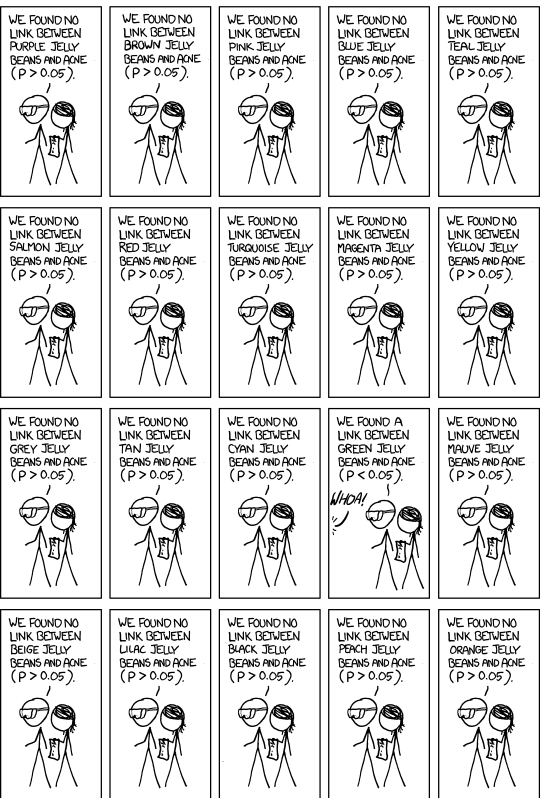
\includegraphics[height=60mm]{images/xkcd-882-grid}};
   \node[right=5mm of grid.north east,anchor=north west,text width=36mm,font=\small,align=left] {%
      Twenty colors tested at \(\alpha = 0.05\), one comes out significant, and only that one makes the news.\\[3mm]
      \textcolor{gray}{\footnotesize Comic\supercite{munroe2011significant} \link{https://xkcd.com/882/}{CC BY-NC 2.5}}};
\end{tikzpicture}
\ShowPerson{munroe}
\NoteRef{testing/twenty-jelly-beans}
\end{frame}

\begin{frame}{Multiple Testing}
\begin{tikzpicture}[
   Test/.style={circle,draw=SoftGray,fill=BackGray,minimum size=6mm,inner sep=0pt,font=\tiny},
   Hit/.style={Test,draw=Warn,fill=Warn!25,font=\tiny\sbseries},
]
   \foreach \i in {0,...,19} {
      \pgfmathtruncatemacro\col{mod(\i,5)}
      \pgfmathtruncatemacro\row{div(\i,5)}
      \node[Test] (t\i) at (\col*8mm,-\row*8mm) {};
   }
   \node[above=3mm,font=\small,align=center] at($(t0.north)!.5!(t4.north)$) {20 true null hypotheses, \(\alpha = 0.05\)};
   \onslide<2->{\node[Hit] at(t13) {.03};}
   \node[right=12mm,anchor=north west,text width=6.8cm,font=\footnotesize,align=left,visible on=<3->] (chance) at([yshift=4mm]t4.north east) {%
      Chance of at least one false positive\\(for independent tests):\\
      \(1 - (1 - 0.05)^{20} \approx \mrValueOf{round(1 - 0.95^20, 2)}\)};
   \node[below=2mm of chance.south west,anchor=north west,text width=6.8cm,font=\footnotesize,align=left,visible on=<4->] (bonferroni) {%
      \textsb{Bonferroni}: test each at \(\alpha / m = 0.05 / 20 = 0.0025\).\supercite{dunn1961multiple}
      This keeps the family-wise error rate at most \(\alpha\), at the cost of power.};
\end{tikzpicture}
\ShowPerson{bonferroni}
\Stage[14mm]{Model}
\NoteRef{testing/multiple-testing}
\end{frame}


\begin{frame}[label=plot-multiple-tests]{Correcting for Many Tests}
\centering
\begin{tikzpicture}
   \node[Plot] (plot) at (0,0) {\includegraphics[width=6.6cm]{multiple-tests}};
   \node[right=6mm,anchor=north west,text width=5.6cm,font=\small,align=left] (fwer) at(plot.north east) {%
      \textsb{Hardly ever a single false positive}\\
      \textcolor{gray}{\footnotesize family-wise error rate (FWER)}\\[1mm]
      \textsb{Holm}:\supercite{holm1979sequential} sort the \(p\)-values, compare with \(\alpha/m\), \(\alpha/(m-1)\), \dots, and stop at the first miss. At least as powerful as Bonferroni\supercite{dunn1961multiple}};
   \node[below=4mm of fwer.south west,anchor=north west,text width=5.6cm,font=\small,align=left,visible on=<2->] (fdr) {%
      \textsb{Few false positives among many findings}\\
      \textcolor{gray}{\footnotesize false discovery rate (FDR)}\\[1mm]
      \textsb{Benjamini--Hochberg}:\supercite{benjamini1995fdr} compare the \(k\)-th smallest \(p\) with \(k\alpha/m\). Everything up to the last hit counts};
   \node[below=3mm of plot.south west,anchor=north west,text width=6.4cm,font=\footnotesize,visible on=<3->] {%
      \bR{p.adjust(}\NotShown{pvals}{p}\kern-.25em\bR{, method = "holm")}\\\bR{p.adjust(}\NotShown{pvalsb}{p}\kern-.25em\bR{, method = "BH")}\\[.5mm]\textcolor{gray}{\texttt{p}: all your \(p\)-values}};
\end{tikzpicture}
\PlotCode{multiple-tests}
\Stage{Model}
\NoteRef{testing/plot-multiple-tests}
\NoteBoard{\begin{tabular}{@{}lccccl@{}}
   sorted \(p\)-values, \(m = 4\) & 0.001 & 0.015 & 0.030 & 0.040 & \\
   Bonferroni, always \(0.05/4\) & \BoardHit{0.0125} & 0.0125 & 0.0125 & 0.0125 & 1 significant\\
   Holm, \(0.05/4\), \(0.05/3\), \dots & \BoardHit{0.0125} & \BoardHit{0.0167} & 0.025 & stop & 2 significant\\
   Benjamini--Hochberg, \(k \cdot 0.05/4\) & \BoardHit{0.0125} & \BoardHit{0.025} & \BoardHit{0.0375} & \BoardHit{0.05} & 4 significant
\end{tabular}}
\end{frame}

\begin{frame}{The Garden of Forking Paths}
\begin{tikzpicture}[
   Choice/.style={Pill=BaseGray!70,font=\scriptsize\sbseries},
   Leaf/.style={font=\scriptsize,text=gray,inner sep=2pt,text height=1.6ex,text depth=.45ex},
   Lucky/.style={Pill=Warn,font=\scriptsize\sbseries,inner sep=2pt},
   level distance=15mm,
   level 1/.style={sibling distance=42mm},
   level 2/.style={sibling distance=21mm},
   level 3/.style={sibling distance=10.5mm},
   edge from parent path={(\tikzparentnode.south) -- ++(0,-4mm) -| (\tikzchildnode.north)},
   edge from parent/.style={draw,SoftGray,thick,rounded corners=3pt},
   grow=down,
]
   \node[Choice] (root) {raw data}
      child {node[Choice] {all rows}
         child {node[Choice] {raw}
            child {node[Leaf] {.21}}
            child {node[Leaf] {.34}}}
         child {node[Choice] {log}
            child {node[Leaf] {.12}}
            child {node[Leaf] {.08}}}}
      child {node[Choice] {no outliers}
         child {node[Choice] {raw}
            child {node[Leaf] {.09}}
            child {node[Leaf] {.06}}}
         child {node[Choice] {log}
            child {node[Leaf] {.11}}
            child {node[Lucky,visible on=<2->] (lucky) {.04}}}};
   \node[below=.5mm,font=\tiny\sbseries,text=Warn,visible on=<2->] at(lucky.south) {published};
   \foreach \level/\what in {1/subset,2/transform,3/{test: \(p\)}} \node[anchor=east,font=\scriptsize,gray] at(-4.4,-\level*15mm) {\what};
   \node[right=7mm,anchor=north west,text width=4cm,font=\small,align=left,visible on=<3->] (hack) at([yshift=2mm]root.north -| lucky.east) {%
      \textsb{\(p\)-hacking}: trying analyses until one is significant.\supercite{simmons2011falsepositive,head2015phacking}};
   \node[below=2.5mm of hack.south west,anchor=north west,text width=4cm,font=\small,align=left,visible on=<4->] (hark) {%
      \textsb{HARKing}: hypothesizing after the results.\supercite{kerr1998harking}};
   \node[below=2.5mm of hark.south west,anchor=north west,text width=4cm,font=\small,align=left,visible on=<5->] (fork) {%
      Each data-driven choice could go another way.\supercite{gelman2014forking}};
   \node[below=2.5mm of fork.south west,anchor=north west,text width=4cm,font=\small,align=left,visible on=<6->] {%
      \textcolor{plotblue}{\sbseries Remedies}: preregister, script, report all.\supercite{munafo2017manifesto}};
\end{tikzpicture}
\KeyMessage<6->{Write down the analysis before you see the results, and report all of it.}
\ShowPerson{borges}
\Stage[14mm]{Model,Communicate}
\NoteRef{testing/the-garden-of-forking-paths}
\end{frame}

\begin{frame}[label=plot-benchmark,optional]{Benchmarking a Tool}
Compare the simulated run times of two tools, A and B, on the same input:\supercite{berger2018checklist,ralph2021standards}\\[2mm]
\begin{columns}[c,onlytextwidth]
   \begin{column}{.42\textwidth}
      \centering
      \begin{tikzpicture}
         \node[Plot] (plot) {\includegraphics[width=5cm]{benchmark-1}};
         \node[below=1mm,Note,font=\small] at(plot.south) {one process of tool A};
      \end{tikzpicture}
   \end{column}
   \begin{column}{.54\textwidth}
      \small
      \begin{itemize}
         \item<2-> Repeat: fresh processes, several runs each\supercite{kalibera2013rigorous}
         \item<3-> Discard the warm-up, check for a steady state\supercite{barrett2017warmup}
         \item<4-> Quiet machine: no load, fixed CPU frequency
      \end{itemize}
   \end{column}
\end{columns}
\PinguSays<5->{Even the link order can shift run times by percents!\supercite{mytkowicz2009wrong}}
\PlotCode{benchmark}
\Stage{Model}
\NoteRef{testing/plot-benchmark}
\end{frame}

\begin{frame}[fragile,label=comparing-tools,optional]{Comparing Two Tools}
\begin{columns}[c,onlytextwidth]
   \begin{column}{.3\textwidth}
      \centering
      \begin{tikzpicture}
         \node[Plot] (plot) {\includegraphics[width=3.4cm]{benchmark-2}};
         \node[below=1mm,Note,font=\small,text width=3.6cm,align=center] at(plot.south) {one point per process};
      \end{tikzpicture}
   \end{column}
   \begin{column}{.66\textwidth}
\footnotesize
\begin{minted}[escapeinside={!*}{*!},mrprefix={library(dplyr); library(tidyr); set.seed(7); runs <- expand_grid(tool = c('A', 'B'), process = 1:10, iteration = 1:30) |> mutate(level = rep(rnorm(20, 0, 3), each = 30), time = ifelse(tool == 'A', 100, 94) + level + 60 * exp(-(iteration - 1) / 3) + rnorm(n(), 0, 1.5)); steady <- runs |> filter(iteration > 10) |> summarize(time = mean(time), .by = c(tool, process))}]{R}
a <- !*\textcolor{NotShownGray}{steady}\NotShownAfter{steady}{steady}*!$time[!*\textcolor{NotShownGray}{steady}\NotShownAfter{steadyb}{steady}*!$tool == "A"]
b <- !*\textcolor{NotShownGray}{steady}\NotShownAfter{steadyc}{steady}*!$time[!*\textcolor{NotShownGray}{steady}\NotShownAfter{steadyd}{steady}*!$tool == "B"]
median(b) / median(a)     # 0.96: here B needs 4 % less
wilcox.test(a, b)$p.value # 0.035
mean(outer(a, b, ">"))    # A12 = 0.78: A slower
\end{minted}
      \small
      \begin{itemize}
         \item<2-> \textsb{One value per process}: runs inside a process depend on each other, so average them first\supercite{georges2007rigorous}
         \item<3-> \textsb{Ranks} for skewed run times: \bR{wilcox.test()} and \(\hat A_{12}\)\supercite{arcuri2014hitchhiker,vargha2000critique}\\
            {\footnotesize\color{gray}\(\hat A_{12}\): the chance that a process of A is slower than one of B; 0.5: neither tends to win}
      \end{itemize}
   \end{column}
\end{columns}
\VarNote[north]{ns-steady}{(34mm,3mm)}{one row per process}
\PlotCode{benchmark}
\KeyMessage<4->{Report how much faster, and how often.\supercite{berger2018checklist,ralph2021standards}}
\Stage{Model,Communicate}
\NoteRef{testing/comparing-tools}
\end{frame}

% the urls contain slashes, so the \foreach list names them by key
\csdef{check@sigplan}{https://www.sigplan.org/Resources/EmpiricalEvaluation/}
\csdef{check@sigsoft}{https://www2.sigsoft.org/EmpiricalStandards/}
\csdef{check@hoefler}{https://doi.org/10.1145/2807591.2807644}
\csdef{check@artifacts}{https://www.acm.org/publications/policies/artifact-review-and-badging-current}
\begin{frame}{Checklists for Empirical Evaluations}
\centering
\vspace*{4mm}
\begin{tikzpicture}[
   Gallery/.style={Card,align=center,text width=26mm,anchor=north,font=\scriptsize},
]
   \foreach[count=\i] \key/\name/\what in {
      sigplan/SIGPLAN Guidelines\supercite{berger2018checklist}/{claims, baselines, benchmarks, analysis, presentation},
      sigsoft/SIGSOFT Empirical Standards\supercite{ralph2021standards}/{what reviewers expect, per kind of study},
      hoefler/Twelve Rules\supercite{hoefler2015benchmarking}/{for reporting performance results},
      artifacts/Artifact Evaluation/{badges for available, functional, and reproduced artifacts}%
   } {
      \node[Gallery,visible on=<\i->,href node=\csuse{check@\key}] at({(\i-1)*32mm},0)
         {\Qr[PartTint]{19mm}{\csuse{check@\key}}\\[2mm]\parbox[t][7mm][t]{26mm}{\centering\textsb{\name}}\\[1mm]
          \parbox[t][11mm][t]{26mm}{\centering\textcolor{gray}{\what}}};
   }
\end{tikzpicture}
\KeyMessage<5->{Always consult checklists!}
\NoteRef{testing/checklists-for-empirical-evaluations}
\end{frame}

\NextNoteRef{testing/takeaways-1}
\Takeaways[Testing]{
   \Learning{check-square-o}{Plan the test and \(n\) first}{Decided after seeing \(p\)? Fine, but report it as exploratory.}
   \Learning{arrows-h}{Report effect, interval, and \(n\)}{How large, how certain, from how much data, and what it means.}
   \Learning{percent}{Read \(p\) correctly}{It is not the chance that \(H_0\) is true. It says how surprising the data would be without an effect.}
   \Learning{code-fork}{Count every test}{Many tests make false hits likely. Correct with Holm, report all.}
}

\Chapter{3}

\begin{frame}[label=plot-communicate,optional]{Communicating With Graphs}
\centering
\vspace*{3mm}
\begin{tikzpicture}
   \node[Plot] (bad) at (0,0) {\includegraphics[width=4.6cm]{communicate-1}};
   \node[Plot,right=16mm of bad,visible on=<2->] (good) {\includegraphics[width=4.6cm]{communicate-2}};
   \node[below=1mm,Note,font=\small] at(bad.south) {default: legend, no message};
   \node[below=1mm,Note,font=\small,visible on=<2->] at(good.south) {means with intervals, labels, the message as title};
\end{tikzpicture}
\KeyMessage<3->{Put the message in the title, and label the groups directly instead of using a legend.}
\ShowPerson{nightingale}
\PlotCode{communicate}
\Stage[14mm]{Visualize,Communicate}
\NoteRef{communicating/plot-communicate}
\end{frame}

\begin{frame}[optional]{Three Laws of Communication}
\centering
{\small\color{gray}after Jean-luc Doumont\supercite{doumont2002laws}\par}\vspace{3mm}
\begin{tikzpicture}[Law/.style={Card,anchor=north west,text width=37mm,font=\small,align=left,minimum height=40mm}]
   \foreach[count=\i] \law/\plot in {
      {Adapt to your audience}/{A slide needs larger text and fewer details than a figure in a paper.},
      {Maximize the signal-to-noise ratio}/{Remove what does not carry data: frames, heavy grids, 3D effects, decoration.},
      {Use effective redundancy}/{Say the message twice: in the title and in the plot, by color and by label.}%
   } {
      \node[Law,draw=PartTint,visible on=<\i->] at ({(\i-1)*44mm},0) {\textsb{\i. \law}\\[2mm]\plot};
   }
\end{tikzpicture}
\KeyMessage<4->{You should be able to say in one sentence what each plot shows.\supercite{doumont2009trees,tufte2001visual}}
\Stage{Communicate}
\NoteRef{communicating/three-laws-of-communication}
\end{frame}

% a row of the ladder of encodings, the same height for every picture
\newcommand\Row[1]{\parbox[c][6.5mm][c]{24mm}{\centering #1}}
\begin{frame}[label=plot-pie-bar]{Visual Encodings}
\centering
\begin{tikzpicture}
   \node[anchor=north west,font=\small] (ladder) at (0,0) {%
      \renewcommand\arraystretch{1}%
      \begin{tabular}{@{}c@{\quad}l@{\quad}c@{}}
         \onslide<2->{\textsb{1} & Position on a common scale & \Row{\GlyphPosition}} \\
         \onslide<3->{\textsb{2} & Position on non-aligned scales & \Row{\GlyphAligned}} \\
         \onslide<4->{\textsb{3} & Length, direction, angle & \Row{\GlyphLength\,\GlyphAngle}} \\
         \onslide<5->{\textsb{4} & Area & \Row{\GlyphArea}} \\
         \onslide<6->{\textsb{5} & Volume, curvature & \Row{\GlyphVolume\,\GlyphCurvature}} \\
         \onslide<7->{\textsb{6} & Shading, color saturation & \Row{\GlyphShade}}
      \end{tabular}%
   };
   \node[above right,yshift=1.5mm,font=\small\sbseries] at(ladder.north west) {How accurately we read values\supercite{cleveland1984graphical}};
   \onslide<2->{\draw[Link,gray,thick] ([xshift=-3mm,yshift=-4mm]ladder.north west) -- ([xshift=-3mm,yshift=4mm]ladder.south west) node[midway,left,rotate=90,anchor=south,font=\tiny,gray] {less accurate};}

   \onslide<8->{
      \node[Plot,anchor=north west] (pie) at ([xshift=5mm,yshift=-2mm]ladder.north east) {\includegraphics[width=2.4cm]{pie-chart}};
      \node[above,yshift=1.5mm,font=\small\sbseries] at(pie.north) {Which slice is bigger, C or D?};
   }
   \onslide<9->{
      \node[Plot,right=2mm of pie.north east,anchor=north west] (bar) {\includegraphics[width=2.5cm]{bar-chart}};
   }
\end{tikzpicture}
\KeyMessage<10->{Put the comparison you care about most on a shared axis.}
\PlotCode{pie-bar}
\Stage{Visualize}
\NoteRef{communicating/plot-pie-bar}
\end{frame}

% tiny sketches of the charts: x from 0 to 10, y from 0 to 10
\newcommand\ChartIcon[1]{\tikz[x=.48mm,y=.26mm,baseline=.2mm,sharp corners,line width=.3pt,plotblue]{\path (0,0) rectangle (10,10);#1}}
\newcommand\IconHist{\foreach \x/\h in {0/3,2/6,4/10,6/7,8/3}{\fill (\x,0) rectangle ++(1.8,\h);}}
\newcommand\IconDens{\fill plot[smooth,domain=0:10,samples=20] (\x,{10*exp(-(\x-5)^2/5)}) -- (10,0) -- (0,0) -- cycle;}
\newcommand\IconBox{\draw (0,5) -- (10,5);\filldraw[fill=white] (3,2) rectangle (7,8);\draw (5,2) -- (5,8);}
\newcommand\IconScat{\foreach \x/\y in {1/2,2/4,3/3,4/6,5/4,6/7,7/6,8/8,9/9}{\fill (\x,\y) circle[radius=.5];}}
\newcommand\IconTwod{\draw (5,5) ellipse[x radius=5,y radius=5];\draw (5,5) ellipse[x radius=3,y radius=3];\fill (5,5) ellipse[x radius=1.2,y radius=1.2];}
\newcommand\IconHex{\foreach \x/\y/\o in {2/3/40,5/3/100,8/3/60,3.5/7.5/80,6.5/7.5/30}{\fill[plotblue!\o] (\x+1.5,\y) -- (\x+.75,\y+2.2) -- (\x-.75,\y+2.2) -- (\x-1.5,\y) -- (\x-.75,\y-2.2) -- (\x+.75,\y-2.2) -- cycle;}}
\newcommand\IconBar{\foreach \x/\h in {.5/9,4/6,7.5/3}{\fill (\x,0) rectangle ++(2,\h);}}
\newcommand\IconLol{\foreach \x/\h in {1.5/9,5/6,8.5/3}{\draw (\x,0) -- (\x,\h);\fill (\x,\h) circle[radius=.9];}}
\newcommand\IconTree{\draw (0,0) rectangle (10,10) (6,0) -- (6,10) (0,4) -- (6,4) (6,6) -- (10,6);\fill (0,4) rectangle (6,10);}
\newcommand\IconGbox{\foreach \x/\l/\h in {1/2/6,6/4/9}{\draw (\x+1.5,0) -- (\x+1.5,10);\filldraw[fill=white] (\x,\l) rectangle ++(3,\h-\l);\draw (\x,{(\l+\h)/2}) -- ++(3,0);}}
\newcommand\IconVio{\foreach \c in {2.5,7.5}{\fill plot[smooth,variable=\t,domain=0:10,samples=12] ({\c+2*exp(-(\t-5)^2/6)},\t) -- plot[smooth,variable=\t,domain=10:0,samples=12] ({\c-2*exp(-(\t-5)^2/6)},\t) -- cycle;}}
\newcommand\IconRidge{\foreach \b/\m in {5/4,0/6}{\filldraw[fill=white] plot[smooth,domain=0:10,samples=15] (\x,{\b+5*exp(-(\x-\m)^2/3)}) -- cycle;}}
\newcommand\IconLine{\draw (0,2) -- (2.5,5) -- (5,4) -- (7.5,8) -- (10,7);}
\newcommand\IconArea{\fill (0,0) -- (0,2) -- (2.5,5) -- (5,4) -- (7.5,8) -- (10,7) -- (10,0) -- cycle;}
\newcommand\IconSmall{\foreach \x in {0,3.6,7.2}{\draw[gray,line width=.2pt] (\x,0) rectangle ++(2.8,10);\draw (\x,2) -- ++(1.4,5) -- ++(1.4,-2);}}
\begin{frame}{Choosing a Chart}
\begin{tikzpicture}[
   Kind/.style={Pill=plotblue!80,font=\scriptsize\sbseries,minimum width=23mm,text height=1.6ex,text depth=.4ex},
   Chart/.style={font=\footnotesize,anchor=west,inner sep=1pt,text height=1.6ex,text depth=.4ex},
   level distance=13mm,
   level 1/.style={sibling distance=29mm,
      edge from parent path={(\tikzparentnode.south) -- ([yshift=-3mm]\tikzparentnode.south) -| (\tikzchildnode.north)},
      edge from parent/.style={draw,SoftGray,thick,rounded corners=3pt}},
   level 2/.style={
      grow via three points={one child at (-6.5mm,-8mm) and two children at (-6.5mm,-8mm) and (-6.5mm,-13.5mm)},
      edge from parent path={([xshift=-9mm]\tikzparentnode.south) |- (\tikzchildnode.west)},
      edge from parent/.style={draw,SoftGray,rounded corners=3pt},
   },
]
   \node[Pill=BaseGray,font=\small\sbseries,inner xsep=8pt,inner ysep=4pt] (data) {What kind of data do you have?}
      child[visible on=<2->] {node[Kind] {\faBarChart~One numeric}
         child {node[Chart] {\ChartIcon{\IconHist}~histogram}} child {node[Chart] {\ChartIcon{\IconDens}~density}} child {node[Chart] {\ChartIcon{\IconBox}~boxplot}}}
      child[visible on=<3->] {node[Kind] {\faCrosshairs~Two numeric}
         child {node[Chart] {\ChartIcon{\IconScat}~scatter}} child {node[Chart] {\ChartIcon{\IconTwod}~2D density}} child {node[Chart] {\ChartIcon{\IconHex}~hexbin}}}
      child[visible on=<4->,edge from parent path={(\tikzparentnode.south) -- (\tikzchildnode.north)}] {node[Kind] {\faTags~Categorical}
         child {node[Chart] {\ChartIcon{\IconBar}~barplot}} child {node[Chart] {\ChartIcon{\IconLol}~lollipop}} child {node[Chart] {\ChartIcon{\IconTree}~treemap}}}
      child[visible on=<5->] {node[Kind] {\faSliders~Num \& Cat}
         child {node[Chart] {\ChartIcon{\IconGbox}~grouped box}} child {node[Chart] {\ChartIcon{\IconVio}~violin}} child {node[Chart] {\ChartIcon{\IconRidge}~ridgeline}}}
      child[visible on=<6->] {node[Kind] {\faLineChart~Time series}
         child {node[Chart] {\ChartIcon{\IconLine}~line}} child {node[Chart] {\ChartIcon{\IconArea}~area}} child {node[Chart] {\ChartIcon{\IconSmall}~small multiples}}};
   \node[below=38mm,font=\small,gray,visible on=<7->] at(data.south) {Simple usually beats fancy: AI can generate impressive plots in seconds that mean nothing};
\end{tikzpicture}
\KeyMessage<8->{Pick the chart from the data type, then read its caveats.\supercite{holtz2018datatoviz}}
\Tutorial{https://www.data-to-viz.com/}{data-to-viz.com: the full decision tree}
\Stage{Visualize}
\NoteRef{communicating/choosing-a-chart}
\end{frame}

\begin{frame}[label=plot-overplotting,optional]{Overplotting}
\centering
\begin{tikzpicture}
   \node[Plot] (p1) at (0,0) {\includegraphics[width=4.1cm]{overplot-1}};
   \node[Plot,right=4mm of p1,visible on=<2->] (p2) {\includegraphics[width=4.1cm]{overplot-2}};
   \node[Plot,right=4mm of p2,visible on=<3->] (p3) {\includegraphics[width=4.1cm]{overplot-3}};
   \node[below=1mm,Note] at(p1.south) {\bR{geom_point()}: a black blob};
   \node[below=1mm,Note,visible on=<2->] at(p2.south) {transparency shows density};
   \node[below=1mm,Note,visible on=<3->] at(p3.south) {hexagonal binning counts points per cell};
\end{tikzpicture}
\PlotCode{overplotting}
\KeyMessage<4->{With \mrValueOf{format(nrow(ggplot2::diamonds), big.mark = ",")} points, show the density, not the points.\supercite{holtz2018datatovizcaveats}}
\Stage{Visualize}
\NoteRef{communicating/plot-overplotting}
\end{frame}

\begin{frame}[label=plot-spaghetti]{Spaghetti Plots}
\centering
\begin{tikzpicture}
   \node[Plot] (p1) at (0,0) {\includegraphics[width=5.3cm]{spaghetti-1}};
   \node[Plot,right=8mm of p1,visible on=<2->] (p2) {\includegraphics[width=5.3cm]{spaghetti-2}};
   \node[below=1mm,Note,font=\small] at(p1.south) {50 chicks, 50 colors, no story};
   \node[below=1mm,Note,font=\small,visible on=<2->] at(p2.south) {small multiples and one highlighted summary};
\end{tikzpicture}
\ShowPerson{tufte}
\PlotCode{spaghetti}
\KeyMessage<3->{Split by a grouping variable, gray out the context, and highlight what matters.\supercite{holtz2018datatovizcaveats}}
\Stage[14mm]{Visualize}
\NoteRef{communicating/plot-spaghetti}
\end{frame}

\begin{frame}[label=plot-colours]{Color Scales}
\centering
\begin{tikzpicture}
   \node[Plot] (rainbow) at (0,0) {\includegraphics[width=2.9cm]{volcano-rainbow}};
   \node[Plot,right=2mm of rainbow,visible on=<2->] (viridis) {\includegraphics[width=2.9cm]{volcano-viridis}};
   \node[Plot,right=8mm of viridis,visible on=<3->] (rainbow-grey) {\includegraphics[width=2.9cm]{volcano-rainbow-grey}};
   \node[Plot,right=2mm of rainbow-grey,visible on=<3->] (viridis-grey) {\includegraphics[width=2.9cm]{volcano-viridis-grey}};
   \foreach \n/\t/\o in {rainbow/Rainbow/1,viridis/Viridis/2,rainbow-grey/Rainbow in gray/3,viridis-grey/Viridis in gray/3}
      \node[above=1mm,font=\small\sbseries,visible on=<\o->] at(\n.north) {\t};
\end{tikzpicture}
\PlotCode{colours}
\KeyMessage<4->{The rainbow invents edges and loses its order in gray: use viridis\supercite{garnier2024viridis} or ColorBrewer.\supercite{harrower2003colorbrewer}}
\Stage{Visualize}
\NoteRef{communicating/plot-colours}
\end{frame}

\begin{frame}[label=plot-color-vision,optional]{Color Vision Deficiency}
\centering
\begin{tikzpicture}
   \node[Plot] (plot) at (0,0) {\includegraphics[width=11.5cm]{color-vision}};
   \node[below=2mm,font=\small,text width=11.5cm,align=center] at(plot.south) {%
      About \qty{8}{\percent} of men have a red-green deficiency.\supercite{birch2012prevalence} The rainbow loses its order for them, viridis keeps it.\supercite{garnier2024viridis}};
\end{tikzpicture}
\PlotCode{color-vision}
\ShowPerson{dalton}
\Stage[14mm]{Visualize}
\NoteRef{communicating/plot-color-vision}
\end{frame}

\begin{frame}[label=plot-encode-twice]{Encode Twice}
\centering
\begin{tikzpicture}
   \node[Plot] (one) at (0,0) {\includegraphics[width=5cm]{encode-twice-1}};
   \node[Plot,right=10mm of one,visible on=<2->] (two) {\includegraphics[width=5cm]{encode-twice-2}};
   \node[below=1mm,Note,font=\small] at(one.south) {color alone, legend far away};
   \node[below=1mm,Note,font=\small,visible on=<2->] at(two.south) {color, shape, and a direct label};
\end{tikzpicture}
\PlotCode{encode-twice}
\KeyMessage<3->{Color alone fails in gray print and for about 1 in 12 men: add a shape, a label, or a position.}
\Stage{Visualize,Communicate}
\NoteRef{communicating/plot-encode-twice}
\end{frame}

% the urls contain slashes, so the \foreach list names them by key
\csdef{gallery@datatoviz}{https://www.data-to-viz.com}
\csdef{gallery@rgallery}{https://r-graph-gallery.com}
\csdef{gallery@ftvocabulary}{https://github.com/Financial-Times/chart-doctor}
\csdef{gallery@vizcatalogue}{https://datavizcatalogue.com}
\csdef{gallery@vizproject}{https://datavizproject.com}
\begin{frame}{Chart Catalogues}
\centering
\vspace*{4mm}
\begin{tikzpicture}[
   Gallery/.style={Card,align=center,text width=21mm,anchor=north,font=\scriptsize},
]
   \foreach[count=\i] \key/\name/\what in {
      datatoviz/From Data to Viz/{a decision tree from the data type},
      rgallery/R Graph Gallery/{hundreds of plots with R code},
      ftvocabulary/FT Visual Vocabulary/{charts by the relation they show},
      vizcatalogue/Data Viz Catalogue/{what each chart can and cannot do},
      vizproject/Data Viz Project/{charts by function and shape}%
   } {
      % five shades from the first to the last part color; fixed text heights keep the codes in one row
      \pgfmathtruncatemacro\mix{100-(\i-1)*25}
      \colorlet{gallery}{PartOne!\mix!PartFour}
      \node[Gallery,draw=gallery!60,visible on=<\i->,href node=\csuse{gallery@\key}] at({(\i-1)*27.5mm},0)
         {\Qr[gallery]{19mm}{\csuse{gallery@\key}}\\[2mm]\parbox[t][7mm][t]{21mm}{\centering\textsb{\name}}\\[1mm]
          \parbox[t][11mm][t]{21mm}{\centering\textcolor{gray}{\what}}};
   }
\end{tikzpicture}
\Stage{Visualize}
\NoteRef{communicating/chart-catalogues}
\end{frame}

\Chapter{4}

\begin{frame}{What Is Being Measured?}
\centering
\begin{tikzpicture}[x=1.25cm,
   Stop/.style={circle,draw=BaseGray,fill=white,thick,minimum size=5mm,inner sep=0pt,font=\scriptsize\sbseries},
   OnTime/.style={Stop,fill=plotblue!20,draw=plotblue},
   Late/.style={Stop,fill=Warn!20,draw=Warn},
   Gone/.style={Stop,dashed,draw=gray,text=gray},
   Delay/.style={below=2mm,font=\scriptsize,align=center},
]
   \draw[SoftGray,line width=2pt,line cap=round] (0,0) -- (10,0);
   \foreach \x/\name in {0/A,10/D} \node[Stop] (\name) at (\x,0) {\name};
   \node[Stop] (B) at (10/3,0) {B};
   \node[Stop] (C) at (20/3,0) {C};
   \onslide<2->{
      \node[OnTime] at(A) {A};
      \node[Delay] at(A.south) {\(+2\) min\\on time};
   }
   \onslide<3->{
      \node[Late] at(B) {B};
      \node[Delay] at(B.south) {\(+9\) min\\late};
   }
   \onslide<4->{
      \node[Gone] at(C) {C};
      \node[Delay,gray] at(C.south) {cancelled};
   }
   \onslide<5->{
      \node[OnTime] at(D) {D};
      \node[Delay] at(D.south) {\(+3\) min\\on time};
   }
   \node[above=3mm,font=\small,align=center] at(5,0) {A made-up train with four planned stops. On time means less than six minutes late.\supercite{kriesel2019bahnmining}};

   \node[Card,below=18mm,anchor=north east,text width=50mm,font=\small,visible on=<6->] (db) at(4.6,0) {%
      \textsb{Only stops that happened}\\[1mm]
      2 of 3 on time: \qty{67}{\percent}};
   \node[Card,below=18mm,anchor=north west,text width=50mm,font=\small,visible on=<7->] (all) at(5.4,0) {%
      \textsb{All planned stops}\\[1mm]
      2 of 4 on time: \qty{50}{\percent}};
\end{tikzpicture}
\KeyMessage<8->{Cancelled trains are not counted, so cancelling a late train improves the rate. Ask what is missing from the denominator.}
\Stage{Communicate}
\NoteRef{communicating/what-is-being-measured}
\end{frame}

\begin{frame}{Twice as Fast?}
\begin{tikzpicture}[
   /pgfplots/Runtime/.style={lecture axis,ybar,bar width=10mm,width=4.6cm,height=5cm,
      symbolic x coords={ours,theirs},xtick=data,enlarge x limits=.5,ymax=45,
      ylabel={Runtime (s)},nodes near coords,every node near coord/.append style={font=\scriptsize},
      title style={font=\scriptsize\sbseries}},
]
   \begin{axis}[Runtime,name=cut,ymin=38,title={\textcolor{Warn}{\enquote{We are twice as fast!}}}]
      \RoundBars[fill=plotblue!70]{38}{(ours,40) (theirs,42)}
   \end{axis}
   \begin{scope}[visible on=<2->]
   \begin{axis}[Runtime,name=full,at={(cut.south east)},anchor=south west,xshift=12mm,ymin=0,title={The same runtimes from zero}]
      \RoundBars[fill=plotblue!70]{0}{(ours,40) (theirs,42)}
   \end{axis}
   \end{scope}
   \node[right=8mm,anchor=north west,text width=4.4cm,font=\small,align=left,visible on=<3->] at(full.north east) {%
      The axis starts at \qty{38}{\second}.\\ The bars are \(2\) and \(4\) long.\\[2mm]
      The real ratio: \(42 / 40 = 1.05\).\\ Five percent, not twice.\supercite{huff1954lie}\\[2mm]\textcolor{gray}{\footnotesize Run time is on a ratio scale: it has a true zero, so \enquote{twice} needs that zero.}};
\end{tikzpicture}
\KeyMessage<4->{\enquote{Twice}, \enquote{half}, \enquote{\qty{+50}{\percent}} are ratios: their axis must start at zero.\\ Better yet, state the ratio itself.}
\Stage{Visualize,Communicate}
\NoteRef{communicating/twice-as-fast}
\end{frame}

\begin{frame}{Axes and Baselines}
\alt<1|handout:0>{\def\AxisMin{74.5}\def\AxisMax{76.8}}{\def\AxisMin{0}\def\AxisMax{100}}
\begin{tikzpicture}
   \begin{axis}[
      lecture axis,
      ybar,
      bar width=14mm,
      width=7cm,height=5.4cm,
      symbolic x coords={Goal 2019,Reached 2018},
      xtick=data,
      enlarge x limits=.45,
      ymin=\AxisMin,ymax=\AxisMax,
      ylabel={Punctual long-distance trains (\%)},
      nodes near coords,
      every node near coord/.append style={font=\scriptsize},
      name=bars,
   ]
      \RoundBars[fill=plotblue!70]{\AxisMin}{(Goal 2019,76.5) (Reached 2018,74.9)}
   \end{axis}
   \node[right=8mm,anchor=north west,text width=5.4cm,font=\small,align=left] (story) at(bars.north east) {%
      \alt<1|handout:0>{An axis starting at \qty{74.5}{\percent}: a dramatic gap.}{The same two numbers from zero: \num{1.6} percentage points apart.}\\[1mm]
      {\scriptsize\color{gray}Numbers: Deutsche Bahn, via David Kriesel\supercite{kriesel2019bahnmining}}};
   \node[below=3mm of story.south west,anchor=north west,text width=5.4cm,font=\small,align=left,visible on=<3->] {%
      Bars encode length, so they must start at zero. Points and lines may zoom in, but mark it.\supercite{huff1954lie,cairo2019charts}};
\end{tikzpicture}
\Stage{Visualize,Communicate}
\NoteRef{communicating/axes-and-baselines}
\end{frame}

\begin{frame}{Relative or Absolute?}
\centering
\begin{tikzpicture}
   % 1995: the risk of a thrombosis \enquote{doubled} with a newer pill
   \node[anchor=north west,text width=58mm,font=\normalsize\sbseries,align=left,inner sep=0pt] (head) at (0,0)
      {The new pill doubles the risk of thrombosis};
   \node[below=4mm of head.south west,anchor=north west,font=\small,inner sep=0pt,visible on=<2->] (rel)
      {\textsb{Relative:} \qty{+100}{\percent}};
   \node[below=2mm of rel.south west,anchor=north west,font=\small,inner sep=0pt,visible on=<3->] (claim)
      {\textsb{Absolute:} from 1 to 2 in \num{7000} women};
   \node[below=5mm of claim.south west,anchor=north west,text width=58mm,font=\footnotesize,text=darkgray,align=left,visible on=<5->] {%
      UK, 1995: many women stopped the pill.\\ About \num{13000} more abortions followed.\supercite{gigerenzer2007statistics}};
   % 7000 women as 100 x 70 dots, the cases in red
   \begin{scope}[shift={(68mm,-1mm)},visible on=<3->]
      % each row is a dashed line of 100 round dots
      \foreach \r in {0,...,69}
         \draw[SoftGray!80,line width=.34mm,line cap=round,dash pattern=on 0pt off .6mm] (0,-\r*.6mm) -- (59.5mm,-\r*.6mm);
      \fill[Warn] (31*.6mm,-24*.6mm) circle (.9mm);
      \fill[Warn,visible on=<4->] (72*.6mm,-51*.6mm) circle (.9mm);
      \node[below,font=\scriptsize,text=darkgray] at (29.7mm,-42mm) {\num{7000} women: \alt<4->{2 cases with the new pill}{1 case with the old pill}};
   \end{scope}
\end{tikzpicture}
\KeyMessage<6->{Give the absolute numbers with every relative change.\supercite{gigerenzer2007statistics}}
\ShowPerson{gigerenzer}
\Stage[22mm]{Communicate}
\NoteRef{communicating/relative-or-absolute}
\end{frame}

\begin{frame}{How Many Decimals?}
\centering
\begin{tikzpicture}
   \node[anchor=west,font=\Large,text=gray,inner sep=0pt] (bad) at (0,0) {\qty{85.71}{\percent} agree};
   \draw[Warn,thick] (bad.west) -- (bad.east);
   \node[anchor=west,font=\Large\sbseries,inner sep=0pt,visible on=<2->] (good) at([xshift=12mm]bad.east) {6 of 7 agree};
   \node[below=4mm of bad.south west,anchor=north west,font=\small,inner sep=0pt,text width=115mm,align=left,text=black] (one) {%
      \begin{itemize}
         \item<3-> One person more moves the result by 14 percentage points, so two decimals promise what 7 people cannot
         \item<4-> The \qty{95}{\percent} interval for 6 of 7 runs from \qty{42}{\percent} to \qty{99.6}{\percent}: \bR{binom.test(6, 7)}
      \end{itemize}};
\end{tikzpicture}
\KeyMessage<5->{Small samples: give the counts. Decimals only when \(n\) can carry them.}
\Stage{Communicate}
\NoteRef{communicating/how-many-decimals}
\end{frame}

\begin{frame}{Tables}
\begin{tikzpicture}
   \node[anchor=north west] (bad) at (0,0) {%
      \scriptsize\renewcommand\arraystretch{1.2}%
      \fontfamily{FiraSans-TLF}\selectfont
      \begin{tabular}{|l|l|r|r|}
         \hline
         species & sex & mass & n \\ \hline
         Adelie & female & 3368.835616 & 73 \\ \hline
         Adelie & male & 4043.493151 & 73 \\ \hline
         Chinstrap & female & 3527.205882 & 34 \\ \hline
         Chinstrap & male & 3938.970588 & 34 \\ \hline
         Gentoo & female & 4679.741379 & 58 \\ \hline
         Gentoo & male & 5484.836066 & 61 \\ \hline
      \end{tabular}%
   };
   \node[above,font=\small\sbseries,Warn] at(bad.north) {Before};
   \node[right=14mm of bad,visible on=<2->] (good) {%
      \scriptsize
      \fontfamily{FiraSans-TLF}\selectfont
      \begin{tabular}{@{}llS[table-format=4.0]S[table-format=3.0]@{}}
         \toprule
         Species & Sex & {Mean body mass (\unit{\gram})} & {\(n\)} \\
         \midrule
         Adelie & female & 3369 & 73 \\
                & male & 4043 & 73 \\
         \addlinespace
         Chinstrap & female & 3527 & 34 \\
                   & male & 3939 & 34 \\
         \addlinespace
         Gentoo & female & 4680 & 58 \\
                & male & 5485 & 61 \\
         \bottomrule
      \end{tabular}%
   };
   \node[above,font=\small\sbseries,plotblue,visible on=<2->] at(good.north) {After};
   \draw[Link,gray,thick,visible on=<2->] (bad) -- (good);
   \node[below=6mm of bad.south west,anchor=north west,text width=12.5cm,font=\small,visible on=<3->] {%
      \begin{itemize}
         \item No vertical rules, few horizontal ones\supercite{fear2020booktabs}
         \item Units in the header, numbers aligned at the decimal point
         \item Few digits. Many numbers to compare? Plot them.\supercite{gelman2002tables}
      \end{itemize}};
\end{tikzpicture}
\Stage{Communicate}
\NoteRef{communicating/tables}
\end{frame}

\begin{frame}[optional]{Figures Side by Side}
\begin{tikzpicture}[
   /pgfplots/Panel/.style={lecture axis,ybar,bar width=6mm,width=2.9cm,height=3.8cm,ymin=0,
      symbolic x coords={female,male},xtick=data,enlarge x limits=.5,title style={font=\scriptsize\sbseries}},
]
   \begin{axis}[Panel,name=a1,title={Adelie},ymax=4500,ylabel={Mean body mass (g)}]
      \RoundBars[fill=Adelie]{0}{(female,3369) (male,4043)}
   \end{axis}
   \begin{axis}[Panel,at={(a1.south east)},anchor=south west,xshift=9mm,title={Gentoo},ymax=6000]
      \RoundBars[fill=Gentoo]{0}{(female,4680) (male,5485)}
   \end{axis}
   \begin{scope}[visible on=<2->]
   \begin{axis}[Panel,name=b1,at={(a1.south east)},anchor=south west,xshift=43mm,title={Adelie},ymax=6000,ylabel={Mean body mass (g)}]
      \RoundBars[fill=Adelie]{0}{(female,3369) (male,4043)}
   \end{axis}
   \begin{axis}[Panel,at={(b1.south east)},anchor=south west,xshift=1mm,title={Gentoo},ymax=6000,yticklabels={}]
      \RoundBars[fill=Gentoo]{0}{(female,4680) (male,5485)}
   \end{axis}
   \end{scope}
   \node[below=6mm,Note,font=\small,text width=5cm,align=center] at(a1.south east) {own axes: the Adelie males look as heavy as the Gentoo males};
   \node[below=6mm,Note,font=\small,text width=5cm,align=center,visible on=<2->] at(b1.south east) {one shared axis: a position on a common scale\supercite{cleveland1984graphical}};
\end{tikzpicture}
\KeyMessage<3->{Share and align the axes of panels you compare, and keep one color per group.\\
   \bR{facet_wrap()} shares axes by default, \bR[mrpackage]{patchwork} aligns separate plots.}
\Stage{Visualize,Communicate}
\NoteRef{communicating/figures-side-by-side}
\end{frame}

\NextNoteRef{communicating/takeaways-1}
\Takeaways[Communicating]{
   \Learning{bullhorn}{Encode the message twice}{In the title and in the plot, by color and by label.}
   \Learning{eye}{Compare by encoding}{Position on a common axis reads best, then length, area, color.}
   \Learning{paint-brush}{Choose the right color palette}{Viridis keeps its order, also in gray print. Never rely on color alone.}
   \Learning{question}{Be honest with numbers}{Start ratio axes at zero, give absolute numbers, and ask what is left out.}
}


% the second lecture starts with a title page of its own, which takes no time of the timetable
\EndTiming
\date{November 10, 2026}
\maketitle[titleimage/title][20]

% \RecapAnswer{overlay}{answer}: the answer to a recap question, in gray, shown after all questions
\newcommand\RecapAnswer[2]{\onslide<#1-|handout:1>{\textcolor{darkgray}{\scriptsize\textit{#2}\endgraf}}}
\begin{frame}{Recap: Lecture 1}
   \vspace*{-3mm}
   \begin{enumerate}
      \itemsep1.5pt
      \item<2-> Why do we clean data, and what does clean data look like?\\*
         \RecapAnswer8{Typos, mixed units, and gaps carry into every test. Clean: one row per observation, one column per variable, fixed in code. Document every tidying step and keep the raw sources.}
      \item<3-> Which summary statistics can we use for an ordinal variable? Name two examples of ordinal variables.\\*
         \RecapAnswer9{Median and interquartile range, or counts. \textsb{Not} mean and standard deviation: the steps have no known size. E.\,g. agreement scales, school grades, sizes S, M, L.}
      \item<4-> What was Simpson's paradox?\\*
         \RecapAnswer{10}{A trend over all data reverses within every group, because a third variable drives both. Penguins: bill depth falls with bill length overall, but rises within each species. Group first, report per group.}
      \item<5-> Is \enquote{Our tool might be better somehow} a hypothesis?\\*
         \RecapAnswer{11}{No: better at what, and how would we see it? No result can refute \enquote{might}. Testable: \enquote{With our tool, the tasks take less time on average.}}
      \item<6-> What does a \(t\)-test measure?\\*
         \RecapAnswer{12}{Whether two means differ by more than noise explains: \(t\) is the difference of the means divided by its standard error. Report it with \(n\), the difference and its \qty{95}{\percent} confidence interval, \(t\), degrees of freedom, exact~\(p\).}
      \item<7-> What does \(p = 0.03\) tell you, and why is \(p\) alone not enough?\\*
         \RecapAnswer{13}{How surprising our data would be under \(H_0\), not the chance that \(H_0\) is true. Alone it misleads: \textsb{p-hacking}, \textsb{no effect size}, tiny effects significant with large \(n\), 0.05 is arbitrary.\supercite{wasserstein2016asa}}
   \end{enumerate}
\NoteRef{main/lecture-1-in-one-slide}
\end{frame}

\StartTiming{talk1}
% The results paragraph of the talk group with planted flaws, and their fixes: shared by the slides and by
% report-flaws.tex, the clickable version to present
% \BadReport: a results paragraph with planted flaws. \Flaw{n}{text} marks a flaw, \Good{text} something done right;
% both are plain text in the task and marked in the answer
\colorlet{GoodGreen}{green!40!black}
\newcommand\Flaw[2]{#2}
\newcommand\Good[1]{#1}
% how bad each flaw is: the color of its badge
\colorlet{SevCritical}{Warn}\colorlet{SevProblematic}{orange!85!black}\colorlet{SevFine}{gray}
\csdef{flawsev@1}{Problematic}\csdef{flawsev@2}{Problematic}\csdef{flawsev@3}{Problematic}\csdef{flawsev@4}{Critical}
\csdef{flawsev@5}{Critical}\csdef{flawsev@6}{Critical}\csdef{flawsev@7}{Fine}\csdef{flawsev@8}{Critical}
\newcommand\FlawBadge[1]{\tikz[baseline=(b.base)]\node[circle,fill=Sev\csuse{flawsev@#1},text=white,font=\tiny\sbseries,inner sep=.4pt,minimum size=2.5mm](b){#1};}
\newcommand\FlawShown[2]{\textcolor{Sev\csuse{flawsev@#1}}{\sbseries #2}\,\FlawBadge{#1}}
\newcommand\BadReport{%
   \textsb{Results.} We asked \Flaw1{12 friends from our lab} to solve \Good{the same five tasks with our tool and with the state of the art (CatPurr)}.
   With our tool they were \Flaw2{\qty{38}{\percent} faster} (\Flaw3{\(t\)-test, \(p = 0.04\)}).
   \Flaw4{We removed two participants whose times looked unusual.}
   \Good{We also measured errors, satisfaction, and learnability}, \Flaw5{but only speed was significant}.
   Satisfaction did not differ, \Flaw6{so both tools are equally pleasant}.
   The effect is strongest for experts (\Flaw7{\(p = 0.03\) for more than five years of experience}).
   \Flaw8{Our tool therefore makes developers more productive.}}
% \FixItem{n}{problem}{fix}: one flaw of the report, with its fix, on one line;
% the problem carries its own punctuation
\newcommand\FixItem[3]{\FlawBadge{#1}~\textsb{#2} \textcolor{darkgray}{#3}\par\vspace{.7mm}}
\newcommand\FixLevel[2]{\textcolor{Sev#1}{\sbseries\small #2}\par\vspace{.6mm}}
% \ReportFixes: the fixes, sorted by how bad the flaw is; \FixGroup{overlay}{items} shows a group of them,
% \FixThreats{text} the closing remark
\newcommand\FixGroup[2]{\onslide<#1->{#2}}
\newcommand\FixThreats[1]{\onslide<5->{#1}}
\newcommand\ReportFixes{%
      \FixGroup2{\FixLevel{Critical}{Critical}
      \FixItem4{Exclusion after a look:}{fix the rule first}
      \FixItem5{One of four outcomes:}{report all, correct with Holm}
      \FixItem6{No difference is not equality:}{show the confidence interval}
      \FixItem8{Productivity:}{say what you measured (speed)}}
      \FixGroup3{\vspace{1mm}\FixLevel{Problematic}{Problematic (hides)}
      \FixItem3{Which test?}{paired \(t\)-test with \(t\), df, exact \(p\)}
      \FixItem2{Relative only:}{seconds and a \qty{95}{\percent} confidence interval}
      \FixItem1{Friends:}{recruit outside the lab, say how}}
      \FixGroup4{\vspace{1mm}\FixLevel{Fine}{Could be fine}
      \FixItem7{Expert subgroup:}{exploratory, test it on new data}}
      \FixThreats{\vspace{1.5mm}\textcolor{gray}{Perfect reporting is not always possible: name the \textsb{threats to validity}.}}}

\begin{frame}{Talk Groups: What Is Wrong with This Report?}
\centering
\begin{tikzpicture}
   \node[Card,draw=PartTint,text width=118mm,align=left,font=\small,inner sep=8pt] (report) {\linespread{1.25}\selectfont\BadReport\par};
   \node[below=5mm of report] {\ActivityPill{\faClockO}{\qty{5}{\minute}\Dot groups of 3 to 4\Dot find every problem, and the fix}};
\end{tikzpicture}
\NoteRef{main/talk-groups-what-is-wrong-with-this-report}
\end{frame}
\StartTiming{talk1a}

\begin{frame}[solution]{What Is Wrong with This Report}
\let\Flaw\FlawShown
\begin{columns}[c,onlytextwidth]
   \begin{column}{.45\textwidth}
      \begin{tikzpicture}
         \node[Card,draw=PartTint,text width=60mm,align=left,font=\scriptsize,inner sep=5pt] {\linespread{1.1}\selectfont\raggedright\BadReport\par};
      \end{tikzpicture}
   \end{column}
   \begin{column}{.53\textwidth}
      \scriptsize\raggedright\setlength\parskip{0pt}
      \ReportFixes
   \end{column}
\end{columns}
\NoteRef{main/what-is-wrong-with-this-report}
\end{frame}

% the same study and the same made-up data as the talk group report, only reported honestly: 12 colleagues, two
% removed after a look (n = 10: 312 s against 193 s, 38 % less time, t(9) = 2.4, p = 0.04), all twelve: p = 0.12
\begin{frame}[solution,optional]{The Same Report, Done Right}
\centering
\begin{tikzpicture}
   \node[Card,draw=GoodGreen,text width=128mm,align=left,font=\footnotesize,inner sep=7pt] {\linespread{1.15}\selectfont
      \textsb{Hypothesis}, stated before the study: with our tool, developers solve the five tasks faster than with the state of the art (CatPurr).\\[1mm]
      \textsb{Results.} Twelve colleagues from our lab solved the same five tasks with both tools.
      After looking at the data, we removed two participants whose times looked unusual.
      For the remaining ten, the mean time per task fell from \qty{312}{\second} to \qty{193}{\second}, a difference of \qty{119}{\second}
      (\qty{95}{\percent} confidence interval \qtyrange{7}{231}{\second}, paired \(t\)-test, \(t(9) = 2.4\), \(p = 0.04\)).
      With all twelve, the difference is \qty{85}{\second} (\qtyrange{-25}{195}{\second}, \(p = 0.12\)).
      We also measured errors, satisfaction, and learnability: after a Holm correction for the four outcomes, none differs (smallest adjusted \(p = 0.16\)).
      Satisfaction did not differ, but its interval (\numrange{-0.8}{0.6} points on a scale from 1 to 5) does not rule out a difference.
      In an exploratory analysis, developers with more than five years of experience gained most (\(p = 0.03\)), which needs a study of its own.\\[1mm]
      \textsb{Threats to validity.} A small sample of colleagues, exclusions decided after a look at the data, and one set of five tasks.\par};
\end{tikzpicture}
\par\vspace{2mm}{\scriptsize\textcolor{gray}{Note that we made the numbers up for this example: this should not happen in a real study!}}
\NoteRef{main/the-same-report-done-right}
\end{frame}

\section{Programming in R}
\begin{frame}{Programming in R in One Slide}
\PartSummary{%
   \SummaryCard{Th}{Everything is a vector}{x * 2\quad x[x > 10]\\ sum(x > 10)}{Element by element, no loop. \texttt{TRUE} counts as 1.}
   \SummaryCard{ExclamationTriangle}{Missing values spread}{mean(x, na.rm = TRUE)\\ is.na(x)}{\texttt{NA} turns every result into \texttt{NA}: drop it on purpose.}
   \SummaryCard{Code}{Functions are values}{sapply(x, \textbackslash(v) v\textasciicircum{}2)\\ Filter()\quad Reduce()}{Map, filter, fold, and closures, as in any functional language.}
   \SummaryCard{Table}{Tidy data, then dplyr}{d |> filter() |>\\ \ \ group\_by() |> summarize()}{One row per observation, read top to bottom.}
   \SummaryCard{BarChart}{Plots from layers}{ggplot(d, aes(x, y)) +\\ \ \ geom\_point()}{Data, mapping, and one geom per chart type.}
   \SummaryCard{LineChart}{Statistical models made easy}{t.test(y \textasciitilde{} g, d)\\ lm(y \textasciitilde{} x, d)}{Then check the residuals and report the interval.}
}
\NoteRef{r/programming-in-r-in-one-slide}
\end{frame}

\begin{frame}[optional]{A Short History of R}
\centering
\begin{tikzpicture}[
   x=1.8mm,
   history-line/.style={line width=1.85mm,PartTint!22,line cap=round,rounded corners=2pt},
   history-event/.style={line width=.8mm,PartTint!75,{Circle[length=1.85mm]}-,shorten <=-.925mm,line cap=round},
   history-box/.style={font=\scriptsize,text=black,inner sep=1.6pt,rounded corners=1.5pt},
   history-name/.style={font=\scriptsize\sbseries,PartTint!70!black,anchor=south west},
]
   \foreach \y/\name/\step in {1.8/Language/1,0/Community/2,-1.8/Packages and repositories/3}
      \draw[history-line,visible on=<\step->] (-6,0) -- (-3,\y) -- (56,\y) node[history-name,pos=0,xshift=1mm,yshift=.6mm] {\name};
   \begin{scope}[visible on=<1->]
      \HistoryEvent{1976}{1.8}{-1}{S at Bell Labs\supercite{plummer2026sat50}}
      \HistoryEvent{1993}{1.8}{-1}{R by Ihaka and Gentleman\supercite{ihaka1996r}}
      \HistoryEvent{2000}{1.8}{1}{R 1.0.0}
      \HistoryEvent{2021}{1.8}{-1}{native pipe \texttt{|>}}
   \end{scope}
   \begin{scope}[visible on=<2->]
      \HistoryEvent{1997}{0}{1}{R Core Team}
      \HistoryEvent{2003}{0}{-1}{R Foundation}
      \HistoryEvent{2011}{0}{1}{RStudio}
      \HistoryEvent{2022}{0}{1}{RStudio renamed to Posit}
      \HistoryEvent{2026}{0}{-1}{Rousseeuw Prize\supercite{rblog2026rousseeuw}}
   \end{scope}
   \begin{scope}[visible on=<3->]
      \HistoryEvent{1997}{-1.8}{-1}{CRAN}
      \HistoryEvent{2001}{-1.8}{1}{Bioconductor}
      \HistoryEvent{2007}{-1.8}{-1}{ggplot2}
      \HistoryEvent{2016}{-1.8}{1}{tidyverse\supercite{wickham2016tidyverse}}
   \end{scope}
\end{tikzpicture}
\NoteRef{r/a-short-history-of-r}
\end{frame}

\begin{frame}[optional]{Who Keeps R Running}
\centering
\vspace*{3mm}
\begin{tikzpicture}[
   Team/.style={Card,anchor=north west,text width=56mm,font=\small,align=left,minimum height=36mm},
]
   \node[Team,draw=PartTint] (core) at (0,0) {%
      \href{https://www.r-project.org/contributors.html}{\textsb{R Core Team}~\textcolor{gray}{\scriptsize\faExternalLink}}\\[1mm]
      19 people who develop R itself, among them the founders Ihaka and Gentleman\\[2mm]
      \textcolor{gray}{\footnotesize 2026: Rousseeuw Prize for Statistics to the R Project\supercite{rblog2026rousseeuw}}};
   \node[Team,right=6mm of core.north east,anchor=north west,visible on=<2->] (cran) {%
      \href{https://cran.r-project.org/CRAN_team.htm}{\textsb{CRAN Team}~\textcolor{gray}{\scriptsize\faExternalLink}}\\[1mm]
      a handful of people, among them Kurt~Hornik and Uwe~Ligges, who check every submitted package\\[2mm]
      \textcolor{gray}{\footnotesize more than \num{25000} packages, checked again with every new R version\supercite{cran2026packages}}};
\end{tikzpicture}
\NoteRef{r/who-keeps-r-running}
\end{frame}

\begin{frame}[fragile]{A Language for Data Analysis}
\begin{itemize}
   \item Built for statistics: \bR{NA}, factors, data frames, and formulas are built in
   \item<2-> \enquote{Everything that exists is an object. Everything that happens is a function call.}\supercite{chambers2014oop}
   \item<3-> Functions can read the code of their arguments: packages add small languages
\end{itemize}
\vspace{4mm}
\centering
\begin{tikzpicture}[DSL/.style={Card,text width=38mm,align=center,font=\scriptsize,minimum height=21mm}]
   \node[DSL,draw=PartTint,visible on=<4->] (fm) {\textsb{\small Formulas}\\[1.5mm]\bR{body_mass ~ species}\\[1.5mm]\textcolor{gray}{a model in one line}};
   \node[DSL,draw=plotblue,right=3mm of fm,visible on=<5->] (gg) {\textsb{\small ggplot2}\\[1.5mm]\bR{ggplot(penguins) +}\\\bR{geom_point()}\\[1.5mm]\textcolor{gray}{a plot as layers}};
   \node[DSL,draw=PartTint,right=3mm of gg,visible on=<6->] (dp) {\textsb{\small dplyr}\\[1.5mm]\bR{filter(body_mass > 6000)}\\[1.5mm]\textcolor{gray}{verbs on bare column names}};
\end{tikzpicture}
\ShowPerson{gentleman}
\ShowPerson{ihaka}[34mm]
\KeyMessage<7->{R is a domain-specific language for data analysis,\supercite{ihaka1996r} and packages build smaller languages inside it.}
\NoteRef{r/a-language-for-data-analysis}
\end{frame}

\newcommand\CommandRow[2]{\texttt{#1}\hfill\textcolor{gray}{#2}\\}
% \CommandRowR{code}{what}: the same with R highlighting, for code without TeX escapes
\newcommand\CommandRowR[2]{\bR{#1}\hfill\textcolor{gray}{#2}\\}
\begin{frame}{First Commands}
\centering
\begin{tikzpicture}[Cmd/.style={Card,text width=62mm,align=left,font=\footnotesize,minimum height=27mm,anchor=north west}]
   \node[Cmd,visible on=<1->] at (0,0) {\textsb{\small Packages}\\[1mm]
      \CommandRowR{install.packages("dplyr")}{once}
      \CommandRowR{library(dplyr)}{in every script}
      \CommandRowR{dplyr::filter()}{one function}};
   \node[Cmd,visible on=<2->] at (70mm,0) {\textsb{\small Data in and out}\\[1mm]
      \CommandRowR{d <- read.csv("data.csv")}{read}
      \CommandRowR{write.csv(d, "out.csv")}{write}
      \CommandRowR{penguins}{built in}};
   \node[Cmd,visible on=<3->] at (0,-29mm) {\textsb{\small A first look}\\[1mm]
      \CommandRowR{head(d)}{the first rows}
      \CommandRowR{str(d)}{columns and types}
      \CommandRowR{summary(d)}{per column}};
   \node[Cmd,visible on=<4->] at (70mm,-29mm) {\textsb{\small Names, help, comments}\\[1mm]
      \CommandRowR{x <- 1}{assign}
      \CommandRowR{?mean}{help}
      \CommandRow{\# a comment}{why, not what}};
\end{tikzpicture}
\KeyMessage<5->{Enough to start: load a package, read the data, look at it, ask for help.}
\Stage{Import}
\NoteRef{r/first-commands}
\end{frame}

\begin{frame}{R Syntax at a Glance}
\centering
\begin{tikzpicture}[Cmd/.style={Card,text width=66mm,align=left,font=\scriptsize,minimum height=25mm,anchor=north west}]
   \node[Cmd,visible on=<1->] at (0,0) {\textsb{\small Values and names}\\[1mm]
      \CommandRowR{x <- 3}{assign, read \enquote{gets}}
      \CommandRow{"a"\quad TRUE\quad NA\quad NULL}{text, logical, missing, empty}
      \CommandRowR{1:5}{the sequence 1 to 5}
      \CommandRowR{c(4, 8, 15)}{combine into a vector}};
   \node[Cmd,visible on=<2->] at (72mm,0) {\textsb{\small Calls}\\[1mm]
      \CommandRowR{mean(x, na.rm = TRUE)}{arguments by name}
      \CommandRowR{x |> sort() |> head(3)}{pipe: \texttt{head(sort(x), 3)}}
      \CommandRow{\textbackslash(v) v + 1}{a function without a name}
      \CommandRow{y \textasciitilde{} x + g}{a formula: kept, not computed}};
   \node[Cmd,visible on=<3->] at (0,-28mm) {\textsb{\small Indexing}\\[1mm]
      \CommandRow{x[1]\quad x[-1]}{first, all but the first}
      \CommandRowR{x[x > 10]}{by a condition}
      \CommandRow{d\$mass\quad d[["mass"]]}{one column}
      \CommandRowR{d[1:3, c("id", "mass")]}{rows, columns}};
   \node[Cmd,visible on=<4->] at (72mm,-28mm) {\textsb{\small Control flow}\\[1mm]
      \CommandRowR{if (n > 0) a else b}{one condition}
      \CommandRowR{for (v in x) print(v)}{rarely needed}
      \CommandRow{f <- function(x, k = 2) \{}{a default value}
      \CommandRow{\quad x\textasciicircum{}k \}}{the last value is returned}};
\end{tikzpicture}
\NoteRef{r/syntax-at-a-glance}
\end{frame}

% \TitleStep{overlay}{suffix}: a small gray suffix of the frame title that names the card of this overlay;
% the handout shows all cards at once, so it has none
\newcommand\TitleStep[2]{\only<#1|handout:0>{\textcolor{gray}{\small\textmd{: #2}}}}
\begin{frame}{R Semantics at a Glance\TitleStep{1}{Vectors and Values}\TitleStep{2}{Vectorization}\TitleStep{3}{Missing Values}\TitleStep{4}{Copies and Laziness}}
\centering
\begin{tikzpicture}[Cmd/.style={Card,text width=66mm,align=left,font=\scriptsize,minimum height=25mm,anchor=north west}]
   \node[Cmd,visible on=<1->] at (0,0) {\textsb{\small Everything is a vector}\\[1mm]
      \CommandRowR{length(3)}{1: a vector of length one}
      \CommandRowR{c(1, "a")}{\texttt{"1" "a"}: one type each}
      \CommandRowR{d <- data.frame(...)}{a list of columns}
      \CommandRowR{sum(x > 10)}{\texttt{TRUE} counts as 1}};
   \node[Cmd,visible on=<2->] at (72mm,0) {\textsb{\small Vectorized}\\[1mm]
      \CommandRow{x * 2\quad x + y}{element by element}
      \CommandRowR{1:6 + c(0, 10)}{\texttt{1 12 3 14 5 16}: recycled}
      \CommandRow{sqrt(x)\quad round(x, 1)}{every function, too}
      \CommandRowR{ifelse(x > 10, "a", "b")}{decides per element}};
   \node[Cmd,visible on=<3->] at (0,-28mm) {\textsb{\small Missing values spread}\\[1mm]
      \CommandRow{NA + 1\quad mean(c(1, NA))}{both \texttt{NA}}
      \CommandRowR{mean(x, na.rm = TRUE)}{skip on purpose}
      \CommandRowR{x == NA}{\texttt{NA}, never \texttt{TRUE}}
      \CommandRowR{is.na(x)}{the right test}};
   \node[Cmd,visible on=<4->] at (72mm,-28mm) {\textsb{\small Copies, not references}\\[1mm]
      \CommandRowR{f(d)}{cannot change \texttt{d}}
      \CommandRow{d\$x <- 1}{binds \texttt{d} to a changed copy}
      \CommandRowR{filter(d, mass > 4000)}{lazy: \texttt{mass} is a column}
      \CommandRowR{x <- y; y[1] <- 0}{\texttt{x} keeps the old values}};
\end{tikzpicture}
\NoteRef{r/semantics-at-a-glance}
\end{frame}

\begin{frame}{Types, for Computer Scientists}
\centering
\begin{tikzpicture}[Cmd/.style={Card,text width=66mm,align=left,font=\scriptsize,minimum height=25mm,anchor=north west}]
   \node[Cmd,visible on=<1->] at (0,0) {\textsb{\small Base types: \texttt{typeof()}}\\[1mm]
      \CommandRow{TRUE\quad 1L\quad 1.5\quad "a"}{logical, integer, double, character}
      \CommandRowR{list(1, "a", mean)}{list: any values, nested}
      \CommandRowR{NULL}{the empty value}
      \CommandRow{mean\quad quote(x + 1)}{closure, language: code is data}};
   \node[Cmd,visible on=<2->] at (72mm,0) {\textsb{\small Attributes build richer types}\\[1mm]
      \CommandRowR{matrix(1:6, 2)}{integer + \texttt{dim}}
      \CommandRowR{factor(c("a", "b"))}{integer + \texttt{levels} + \texttt{class}}
      \CommandRowR{Sys.Date()}{double + \texttt{class}}
      \CommandRowR{data.frame(x = 1:2)}{list + \texttt{names} + \texttt{class}}};
   \node[Cmd,visible on=<3->] at (0,-28mm) {\textsb{\small Special values}\\[1mm]
      \CommandRowR{NA}{missing, in any type}
      \CommandRowR{NULL}{nothing at all}
      \CommandRow{0 / 0\quad 1 / 0}{\texttt{NaN}, \texttt{Inf}}
      \CommandRow{is.na(x)\quad is.null(x)}{the tests}};
   \node[Cmd,visible on=<4->] at (72mm,-28mm) {\textsb{\small Typing discipline}\\[1mm]
      \CommandRowR{x <- 1; x <- "a"}{dynamic, no declarations}
      \CommandRowR{1 == "1"}{\texttt{TRUE}: silent coercion}
      \CommandRowR{is.numeric(x)}{check at run time}
      \CommandRowR{stopifnot(x > 0)}{fail early, in your own code}};
\end{tikzpicture}
\NoteRef{r/types-for-computer-scientists}
\end{frame}

\NextNoteRef{r/quiz-mixing-types}
\Quiz{Mixing Types}{What does \texttt{c(1, "2", TRUE)} return?}
   {\texttt{c(1, 2, 1)}}{\texttt{c("1", "2", "TRUE")}}{an error}{\texttt{list(1, "2", TRUE)}}{B}
   {A vector holds one type, so all values move up to the most general one, here character. \texttt{TRUE} becomes \texttt{"TRUE"}, not \texttt{"1"}.}

\begin{frame}[fragile]{Functions Are Values}
\begin{minipage}{.6\textwidth}
\footnotesize
\begin{rsession}
square <- \(x) x^2!*\CodeMark{lam}*!
sapply(1:5, square)!*\CodeMark{map}*!
Filter(\(x) x %% 2 == 0, 1:10)!*\CodeMark{filter}*!
Reduce(`+`, 1:5, accumulate = TRUE)!*\CodeMark{reduce}*!
adder <- function(k) \(x) x + k!*\CodeMark{factory}*!
add2 <- adder(2)
add2(40)!*\CodeMark{closure}*!
tapply(penguins$body_mass,
  penguins$species, mean, na.rm = TRUE)!*\CodeMark{split}*!
\end{rsession}
\end{minipage}
\CodeNote<1->{lam}{a function is a value like any other}
\CodeNote<2->{map}{higher-order: map a function over a vector}
\CodeNote<3->{filter}{filter \dots}
\CodeNote<4->{reduce}{\dots{} and fold}
\CodeNote<5->{factory}{a function that returns a function}
\CodeNote<7->{closure}{it remembers \bR{k}: a closure}
\CodeNote<8->{split}{one value per group: split, apply, combine}
\NoteRef{r/functions-are-values}
\end{frame}


\begin{frame}[fragile,optional]{Data Are Vectors}
\begin{minipage}{.6\textwidth}
\footnotesize
\begin{rsession}
x <- c(4, 8, 15, 16, 23, 42)
x * 2!*\CodeMark{mul}*!
x[x > 10]!*\CodeMark{idx}*!
|dim|length(x)|dim|
round(sd(x), 1)!*\CodeMark{one}*!
summary(x)!*\CodeMark{sum}*!
\end{rsession}
\end{minipage}
\CodeNote<2->{mul}{element by element, no loop}
\CodeNote<3->{idx}{index with a logical vector}
\CodeNote<5->{one}{one number: a vector of length one}
\CodeNote<6->{sum}{the 42 pulls the mean above the median}
\begin{tikzpicture}[overlay,remember picture]
   \node[Card,draw=PartTint,anchor=south east,font=\scriptsize,text width=48mm,align=left,visible on=<7->] at([xshift=-8mm,yshift=14mm]current page.south east) {%
      \textsb{\small Vectors are everywhere}\\[1mm]
      \texttt{3}: a vector of length one\\ \texttt{penguins\$body\_mass}: a column is a vector\\ \texttt{penguins}: a list of column vectors};
\end{tikzpicture}
\NoteRef{r/data-are-vectors}
\end{frame}

\begin{frame}{Important R Types}
\centering
% the base types climb a staircase; the steps are high enough for the arrow tips to fit on the vertical part
\begin{tikzpicture}[Ty/.style={Card,text width=17mm,align=center,font=\footnotesize,minimum height=10mm},Up/.style={Link,BaseGray,thick,rounded corners=2pt}]
   \foreach \i/\name/\ex [count=\n] in {0/logical/{TRUE},1/integer/{1L},2/double/{1.5},3/complex/{1+2i},4/character/{"a"},5/list/{list(1, "a")}}
      \node[Ty,draw=PartTint,visible on=<\n->] (t\n) at ({\i*24mm},{\i*9mm}) {\textsb{\small\name}\\[.4mm]\texttt{\tiny\ex}};
   \foreach \a/\b in {1/2,2/3,3/4,4/5,5/6}
      \draw[Up,visible on=<\b->] (t\a.east) -| (t\b.south);
   \node[anchor=north west,font=\footnotesize,text=gray,align=left,visible on=<7->] at(t1.west |- t6.north) {%
      \texttt{c(1, "a")} \(\to\) \texttt{"1" "a"}};
   % built on a base type with attributes, in the free space right of the staircase
   \foreach \base/\name/\what/\pos [count=\n from 8] in {t2/factor/{integer + levels}/{(60mm,0mm)},t3/Date/{double + class}/{(86mm,9mm)}} {
      \node[Ty,draw=plotblue,dashed,minimum height=9mm,visible on=<\n->] (d\n) at \pos {\textsb{\footnotesize\texttt{\name}}\\[.4mm]\textcolor{gray}{\tiny\what}};
      \draw[Up,plotblue,dashed,visible on=<\n->] ([xshift=5mm]\base.south) |- (d\n.west);
   }
   \node[Ty,draw=plotblue,dashed,minimum height=9mm,visible on=<10->] (d10) at (120mm,24mm) {\textsb{\footnotesize\texttt{data.frame}}\\[.4mm]\textcolor{gray}{\tiny list of equal-length columns}};
   \draw[Up,plotblue,dashed,visible on=<10->] ([xshift=5mm]t6.south) -- ([xshift=5mm]d10.north);
\end{tikzpicture}
\KeyMessage<11->{Mix types in a vector, and R moves them all up, silently.}
\Stage{Transform}
\NoteRef{r/the-type-lattice}
\end{frame}

\begin{frame}[fragile]{Vectorization}
\begin{minipage}{.6\textwidth}
\footnotesize
\begin{rsession}
x <- c(4, 8, 15, 16, 23, 42)
|dim|y <- c()|dim|
for (v in x) y <- c(y, v^2)!*\CodeMark{loop}*!
|dim|y|dim|
x^2!*\CodeMark{vec}*!
sum(x > 10)!*\CodeMark{sum}*!
mean(x > 10)!*\CodeMark{mean}*!
ifelse(x > 10, "big", "small")!*\CodeMark{if}*!
\end{rsession}
\end{minipage}
\CodeNote<3->{loop}{a loop grows \bR{y} value by value}
\CodeNote<5->{vec}{the same for the whole vector}
\CodeNote<6->{sum}{\bR{TRUE} counts as 1: how many \dots}
\CodeNote<7->{mean}{\dots{} and which share}
\CodeNote<8->{if}{decides per element}
\NoteRef{r/vectorization}
\end{frame}

\begin{frame}[fragile]{Building Blocks}
\begin{minipage}{.6\textwidth}
\footnotesize
\begin{rsession}
typeof(1:3)!*\CodeMark{type}*!
c(1, "a", TRUE)
f <- factor(c("low", "high", "low"))
as.integer(f)!*\CodeMark{codes}*!
levels(f)!*\CodeMark{lev}*!
df <- data.frame(id = 1:2, ok = c(TRUE, NA))
is.list(df)!*\CodeMark{list}*!
\end{rsession}
\end{minipage}
\CodeNote<1->{type}{an atomic vector holds one type}
\CodeNote<4->{codes}{a factor: integer codes \dots}
\CodeNote<5->{lev}{\dots{} plus their labels}
\CodeNote<7->{list}{a data frame: a list of columns}
\KeyMessage<8->{Functions do not change their inputs: R copies on modify (environments are the exception).}
\NoteRef{r/building-blocks}
\end{frame}


\begin{frame}[fragile]{Common Pitfalls}
\begin{minipage}{.6\textwidth}
\footnotesize
\begin{rsession}
mean(c(1, NA, 3))!*\CodeMark{na}*!
mean(c(1, NA, 3), na.rm = TRUE)!*\CodeMark{rm}*!
1:6 + 1:2!*\CodeMark{rec}*!
\end{rsession}
\end{minipage}
\CodeNote<1->{na}{\bR{NA} spreads, on purpose}
\CodeNote<2->{rm}{drops the missing values, silently}
\CodeNote<3->{rec}{the shorter vector is recycled, silently}
\NoteRef{r/common-pitfalls}
\end{frame}

\begin{frame}[fragile]{One Summary per Group}
\begin{minipage}{.6\textwidth}
\footnotesize
\begin{rsession}
masses <- split(penguins$body_mass,!*\CodeMark{split}*!
  penguins$species)
sapply(masses, median|dim|, na.rm = TRUE|dim|)!*\CodeMark{sapply}*!
tapply(penguins$body_mass, penguins$species,!*\CodeMark{tapply}*!
  median|dim|, na.rm = TRUE|dim|)
\end{rsession}
\end{minipage}
\CodeNote<1->{split}{cut a vector into groups}
\CodeNote<2->{sapply}{apply a function to each group}
\CodeNote<3->{tapply}{both in one call}
\PinguSays<4->{No package needed. Soon we do the same with \texttt{dplyr}.}
\Stage{Transform}
\NoteRef{r/one-summary-per-group}
\end{frame}

\begin{frame}[fragile,optional]{Counting Missing Values}
\begin{minipage}{.6\textwidth}
\footnotesize
\begin{rsession}
table(penguins$sex, dnn = NULL)!*\CodeMark{t1}*!
table(penguins$sex, useNA = "ifany", dnn = NULL)!*\CodeMark{t2}*!
colSums(is.na(penguins))!*\CodeMark{cs}*!
\end{rsession}
\end{minipage}
\CodeNote<1->{t1}{drops \bR{NA} silently}
\CodeNote<2->{t2}{counts them too}
\CodeNote<3->{cs}{missing values per column}
\Stage{Transform}
\NoteRef{r/counting-missing-values}
\end{frame}

\begin{frame}{Tidy Data}
\hypertarget<1>{later-tidy}{}%
\begin{tikzpicture}[
   Cell/.style={draw=white,fill=BackGray!50!SoftGray,minimum width=14mm,minimum height=5.5mm,font=\tiny\ttfamily,thick},
   Head/.style={Cell,fill=SoftGray,font=\tiny\ttfamily\bfseries},
]
   \matrix[matrix of nodes,ampersand replacement=\&,nodes={Cell},row 1/.style={nodes={Head}},column sep=0pt,row sep=0pt] (tbl) {
      species \& island \& bill\_len \& body\_mass \\
      Adelie \& Torgersen \& 39.1 \& 3750 \\
      Adelie \& Torgersen \& 39.5 \& 3800 \\
      Gentoo \& Biscoe \& 46.1 \& 4500 \\
      Chinstrap \& Dream \& 46.5 \& 3500 \\
   };
   \onslide<2->{
      \node[fit=(tbl-1-3)(tbl-5-3),draw=plotblue,very thick,rounded corners=2pt,inner sep=1pt] (var) {};
      \node[above=2mm,font=\small,plotblue] at(var.north) {each variable is a column};
   }
   \onslide<3->{
      \node[fit=(tbl-3-1)(tbl-3-4),draw=PartTint,very thick,rounded corners=2pt,inner sep=1pt] (obs) {};
      \draw[Link,PartTint] (obs.east) -- ++(8mm,0) node[right,font=\small] {each observation is a row};
   }
   \onslide<4->{
      \node[fit=(tbl-4-4),draw=plotblue,very thick,rounded corners=2pt,inner sep=0pt] (val) {};
      \draw[Link,plotblue] (val.south) |- ++(10mm,-12mm) node[right,font=\small] {each value is a cell};
   }
\end{tikzpicture}
\KeyMessage<5->{Tidy data go straight into \bR[mrpackage]{dplyr}, \bR[mrpackage]{ggplot2}, and \bR{lm()}, without reshaping.\supercite{wickham2014tidy}}
\Tutorial{https://r4ds.hadley.nz/data-tidy.html}{R for Data Science: tidying}
\Stage{Tidy}
\NoteRef{r/tidy-data}
\end{frame}

\begin{frame}[fragile,optional]{From Wide to Long}
\begin{minipage}{.6\textwidth}
\footnotesize
\begin{rsession}
wide <- data.frame(
  |dim|species = c("Adelie", "Gentoo"),|dim|
  y2007 = c(3696, 5071),!*\CodeMark{yr}*!
  |dim|y2008 = c(3742, 5020))|dim|
wide
long <- tidyr::pivot_longer(wide, -species,!*\CodeMark{piv}*!
  names_to = "year", names_prefix = "y",
  names_transform = as.integer, values_to = "mass")
as.data.frame(long)!*\CodeMark{long}*!
\end{rsession}
\end{minipage}
\CodeNote<2->{yr}{the year hides in the column names (made-up values)}
\CodeNote<3->{piv}{turn it into a variable}
\CodeNote<4->{long}{now \bR{lm(mass ~ year)} and \bR{aes(x = year)} just work}
\Stage{Tidy}
\NoteRef{r/from-wide-to-long}
\end{frame}

% the same pipeline on nine made-up penguins, one picture per step
\newcommand\TRow[5][]{%
   \node[TCell,minimum width=8mm,#1] at (0,-#2*4.2mm) {#3};
   \node[TCell,minimum width=6mm,#1] at (7mm,-#2*4.2mm) {#4};
   \node[TCell,minimum width=9mm,#1] at (14.5mm,-#2*4.2mm) {#5};}
\begin{frame}[fragile]{Transforming Data}
\hypertarget<1>{later-transform}{}%
\AnimateCode{onslide={
   /1: start from the data,
   /2: drop rows without sex,
   /3: one group per species and sex,
   4,
   /5: heaviest first,
   0
}}
\footnotesize
\begin{minted}[mrprefix={library(dplyr)}]{R}
heaviest <- penguins |>
  filter(!is.na(sex)) |>
  group_by(species, sex) |>
  summarize(mass = round(mean(body_mass)), n = n(),
    .groups = "drop") |>
  arrange(desc(mass))
\end{minted}
\endAnimateCode
\begin{tikzpicture}[overlay,remember picture,
   TCell/.style={draw=white,fill=BackGray!50!SoftGray,font=\tiny\ttfamily,minimum height=4mm,inner sep=0pt,thick},
   Gone/.style={fill=white,text=SoftGray},
   G1/.style={fill=PartOne!25},G2/.style={fill=PartTwo!25},G3/.style={fill=PartTint!25},G4/.style={fill=plotblue!25},G5/.style={fill=Warn!25},
   Step/.style={font=\scriptsize\sbseries,PartTint,anchor=south west}]
   \begin{scope}[shift={([xshift=-30mm,yshift=-26mm]current page.north east)}]
   \only<1|handout:0>{
      \node[Step] at (-4mm,0) {9 rows};
      \foreach \i/\sp/\sx/\m in {1/A/f/3500,2/A/m/4000,3/G/NA/4600,4/C/f/3500,5/G/m/5500,6/A/f/3400,7/C/m/3900,8/A/NA/3700,9/G/m/5600}{\TRow{\i}{\sp}{\sx}{\m}}}
   \only<2|handout:0>{
      \node[Step] at (-4mm,0) {\bR{filter()}: 7 rows};
      \foreach \i/\sp/\sx/\m/\st in {1/A/f/3500/,2/A/m/4000/,3/G/NA/4600/Gone,4/C/f/3500/,5/G/m/5500/,6/A/f/3400/,7/C/m/3900/,8/A/NA/3700/Gone,9/G/m/5600/}{\TRow[\st]{\i}{\sp}{\sx}{\m}}
      \foreach \i in {3,8}{\draw[Warn,thick] (-5mm,-\i*4.2mm) -- (20mm,-\i*4.2mm);}}
   \only<3|handout:0>{
      \node[Step] at (-4mm,0) {\bR{group_by()}: 5 groups};
      \foreach \i/\sp/\sx/\m/\st in {1/A/f/3500/G1,2/A/m/4000/G2,4/C/f/3500/G3,5/G/m/5500/G5,6/A/f/3400/G1,7/C/m/3900/G4,9/G/m/5600/G5}{\TRow[\st]{\i}{\sp}{\sx}{\m}}}
   \only<4|handout:0>{
      \node[Step] at (-4mm,0) {\bR{summarize()}: 1 row per group};
      \foreach \i/\sp/\sx/\m/\st in {1/A/f/3450/G1,2/A/m/4000/G2,3/C/f/3500/G3,4/C/m/3900/G4,5/G/m/5550/G5}{\TRow[\st]{\i}{\sp}{\sx}{\m}}}
   \only<5->{
      \node[Step] at (-4mm,0) {\bR{arrange(desc())}};
      \foreach \i/\sp/\sx/\m/\st in {1/G/m/5550/G5,2/A/m/4000/G2,3/C/m/3900/G4,4/C/f/3500/G3,5/A/f/3450/G1}{\TRow[\st]{\i}{\sp}{\sx}{\m}}}
   \end{scope}
\end{tikzpicture}%
\begin{uncoverenv}<6->
\scriptsize
\begin{rsession}[animate=false,play=false]
heaviest
\end{rsession}
\end{uncoverenv}
\Tutorial{https://r4ds.hadley.nz/data-transform.html}{R for Data Science: transforming}
\Stage{Transform}
\NoteRef{r/transforming-data}
\end{frame}

\StartTiming{3.code1}
\begin{frame}{Live Coding: Penguin Census}
\Mission{Which island has the heaviest penguins?\\ And is that a fair comparison?}
   {\item Count the missing values per column
    \item Mean body mass per island, with \(n\), heaviest first}
   {\bR{colSums(is.na(d))}, \bR{filter()}, \bR{group_by()}, \bR{summarize()}, \bR{n()}, \bR{arrange(desc())}}
   {10}{in pairs}{templates/penguin-census.R}{ex-r-census}
\Stage{Transform}
\NoteRef{r/live-coding-penguin-census}
\end{frame}
\StartTiming{3.code1a}

\begin{frame}[fragile,solution]{Penguin Census: A Possible Solution}
\begin{columns}[t,onlytextwidth]
   \begin{column}{.47\textwidth}
\tiny
\textsb{1.\ Missing values per column}
\begin{rsession}
colSums(is.na(penguins))
\end{rsession}
\textsb{2.\ Body mass per island}
\begin{rsession}
penguins |>
  filter(!is.na(body_mass)) |>
  group_by(island) |>
  summarize(n = n(),
    mass = round(mean(body_mass))) |>
  arrange(desc(mass)) |>
  as.data.frame()
\end{rsession}
   \end{column}
   \begin{column}{.48\textwidth}
\tiny
\begin{uncoverenv}<2->
\textsb{And per island \emph{and} species?}
\begin{rsession}
penguins |>
  filter(!is.na(body_mass)) |>
  group_by(island, species) |>
  summarize(n = n(),
    mass = round(mean(body_mass)),
    .groups = "drop") |>
  as.data.frame()
\end{rsession}
\end{uncoverenv}
   \end{column}
\end{columns}
\KeyMessage<3->{Biscoe is heaviest only because the Gentoo live there.\\ Within a species, the islands hardly differ.}
\Stage{Transform}
\NoteRef{r/penguin-census-our-answer}
\end{frame}
\StartTiming{3.b}

\begin{frame}[fragile,optional]{Growing Small Languages}
\begin{minipage}{.6\textwidth}
\footnotesize
\begin{rsession}
`%+-%` <- function(x, e) x + c(-e, e)!*\CodeMark{op}*!
5 %+-% 1.96
say <- function(expr)
  cat(deparse(substitute(expr)), "=", expr, "\n")!*\CodeMark{sub}*!
say(sqrt(16) + 1)
subset(penguins, body_mass > 6000, species)!*\CodeMark{nse}*!
\end{rsession}
\end{minipage}
\CodeNote<2->{op}{operators are functions: define your own}
\CodeNote<4->{sub}{the code of an argument, not its value}
\CodeNote<5->{nse}{bare column names, no \texttt{penguins\$}}
\KeyMessage<6->{The same trick powers \bR{aes()}, \bR{filter()}, and \bR{y ~ x}.\supercite{wickham2019advr}}
\Tutorial{https://adv-r.hadley.nz/metaprogramming.html}{Advanced R: metaprogramming}
\NoteRef{r/growing-small-languages}
\end{frame}


\begin{frame}{Anatomy of a Plot}
\centering
\vspace*{4mm}
\def\LayerGap{18mm}
\begin{tikzpicture}[scale=1.1,every node/.append style={transform shape},Term/.style={font=\tiny\ttfamily,BaseGray,anchor=north,align=center,text width=17mm}]
   \foreach \i/\name/\term in {
      0/Panel/{panel.background},
      1/Grid lines/{panel.grid},
      2/Axes/{axis.ticks\\axis.text},
      3/Titles/{axis.title\\plot.title},
      4/Geometries/{\textsf{a layer,}\\\textsf{not in theme()}},
      5/Legend/{legend.key\\legend.text},
      6/Facets/{strip.background\\strip.text}%
   } {
      \pgfmathtruncatemacro\step{\i+1}
      \begin{scope}[layer=\i,visible on=<\step->]
         \path[Plane=PartTint] (0,0) -- (4,0) -- (4,3) -- (0,3) -- cycle;
         % name and theme elements centered on the plane, all on one line above and below
         \coordinate (mid-\i) at (2,1.5);
         \coordinate (top-\i) at (4,3);
         \coordinate (bottom-\i) at (0,0);
      \end{scope}
      \node[LayerName=PartTint,visible on=<\step->] at([yshift=3mm]mid-\i |- top-\i) {\name};
      \node[Term,visible on=<\step->] at([yshift=-2.5mm]mid-\i |- bottom-\i) {\term};
   }
   \begin{scope}[layer=0]
      \fill[BackGray!80!SoftGray] \PlaneRect{.5}{.5}{3.7}{2.6};
   \end{scope}
   \begin{scope}[layer=1,visible on=<2->]
      \foreach \x in {1.3,2.1,2.9} \draw[SoftGray,thin] (\x,.5) -- (\x,2.6);
      \foreach \y in {1.1,1.7,2.3} \draw[SoftGray,thin] (.5,\y) -- (3.7,\y);
      \foreach \x in {1.7,2.5,3.3} \draw[SoftGray!50,very thin,dashed] (\x,.5) -- (\x,2.6);
   \end{scope}
   \begin{scope}[layer=2,visible on=<3->,BaseGray]
      \foreach \x in {1.3,2.1,2.9} \draw (\x,.5) -- (\x,.38);
      \foreach \y in {1.1,1.7,2.3} \draw (.5,\y) -- (.38,\y);
      \foreach \x in {1.3,2.1,2.9} \fill (\x,.22) circle[radius=.06];
      \foreach \y in {1.1,1.7,2.3} \fill (.2,\y) circle[radius=.06];
   \end{scope}
   \begin{scope}[layer=3,visible on=<4->,line width=1.6pt,BaseGray!70]
      \draw (1.4,.05) -- (2.8,.05);
      \draw (.05,1.1) -- (.05,2.2);
      \draw[line width=2.2pt,BaseGray] (.6,2.85) -- (2.9,2.85);
   \end{scope}
   \begin{scope}[layer=4,visible on=<5->]
      \foreach \x/\y in {.9/1,1.2/1.3,1.4/1.1,1.1/1.5} \node[LayerDot=Adelie] at (\x,\y) {};
      \foreach \x/\y in {1.9/1.5,2.2/1.8,2.4/1.6} \node[LayerDot=Chinstrap] at (\x,\y) {};
      \foreach \x/\y in {2.9/2,3.2/2.3,3.5/2.2,3.3/2.5} \node[LayerDot=Gentoo] at (\x,\y) {};
   \end{scope}
   \begin{scope}[layer=5,visible on=<6->]
      \foreach \c/\y in {Adelie/2.4,Chinstrap/2,Gentoo/1.6} {
         \node[LayerDot=\c] at (1.2,\y) {};
         \draw[BaseGray!70,line width=1.4pt] (1.5,\y) -- (2.6,\y);
      }
   \end{scope}
   \begin{scope}[layer=6,visible on=<7->]
      \foreach \x in {.3,1.5,2.7} {
         \draw[BaseGray!70] \PlaneRect{\x}{.4}{\x+1}{2.3};
         \fill[SoftGray] \PlaneRect{\x}{2.3}{\x+1}{2.65};
      }
   \end{scope}
\end{tikzpicture}
\KeyMessage<8->{The names below are those of \bR{theme()}: \bR{theme(panel.grid.minor = element_blank())} drops the minor grid lines.\supercite{wickham2016ggplot2book}}
\Stage{Visualize}
\NoteRef{r/anatomy-of-a-plot}
\end{frame}

\begin{frame}{The Grammar of Graphics}
\begin{tikzpicture}[
   Code/.style={font=\scriptsize\ttfamily,anchor=west,inner sep=1pt},
   Part/.style={font=\scriptsize,anchor=west,align=left,text width=42mm},
]
   \foreach[count=\i] \c/\code/\name/\what in {
      plotblue/{\bR{ggplot(penguins,}}/Data/{a tidy data frame\supercite{wilkinson2005grammar,wickham2010layered}},
      plotblue/{\ \ \bR{aes(flipper_len, body_mass, color = species)) +}}/Mapping/{columns to \(x\), \(y\), and color},
      PartTint/{\ \ \bR{geom_point() +}}/Geometry/{\textsb{how} each row is drawn},
      PartTint/{\ \ \bR{stat_smooth(method = "lm") +}}/Statistic/{\textsb{what} is computed first},
      BaseGray/{\ \ \bR{scale_color_manual(values = species_colours) +}}/Scale/{values to colors, axes, legend},
      BaseGray/{\ \ \bR{coord_cartesian() +}}/Coordinates/{axes and grid},
      BaseGray/{\ \ \bR{facet_wrap(~ island) +}}/Facets/{one panel per island},
      Warn/{\ \ \bR{theme_minimal()}}/Theme/{fonts and background, outside the grammar}%
   } {
      \node[Code,visible on=<\i->] (code-\i) at (0,{-\i*6.4mm}) {\code};
      \node[Part,visible on=<\i->] (part-\i) at (78mm,{-\i*6.4mm}) {\textcolor{\c}{\sbseries\name}: \what};
      \draw[-Kite,thin,\c!70,visible on=<\i->] ([xshift=1mm]code-\i.east) -- ([xshift=-1mm]part-\i.west);
   }
   \foreach \from/\to/\what/\c/\step in {1/4/layer/PartTint/4,5/7/{scales and\\coordinates}/BaseGray/7} {
      \draw[decorate,decoration={brace,amplitude=3pt,mirror},\c,thick,visible on=<\step->]
         (-2mm,{-\from*6.4mm+3mm}) -- (-2mm,{-\to*6.4mm-3mm})
         node[midway,left=2mm,font=\scriptsize,align=right,text=\c] {\what};
   }
\end{tikzpicture}
\Tutorial{https://ggplot2-book.org}{the ggplot2 book}
\Stage{Visualize}
\NoteRef{r/the-grammar-of-graphics}
\end{frame}

\begin{frame}{Every Chart Type Is a Geometry}
\centering
\begin{tikzpicture}[
   Kind/.style={Pill=plotblue!80,font=\scriptsize\sbseries,minimum width=23mm,text height=1.6ex,text depth=.4ex},
   Chart/.style={font=\fontsize{5}{6}\selectfont\ttfamily,anchor=west,inner sep=1pt,text height=1.6ex,text depth=.4ex},
   level distance=13mm,
   level 1/.style={sibling distance=29mm,
      edge from parent path={([yshift=-3mm]\tikzparentnode.south) -| (\tikzchildnode.north)},
      edge from parent/.style={draw,SoftGray,thick,rounded corners=3pt}},
   level 2/.style={
      grow via three points={one child at (-6.5mm,-8mm) and two children at (-6.5mm,-8mm) and (-6.5mm,-13.5mm)},
      edge from parent path={([xshift=-9mm]\tikzparentnode.south) |- (\tikzchildnode.west)},
      edge from parent/.style={draw,SoftGray,rounded corners=3pt},
   },
]
   % the tree of \enquote{Choosing a Chart}, with the geom of each chart
   \node[Pill=BaseGray,font=\small\sbseries,inner xsep=8pt,inner ysep=4pt] (data) {\texttt{ggplot(d, aes(...)) +}~\dots}
      child[visible on=<1->] {node[Kind] {\faBarChart~One numeric}
         child {node[Chart] {\ChartIcon{\IconHist}~geom\_histogram()}} child {node[Chart] {\ChartIcon{\IconDens}~geom\_density()}} child {node[Chart] {\ChartIcon{\IconBox}~geom\_boxplot()}}}
      child[visible on=<2->] {node[Kind] {\faCrosshairs~Two numeric}
         child {node[Chart] {\ChartIcon{\IconScat}~geom\_point()}} child {node[Chart] {\ChartIcon{\IconTwod}~geom\_density\_2d()}} child {node[Chart] {\ChartIcon{\IconHex}~geom\_hex()}}}
      child[visible on=<3->,edge from parent path={(\tikzparentnode.south) -- (\tikzchildnode.north)}] {node[Kind] {\faTags~Categorical}
         child {node[Chart] {\ChartIcon{\IconBar}~geom\_bar()}} child {node[Chart] {\ChartIcon{\IconLol}~geom\_segment()}} child {node[Chart] {\ChartIcon{\IconBar}~geom\_col()}}}
      child[visible on=<4->] {node[Kind] {\faSliders~Num \& Cat}
         child {node[Chart] {\ChartIcon{\IconGbox}~geom\_boxplot()}} child {node[Chart] {\ChartIcon{\IconVio}~geom\_violin()}} child {node[Chart] {\ChartIcon{\IconScat}~geom\_jitter()}}}
      child[visible on=<5->] {node[Kind] {\faLineChart~Time series}
         child {node[Chart] {\ChartIcon{\IconLine}~geom\_line()}} child {node[Chart] {\ChartIcon{\IconArea}~geom\_area()}} child {node[Chart] {\ChartIcon{\IconSmall}~facet\_wrap()}}};
   \node[below=38mm,font=\small,gray,visible on=<6->] at(data.south) {Swap the geometry (\texttt{geom\_*()}), keep the data and the mapping.};
\end{tikzpicture}
\Tutorial{https://r-graph-gallery.com/}{R graph gallery: code for every chart}
\Stage{Visualize}
\NoteRef{r/every-chart-is-a-geom}
\end{frame}

\begin{frame}[label=plot-grammar]{All Components in One Plot}
\centering
\begin{tikzpicture}
   \node[Plot] (plot) at (0,0) {\includegraphics[width=9.5cm]{grammar}};
   \node[right=5mm,anchor=west,text width=3.2cm,font=\small,align=left] at(plot.east) {%
      Each component is replaceable on its own: swap \bR{geom_point()} for \bR{geom_density_2d()} and the rest stays.};
\end{tikzpicture}
\PlotCode{grammar}
\Stage{Visualize}
\NoteRef{r/plot-grammar}
\end{frame}

\begin{frame}[fragile,label=plot-ggplot-steps]{Building a Plot}
\ifdefined\LectureAnimated\def\StepWidth{5cm}\def\StepShift{0mm}\else\def\StepWidth{6cm}\def\StepShift{10mm}\fi
\begin{tikzpicture}[overlay,remember picture]
   \node[left=4mm,yshift=\StepShift] (plot) at(current page.east) {%
      \foreach \i in {1,...,7} {\only<\i|handout:0>{\includegraphics[width=\StepWidth]{gg-step-\i}}}%
      \only<8->{\includegraphics[width=\StepWidth]{gg-step-8}}%
   };
   \node[below=0mm,Note,visible on=<3->,anchor=north east] at(plot.south east) {gray band: \qty{95}{\percent} CI of the mean};
   \ifdefined\LectureAnimated\else
   \node[above right=12mm and 10mm,anchor=south west,inner sep=0pt] (strip) at(current page.south west) {%
      \foreach \i in {1,...,8} {%
         \tikz\node[inner sep=1pt,draw=SoftGray,thick,rounded corners=1pt]
            {\includegraphics[width=1.45cm]{gg-step-\i}};\hspace{1.5mm}}};
   \fi
\end{tikzpicture}
\begin{minipage}{.58\textwidth}
\scriptsize
\AnimateCode{onslide={o1:{2},/3: a point per row,/4: linear fit,/5: own colors,o6:{7},/8: lighter theme,/9: title,o10:{11},0}}
\begin{minted}[escapeinside={!*}{*!},mrprefix={library(ggplot2); colours <- c(Adelie = 'firebrick', Chinstrap = 'orchid', Gentoo = 'midnightblue'); ends <- aggregate(cbind(flipper_len, body_mass) ~ species, penguins, max)}]{R}
ggplot(penguins, aes(x = flipper_len,
  y = body_mass, color = species)) +
  geom_point(alpha = .7) +
  geom_smooth(method = "lm") +
  scale_color_manual(values = !*\textcolor{NotShownGray}{colours}\NotShownAfter{colours}{colours}*!) +
  labs(x = "Flipper length (mm)",
    y = "Body mass (g)", color = NULL) +
  theme_minimal(base_family = "Fira Sans") +
  ggtitle("Heavier penguins have longer flippers") +
  geom_text(aes(label = species), data = !*\textcolor{NotShownGray}{ends}\NotShownAfter{ends}{ends}*!,
    hjust = 0) + theme(legend.position = "none")
\end{minted}
\endAnimateCode
\end{minipage}
\VarNote<4->[north east]{ns-colours}{(6mm,25mm)}{a named vector of colors}
\ifdefined\LectureAnimated\VarNote<8->[south]{ns-ends}{(16mm,-9mm)}{label positions}\else\VarNote<8->[east]{ns-ends}{(15mm,-1.5mm)}{label positions}\fi
\PlotCode{ggplot-steps}
\Stage{Visualize}
\NoteRef{r/plot-ggplot-steps}
\end{frame}

\begin{frame}[label=plot-axis-zero,optional]{Does the Axis Need Zero?}
\centering
\begin{tikzpicture}
   \node[Plot] (zero) at (0,0) {\includegraphics[width=4cm]{axis-zero-1}};
   \node[Plot,right=8mm of zero,visible on=<2->] (fit) {\includegraphics[width=4cm]{axis-zero-2}};
   \node[below=1mm,Note,font=\small] at(zero.south) {from zero: squeezed};
   \node[below=1mm,Note,font=\small,visible on=<2->] at(fit.south) {fitted: the relation is visible};
\end{tikzpicture}
\PlotCode{axis-zero}
\KeyMessage<3->{Bars show length, so their axis starts at zero.\\ Points and lines show position: zoom in, but label the axis.}
\Stage{Visualize}
\NoteRef{r/plot-axis-zero}
\end{frame}

\begin{frame}[label=plot-dynamite,optional]{Show the Data, Not the Dynamite}
\centering
\begin{tikzpicture}
   \node[Plot] (bar) at (0,0) {\includegraphics[width=4.3cm]{dynamite-1}};
   \node[Plot,right=7mm of bar,visible on=<2->] (points) {\includegraphics[width=4.3cm]{dynamite-2}};
   \node[below=1mm,Note,font=\small] at(bar.south) {mean \(\pm\) standard error};
   \node[below=1mm,Note,font=\small,visible on=<2->] at(points.south) {every penguin, mean and \qty{95}{\percent} CI};
   \node[right=5mm,anchor=north west,text width=3.4cm,font=\small,align=left,visible on=<3->] at(points.north east) {%
      A bar hides the spread and the sample size.\supercite{weissgerber2015beyond} A standard error bar is about half as wide as a \qty{95}{\percent}~interval.};
\end{tikzpicture}
\PlotCode{dynamite}
\Stage{Visualize,Communicate}
\NoteRef{r/plot-dynamite}
\end{frame}

\StartTiming{3.talk2}
\begin{frame}{Talk Groups: What Is Wrong with This Chart?}
\centering
\begin{tikzpicture}[x=1mm,y=1mm]
   % a deliberately bad chart: the axis starts at 90, so 91 and 96 look like 1 and 6
   \node[font=\sbseries\large,anchor=south] at (25,52) {Our tool: 6\(\times\) better!};
   \draw[gray] (0,0) -- (0,48);
   \foreach \v [count=\i from 0] in {90,...,97} {\draw[gray] (0,{\i*6}) -- ++(-1.2,0) node[left,font=\scriptsize] {\v};}
   \node[rotate=90,font=\scriptsize,gray] at (-10,24) {Score};
   \fill[red!75!black] (8,0) rectangle ++(14,6);
   \fill[green!60!black] (28,0) rectangle ++(14,36);
   \node[below,font=\small] at (15,0) {Baseline};
   \node[below,font=\small] at (35,0) {Ours};
   \node[Card,draw=PartTint,anchor=west,text width=58mm,align=left,font=\small,inner sep=8pt] (task) at (60,28) {%
      {\Large\textcolor{PartTint}{\faComments}}\\[2mm]
      Every number in this chart is correct.\\ What is wrong with it, and how would you draw it?};
   \node[below=4mm of task.south west,anchor=north west] {\ActivityPill{\faClockO}{\qty{5}{\minute}\Dot groups of 3 to 4}};
\end{tikzpicture}
\Stage{Visualize}
\NoteRef{r/talk-groups-what-is-wrong-with-this-chart}
\end{frame}
\StartTiming{3.talk2a}

\begin{frame}[solution]{The Same Chart, Drawn Honestly}
\centering
% the numbers of the talk group chart, made up: 20 scores per tool out of 100, means 91 and 96, 95 % t intervals
\def\BaseScores{84,85,86,87,88,89,89,90,90,91,91,92,92,93,93,94,95,96,97,98}
\def\OursScores{93,94,95,95,96,96,97,97,97,98,98,98,99,99,99,100,100,100,100}% and one at 69, below the zoomed axis
\begin{tikzpicture}[x=1mm,y=1mm,Ci/.style={thick,line cap=round}]
   \node[font=\sbseries,anchor=south] at (40,53) {Ours scores 5 points higher};
   % left: the whole scale, from zero
   \node[font=\scriptsize\sbseries,anchor=south] at (13,48) {from zero};
   \draw[gray] (0,0) -- (0,46);
   \foreach \v in {0,25,50,75,100} {\draw[gray] (0,{\v*.46}) -- ++(-1.2,0) node[left,font=\scriptsize] {\v};}
   \node[rotate=90,font=\scriptsize,gray] at (-10,23) {Score (points)};
   \fill[BaseGray!70] (3,0) rectangle ++(9,{91*.46});
   \fill[plotblue] (15,0) rectangle ++(9,{96*.46});
   \node[below,font=\small] at (7.5,0) {Baseline};
   \node[below,font=\small] at (19.5,0) {Ours};
   % right: zoomed to 80 to 100, every developer, the cut marked at the axis
   \begin{scope}[xshift=40mm,visible on=<2->]
      \node[font=\scriptsize\sbseries,anchor=south] at (15,48) {zoomed: not from zero};
      \draw[gray] (0,0) -- (0,46);
      \draw[gray,fill=white] (-1.5,1.2) -- (1.5,2.2) (-1.5,2.4) -- (1.5,3.4);
      \foreach \v in {80,85,...,100} {\draw[gray] (0,{(\v-78)*2.1}) -- ++(-1.2,0) node[left,font=\scriptsize] {\v};}
      \foreach \v [count=\i] in \BaseScores {\fill[BaseGray] ({8+mod(\i,5)*.9-1.8},{(\v-78)*2.1}) circle[radius=.55mm];}
      \foreach \v [count=\i] in \OursScores {\fill[plotblue!80] ({22+mod(\i,5)*.9-1.8},{(\v-78)*2.1}) circle[radius=.55mm];}
      \foreach \x/\m/\h in {8/91/1.8,22/96/3.0} {
         \draw[Ci] (\x+3.5,{(\m-\h-78)*2.1}) -- ++(0,{2*\h*2.1});
         \fill (\x+3.5,{(\m-78)*2.1}) circle[radius=.8mm];}
      \node[font=\tiny,Warn,anchor=west] at (25,4.2) {\(\downarrow\) 1 more at 69};
      \node[below,font=\small] at (8,-2.6) {Baseline};
      \node[below,font=\small] at (22,-2.6) {Ours};
   \end{scope}
   \node[font=\tiny,gray,anchor=north west] at (0,-8) {\(n = 20\) per tool, dots: each developer, black: mean and \qty{95}{\percent} confidence interval};
   \node[Card,draw=GoodGreen,anchor=west,text width=44mm,align=left,font=\small,inner sep=6pt,visible on=<3->] at (84,24) {%
      \textcolor{GoodGreen}{\faCheck~\textsb{What changed}}\\[1mm]\footnotesize
      One axis starts at zero, so the bars keep their length.\\[.6mm]
      The zoomed axis says so, shows every developer, and marks the one it leaves out.\\[.6mm]
      The axis names the measure and its unit.\\[.6mm]
      The title gives the difference, not a ratio.\\[.6mm]
      Gray against blue also works for color-blind readers.};
\end{tikzpicture}
\Stage{Visualize}
\NoteRef{r/the-same-chart-drawn-honestly}
\end{frame}

% \CheatTile{pictogram on 0..10 x 0..10}{trick}{the check}: one way to mislead, drawn small
\newsavebox\CheatPic
\newcommand\CheatTile[3]{%
   \sbox\CheatPic{\tikz[x=1.4mm,y=.62mm,line width=.5pt,line cap=round]{\path (0,0) rectangle (10,10);#1}}%
   \begin{tikzpicture}[baseline=(tile.north)]
      \node[Card,draw=PartTint!45,anchor=north,text width=31mm,minimum height=17mm,align=center,font=\scriptsize,inner sep=3pt] (tile) {%
         \usebox\CheatPic\\[.5mm]{\small\textsb{#2}}\\\textcolor{darkgray}{#3}};
   \end{tikzpicture}}
\begin{frame}[solution]{How to Cheat with Statistics: What \textcolor{Warn}{Not} to Do}
\centering
\setlength\tabcolsep{1mm}
\begin{tabular}{cccc}
   \CheatTile{\draw[gray] (0,0) -- (0,10);\draw[gray,decorate,decoration={zigzag,amplitude=.4mm,segment length=1.2mm}] (-.8,1) -- (.8,1);\fill[plotblue] (2,0) rectangle (4.5,2.5);\fill[plotblue] (6,0) rectangle (8.5,9);}
      {Cut the axis}{bars start at zero} &
   \CheatTile{\draw[gray] (0,2.5) rectangle (4,7.5);\draw[plotblue,thick] (0,3) -- (1.33,4.5) -- (2.67,5.5) -- (4,7.5);\draw[-Kite,gray] (4.6,5) -- (6,5);\draw[gray] (6.6,0) rectangle (9,10);\draw[plotblue,thick] (6.6,1) -- (7.4,4) -- (8.2,6) -- (9,10);}
      {Stretch the ratio}{same data, other slope} &
   \CheatTile{\fill[SoftGray!60] (5,0) rectangle (10,10);\draw[plotblue,thick] (0,6) -- (2,8) -- (4,2) -- (5,1.5) -- (7,5) -- (10,9);}
      {Pick the range}{show the whole series} &
   \CheatTile{\draw[plotblue] (0,0) -- (0,10);\draw[Warn] (10,0) -- (10,10);\draw[plotblue,thick] (0,2) -- (10,7);\draw[Warn,thick] (0,8) -- (10,3);}
      {Two \(y\) axes}{they cross where you like} \\[1mm]
   \CheatTile{\fill[plotblue] (2.5,5) circle[radius=1.4mm] node[font=\tiny,white] {1};\fill[plotblue] (7,5) circle[radius=2.8mm] node[font=\tiny,white] {2};}
      {Area for a number}{2\(\times\) the radius, 4\(\times\) the area} &
   \CheatTile{\node[font=\Large\sbseries,plotblue] at (5,6.5) {\(\times\)2};\node[font=\tiny,gray] at (5,1.5) {1 \(\to\) 2 in a million};}
      {Only relative change}{give the absolute numbers} &
   \CheatTile{\draw[gray,dashed] (0,2) -- (10,2);\foreach \x/\y in {.5/6,1.5/8,2.5/4,3.5/9,4.5/5,5.5/7,6.5/3,7.5/8,8.5/6,9.5/5}{\fill[gray] (\x,\y) circle[radius=.5mm];}\fill[Warn] (6.5,1) circle[radius=.7mm];}
      {Test many outcomes}{report all, use Holm} &
   \CheatTile{\draw[gray,dashed] (0,3) -- (10,3);\draw[plotblue,thick] (0,8) -- (1.5,6) -- (3,7.5) -- (4.5,4) -- (6,5) -- (7,2.2);\fill[Warn] (7,2.2) circle[radius=.7mm];\node[font=\tiny,Warn,right] at (7.3,2.2) {stop};}
      {Peek and stop}{fix \(n\) in advance} \\[1mm]
   \CheatTile{\foreach \x/\y in {1/2,2/3,3/3.5,4/5,5/5.5,6/6,7/7.5}{\fill[plotblue] (\x,\y) circle[radius=.56mm];}\foreach \x/\y in {8.5/2,2/8.5}{\draw[Warn,thick] (\x-.6,\y-.6) -- (\x+.6,\y+.6) (\x-.6,\y+.6) -- (\x+.6,\y-.6);}}
      {Drop the outliers}{fix the rule first} &
   \CheatTile{\foreach \x/\y in {1/4,2/7,3/2,4/6,5/3,6/8,7/5,8/2,9/7,2/4,8/8.5}{\fill[gray] (\x,\y) circle[radius=.5mm];}\foreach \x/\y in {6/8,8/8.5,9/7}{\fill[plotblue] (\x,\y) circle[radius=.56mm];}\draw[Warn,thick] (7.7,7.9) ellipse[x radius=2.4,y radius=2];}
      {Pick a subgroup}{plan subgroups in advance} &
   \CheatTile{\draw[gray,thick] plot[smooth,domain=0:10,samples=30] (\x,{3+7*exp(-(\x-4.8)^2/3)});\draw[plotblue,thick] plot[smooth,domain=0:10,samples=30] (\x,{3+7*exp(-(\x-5.2)^2/3)});\node[font=\tiny,text=darkgray] at (5,.6) {\(n = 10^6\), \(p < 0.001\)};}
      {Huge \(n\)}{report the effect size} &
   \CheatTile{\node[font=\tiny,draw=plotblue,rounded corners=1pt,inner sep=1.5pt] (a) at (1.8,2) {ice};\node[font=\tiny,draw=plotblue,rounded corners=1pt,inner sep=1.5pt] (b) at (8.2,2) {sunburn};\node[font=\tiny,draw=Warn,dashed,rounded corners=1pt,inner sep=1.5pt] (c) at (5,8.5) {summer};\draw[-Kite,plotblue] (a) -- (b);\draw[-Kite,Warn,dashed] (c) -- (a);\draw[-Kite,Warn,dashed] (c) -- (b);}
      {Correlation as cause}{look for the third variable}
\end{tabular}
\Stage{Visualize}
\NoteRef{r/how-to-cheat-with-statistics}
\end{frame}
\StartTiming{3.c}

\begin{frame}[fragile]{Statistical Models Made Easy}
\hypertarget<1>{later-model}{}%
\begin{minipage}{.66\textwidth}
\footnotesize
\begin{rsession}
pooled <- lm(bill_dep ~ bill_len, penguins)
adjusted <- lm(bill_dep ~ bill_len + species, penguins)
|dim|round(|dim|coef(pooled)[["bill_len"]]|dim|, 2)|dim|!*\CodeMark{pool}*!
|dim|round(|dim|coef(adjusted)[["bill_len"]]|dim|, 2)|dim|!*\CodeMark{within}*!
\end{rsession}
\end{minipage}
\CodeNote<3->{pool}{all penguins: longer bills are shallower}
\CodeNote<4->{within}{within each species: longer bills are deeper}
\KeyMessage<5->{Simpson's paradox in numbers. One common slope within species,\\ \bR{bill_len * species} gives each species its own.}
\ShowPerson{galton}
\Stage[14mm]{Model}
\NoteRef{r/a-model-is-one-line}
\end{frame}

\begin{frame}[label=plot-residuals,optional]{Checking a Model}
\centering
\begin{tikzpicture}
   \node[Plot] (fitted) at (0,0) {\includegraphics[width=4.2cm]{residuals-1}};
   \node[Plot,right=10mm of fitted,visible on=<2->] (qq) {\includegraphics[width=4.2cm]{residuals-2}};
   \node[below=1mm,Note,font=\small] at(fitted.south) {residuals group by species};
   \node[below=1mm,Note,font=\small,visible on=<2->] at(qq.south) {per species: Chinstrap lies below the line};
   \node[above=2mm,font=\small] at($(fitted.north)!.5!(qq.north)$) {Residuals of \bR{lm(body_mass ~ flipper_len)}};
\end{tikzpicture}
\PlotCode{residuals}
\KeyMessage<3->{A pattern in the residuals can show what your model misses.}
\ShowPerson{box}
\Stage[14mm]{Visualize,Model}
\NoteRef{r/plot-residuals}
\end{frame}

\begin{frame}[fragile,optional,label=plot-bootstrap]{The Bootstrap}
\begin{columns}[c,onlytextwidth]
   \begin{column}{.56\textwidth}
\footnotesize
\AnimateCode{onslide={o1:{2,3},/4: our one sample,o5:{6},/7: the middle \qty{95}{\percent},0}}
\begin{minted}{R}
set.seed(3)
gentoo <- subset(penguins,
  species == "Gentoo" & sex == "male")
x <- gentoo$body_mass
means <- replicate(1e4,
  mean(sample(x, replace = TRUE)))
quantile(means, c(.025, .975))
\end{minted}
\endAnimateCode
      \small
      \begin{itemize}
         \item<5-> Resample your data with replacement, recompute the statistic, repeat
         \item<6-> The spread of the results estimates the uncertainty of many statistics, but not in small samples or for extremes\supercite{efron1993bootstrap}
      \end{itemize}
   \end{column}
   \begin{column}{.42\textwidth}
      \begin{tikzpicture}
         \node[Plot,visible on=<4->] {\includegraphics[width=5.2cm]{bootstrap}};
      \end{tikzpicture}
   \end{column}
\end{columns}
\PlotCode{bootstrap}
\ShowPerson{efron}
\Stage[14mm]{Model}
\NoteRef{r/plot-bootstrap}
\end{frame}

\StartTiming{3.code2}
\begin{frame}{Live Coding: Are Chinstrap Females Heavier?}
\Mission{Lecture 1: male Adelie were \qty{104}{\gram} heavier than male Chinstrap, \(p = 0.16\). What about the females?}
   {\item Plot every penguin, with the mean and its \qty{95}{\percent} interval
    \item Welch \(t\)-test: the difference, its interval, and \(p\)}
   {\bR{geom_jitter()}, \bR{stat_summary()}, \bR{t.test()}}
   {10}{in pairs}{templates/chinstrap-females.R}{ex-r-chinstrap}
\Stage{Model}
\NoteRef{r/live-coding-are-chinstrap-females-heavier}
\end{frame}
\StartTiming{3.code2a}

\begin{frame}[fragile,solution]{Chinstrap Females: A Possible Solution}
\begin{columns}[t,onlytextwidth]
   \begin{column}{.5\textwidth}
\scriptsize
\begin{rsession}
f <- droplevels(subset(penguins,
  sex == "female" & species != "Gentoo"))
f$species <- relevel(f$species, "Chinstrap")
table(f$species)
res <- t.test(body_mass ~ species, f)
round(tapply(f$body_mass, f$species, mean))
round(res$conf.int[1:2])
round(res$p.value, 3)
\end{rsession}
   \end{column}
   \begin{column}{.45\textwidth}
\scriptsize
\begin{minted}[mrplayground=false]{R}
ggplot(f, aes(species, body_mass)) +
  geom_jitter(width = 0.2) +
  stat_summary(fun.data = mean_se,
    fun.args = list(mult = 1.96))
\end{minted}
\small
\begin{uncoverenv}<2->
\textsb{And in one sentence?}\\
Chinstrap females were \qty{158}{\gram} heavier (\qty{95}{\percent} CI \qtyrange{42}{275}{\gram}, Welch \(t\)-test, \(p = 0.008\), \(n = 34\) and \(73\)).
\end{uncoverenv}
\par\medskip
\begin{uncoverenv}<3->
\footnotesize\color{darkgray}
For the males it was the other way round: Adelie were heavier. So report each group on its own: one test over all penguins mixes both effects and finds almost nothing.
\end{uncoverenv}
\end{column}
\end{columns}
\Stage{Model}
\NoteRef{r/chinstrap-females-our-answer}
\end{frame}
\StartTiming{3.d}

\begin{frame}[fragile]{Project Setup}
\begin{minipage}{.6\textwidth}
\footnotesize
\textsb{\small\texttt{\textasciitilde/.Rprofile}}
\begin{minted}[mrplayground=false]{R}
options(warnPartialMatchDollar = TRUE,!*\CodeMark{opt}*!
  |dim|warnPartialMatchArgs = TRUE, warn = 1)|dim|
\end{minted}
\begin{uncoverenv}<2->\textsb{\small Once per project}
\begin{minted}[mrplayground=false]{R}
renv::init()!*\CodeMark{init}*!
renv::snapshot()!*\CodeMark{snap}*!
renv::restore()!*\CodeMark{rest}*!
\end{minted}\end{uncoverenv}
\begin{uncoverenv}<3->\textsb{\small In every analysis}
\begin{minted}[mrplayground=false]{R}
set.seed(42)!*\CodeMark{seed}*!
raw <- read.csv("data/raw.csv")!*\CodeMark{path}*!
sessionInfo()!*\CodeMark{info}*!
\end{minted}\end{uncoverenv}
\end{minipage}
\CodeNote<1->{opt}{warn when R completes \bR{df$val} to \texttt{df\$value}}
\CodeNote<2->{init}{one library per project\supercite{ushey2026renv}}
\CodeNote<2->{snap}{versions pinned in \texttt{renv.lock}}
\CodeNote<2->{rest}{rebuilt on another machine}
\CodeNote<3->{seed}{before anything random}
\CodeNote<3->{path}{relative paths, no \bR{setwd()}}
\CodeNote<3->{info}{at the end of every report}
\NoteRef{r/project-setup}
\end{frame}

\begin{frame}[fragile]{Getting Help}
\begin{minipage}{.6\textwidth}
\small
\begin{minted}[mrplayground=false]{R}
?t.test!*\CodeMark{q}*!
??"linear model"!*\CodeMark{qq}*!
example(t.test)!*\CodeMark{ex}*!
vignette("dplyr")!*\CodeMark{vig}*!
help(package = "ggplot2")!*\CodeMark{pkg}*!
reprex::reprex()!*\CodeMark{rep}*!
\end{minted}
\end{minipage}
\CodeNote<1->{q}{the help page of a function}
\CodeNote<2->{qq}{search all installed help pages}
\CodeNote<3->{ex}{run the examples of a help page}
\CodeNote<4->{vig}{a longer tutorial inside a package}
\CodeNote<5->{pkg}{every help page of a package}
\CodeNote<6->{rep}{still stuck? code others can run}
\begin{tikzpicture}[overlay,remember picture]
   \node[anchor=south west,font=\footnotesize,text width=120mm,align=left,visible on=<7->] at([xshift=12mm,yshift=13mm]current page.south west) {%
      \faSearch~Which package exports a function, and since which version? Search every CRAN export in the
      \href{https://flowr-analysis.github.io/flowr/wiki/sigdb/}{\textcolor{PartTint}{\textsb{flowR signature database}}}.};
\end{tikzpicture}
\NoteRef{r/getting-help}
\end{frame}

\begin{frame}{Further Reading}
\begin{tikzpicture}[Book/.style={inner sep=0pt,draw=SoftGray,drop shadow={opacity=.25,shadow xshift=.6mm,shadow yshift=-.6mm}}]
   \foreach[count=\i] \file/\key/\title/\what/\url in {
      r4ds.jpg/wickham2023r4ds/R for Data Science/{from import to report}/{https://r4ds.hadley.nz},
      advanced-r.png/wickham2019advr/Advanced R/{how R works inside}/{https://adv-r.hadley.nz},
      ggplot2-book.jpg/wickham2016ggplot2book/ggplot2/{the grammar in depth}/{https://ggplot2-book.org},
      dataviz.png/wilke2019fundamentals/Data Visualization/{which chart, and why}/{https://clauswilke.com/dataviz}%
   } {
      \node[Book,visible on=<\i->,href node=\url] (b\i) at ({(\i-1)*35mm},0) {\includegraphics[height=30mm,width=19.7mm,keepaspectratio=false]{books/\file}};
      \node[circle,fill=PartTint,text=white,font=\scriptsize,inner sep=2pt,visible on=<\i->,href node=\url] at(b\i.north east) {\faExternalLink};
      \node[below=3mm,font=\scriptsize,text width=29mm,align=center,visible on=<\i->] at(b\i.south) {\textsb{\title}\supercite{\key}\\\textcolor{gray}{\what}};
   }
\end{tikzpicture}
\KeyMessage<5->{All four books are free to read online: click a cover.}
\NoteRef{r/further-reading}
\end{frame}

\begin{frame}[fragile]{Interactive Plots}
\begin{columns}[c,onlytextwidth]
   \begin{column}{.52\textwidth}
\scriptsize
\AnimateCode{onslide={o1:{2,3},/4: hover,o5:{6,7},0}}
\begin{minted}[mrplayground=false]{R}
library(ggplot2)
p <- ggplot(penguins, aes(flipper_len,
  body_mass, color = species))
plotly::ggplotly(p + geom_point())
library(ggiraph)
girafe(ggobj = p + geom_point_interactive(
  aes(tooltip = island)))
\end{minted}
\endAnimateCode
   \end{column}
   \begin{column}{.44\textwidth}
\begin{tikzpicture}
   \node[Plot] (plot) at (0,0) {\includegraphics[width=5.4cm]{gg-step-6}};
   \onslide<2->{
      \coordinate (point) at ($(plot.center)+(9mm,4mm)$);
      \draw[fill=white,draw=BaseGray,Soft,rotate around={28:(point)}] (point) -- ++(4pt,-9.5pt) -- ++(-4pt,3pt) -- ++(-4pt,-3pt) -- cycle;
      \node[Card,anchor=south east,font=\tiny,inner sep=3pt] at ($(point)+(-1mm,1mm)$) {\texttt{flipper\_len: 217}\\\texttt{body\_mass: 5200}\\\texttt{species: Gentoo}};
   }
\end{tikzpicture}
      \small
      \onslide<5->{Both produce HTML widgets: they work in the browser, in Quarto, and in Shiny.\supercite{sievert2020plotly,gohel2026ggiraph}}
   \end{column}
\end{columns}
\Stage{Visualize,Communicate}
\NoteRef{r/interactive-plots}
\end{frame}

\IfFileExists{examples/app-url.tex}{\def\ShinyliveUrl{https://shinylive.io/r/app/\#h=0\&code=NobwRAdghgtgpmAXGKAHVA6ASmANGAYwHsIAXOMpMAGwEsAjAJykYE8AKAZwAtaJWAlAB0IdJiw4BzSampFSAJmEQRAV1oACADwBaDQDNq6gCYAFKJLjsRGjZzjU4BUgEkIqVaWthOqJ7ThOITwNYIBlPwIAoJDHADcHTnY-CEl1CE4AEl9-QIEBXBs7OmM4RjcPL2CoalRuKGDcULAAQVr6xo0YPg0AXg0ABgwARiaYKAAPPo1RjTia1ThpoYB2AqLyCdIAeU9K7xUwdYhbWXld0n3gzgIoUnJGYOVlEXtGBMZtPX1VCGdaEjsPiVJpEPaeAQaEBFAjcIj2E66DSMOBQf4JLiqej2LwpNJ8ThNHJRQJ9frAzzZSLRfJFMGXSmIvQoiClRgAFTgW3YEEYRAA7uxYfCKOx8spbPTKtlbvcyl9kRQ2aY5FUTrYNNIzl5hQixU0oIF2IZaOgygB9RwQJr0IjGVjm8acTj5DQAaiKGs1cCIMHNqCIfC8NTqUGmFNImRD9QlGmUAF8RK9ePwWuh2OoiWUPsowPGALpAA}
}{\def\ShinyliveUrl{https://shinylive.io/r/examples/}}
\begin{frame}[fragile,optional]{Shiny}
\begin{columns}[c,onlytextwidth]
   \begin{column}{.6\textwidth}
\scriptsize
\AnimateCode{onslide={o2:{3,...,6},/8: a reactive value,/10: re-runs,o11:{12,13},15,0}}
\begin{minted}{R}
library(shiny); library(ggplot2)
ui <- fluidPage(
  selectInput("species", "Species",
    levels(penguins$species)),
  sliderInput("alpha", "Alpha", 0.1, 1, 0.7),
  textOutput("n"), plotOutput("scatter"))
server <- function(input, output) {
  chosen <- reactive(
    subset(penguins, species == input$species))
  output$n <- renderText(nrow(chosen()))
  output$scatter <- renderPlot(
    ggplot(chosen(), aes(flipper_len, body_mass)) +
      geom_point(alpha = input$alpha))
}
shinyApp(ui, server)
\end{minted}
\endAnimateCode
   \end{column}
   \begin{column}{.38\textwidth}
\begin{tikzpicture}[
   Input/.style={Pill=PartTint,font=\scriptsize\ttfamily},
   Reactive/.style={Pill=plotblue!60,font=\scriptsize\ttfamily},
   Output/.style={Pill=BaseGray,font=\scriptsize\ttfamily},
   Dep/.style={Link,gray,thick},
]
   \node[Input] (species) at (0,0) {input\$species};
   \node[Input,right=8mm of species] (alpha) {input\$alpha};
   \node[Reactive,below=8mm of species] (chosen) {chosen()};
   \node[Output,below=8mm of chosen] (table) {output\$n};
   \node[Output] (scatter) at(alpha |- table) {output\$scatter};
   \draw[Dep] (species) -- (chosen);
   \draw[Dep] (chosen) -- (table);
   \draw[Dep] (chosen) -- (scatter);
   \draw[Dep] (alpha) -- (scatter);
   \onslide<5->{
      \node[Glow=PartTint,fit=(alpha),inner sep=1pt,fill=none] {};
      \node[Glow=BaseGray,fit=(scatter),inner sep=1pt,fill=none] {};
      \node[below=6mm of table.south west,anchor=north west,font=\scriptsize,text width=4.6cm,align=left] {Moving the slider re-draws the scatter plot only: Shiny tracks which outputs depend on which inputs.\supercite{wickham2021shiny}};
   }
\end{tikzpicture}
   \end{column}
\end{columns}
\Tutorial{https://shiny.posit.co/r/getstarted}{Shiny tutorial}
\NoteRef{r/shiny}
\end{frame}

\DefinePingu[.45]\PinguBrowser{eyes shiny,laptop left=plotblue}
\begin{frame}[optional]{Shinylive}
\begin{tikzpicture}
   \node[circle,fill=PartTint,minimum size=32mm,text=white,font=\Huge,href node={\ShinyliveUrl}] (qr) at (0,0) {\faPlay};
   \node[below=2mm,font=\small\sbseries,PartTint] at(qr.south) {\link{\ShinyliveUrl}{open the app}};
   \node[right=10mm of qr,anchor=west,text width=6.5cm,align=left,font=\small] (text) {%
      \textsb{\large Shinylive} runs the same app on webR, a WebAssembly build of R.\supercite{posit2026shinylive,rwasm2026webr}};
   \node[below=3mm of text.south west,anchor=north west,text width=6.5cm,align=left,font=\small,visible on=<2->] (server) {%
      No server needed: the link itself contains the code of the app.};
   \onslide<2->{\node[above right=2mm and -6mm,href node={\ShinyliveUrl}] at(qr.north east) {\usebox\PinguBrowser};}
\end{tikzpicture}
\NoteRef{r/shinylive}
\end{frame}

\NextNoteRef{r/takeaways-1}
\Takeaways{
   \Learning{th}{Everything is a vector}{\texttt{x * 2} works on the whole vector: no loops, no index arithmetic.}
   \Learning{code}{Functions are values}{\texttt{sapply}, \texttt{Filter}, \texttt{Reduce}, and closures replace most loops.}
   \Learning{table}{Tidy first, then dplyr and ggplot2}{One row per observation, columns by name, no \texttt{\$}.}
   \Learning{exclamation-triangle}{Watch for silent pitfalls}{NA spreads, short vectors recycle, types coerce without a warning.}
}


\section{Reproducible Reports}
\begin{frame}{Reproducible Reports in One Slide}
\PartSummary{%
   \SummaryCard{Refresh}{Render from scratch}{Restart R, run all}{A fresh render has no hidden state.}
   \SummaryCard{Lock}{Pin the versions}{rig add 4.6\\ renv::snapshot()\quad rv sync}{R, the packages, and the CRAN date.}
   \SummaryCard{Random}{Record the seed}{set.seed(42)\\ sessionInfo()}{Seed and R version change the numbers.}
   \SummaryCard{FileText}{One main file}{analysis.qmd\\ quarto render}{Helpers live in \texttt{R/} and are sourced.}
   \SummaryCard{CodeFork}{Keep it in git}{git add rv.lock analysis.qmd\\ git tag submitted}{You will rerun it, probably in a year.}
   \SummaryCard{Cube}{Freeze or report}{Docker\quad Apptainer\quad rix\\ sessionInfo()}{Freeze the system, or at least report it.}
}
\NoteRef{quarto/reproducible-reports-in-one-slide}
\end{frame}

\DefinePingu[.45]\PinguReader{glasses,eyes shiny,cup=plotblue}
\begin{frame}{Literate Programming}
\begin{tikzpicture}[overlay,remember picture]
   \node[align=center,text width=10cm,font=\large] (quote) at([yshift=4mm]current page.center) {%
      \enquote{Instead of imagining that our main task is to instruct a \textit{computer} what to do,
      let us concentrate rather on explaining to \textit{human~beings} what we want a computer to do.}};
   \node[below=2mm,font=\small,gray] at(quote.south) {Donald E. Knuth, 1984\supercite{knuth1984literate}};
   \onslide<2->{
      \node[above right,xshift=10mm,yshift=8mm] at(current page.south west) {\usebox\PinguReader};
   }
\end{tikzpicture}
\KeyMessage<2->{With a report you can re-run, you can check the numbers yourself.}
\ShowPerson{knuth}
\NoteRef{quarto/literate-programming}
\end{frame}

\begin{frame}[optional]{Notebook Formats}
\begin{tikzpicture}[
   Format/.style={Card,anchor=north,font=\small},
]
   \node[Format] (jupyter) at (0,0) {\parbox[t][34mm][t]{37mm}{\raggedright%
      \textsb{\large Jupyter}\\[1mm]\texttt{.ipynb}\\[2mm]
      \footnotesize JSON with code, outputs, and execution counts. Runs on a live kernel.\supercite{kluyver2016jupyter}}};
   \node[Format,right=6mm of jupyter.north east,anchor=north west,visible on=<2->] (rmd) {\parbox[t][34mm][t]{37mm}{\raggedright%
      \textsb{\large R Markdown}\\[1mm]\texttt{.Rmd}\\[2mm]
      \footnotesize Plain text, knitted by R into Markdown, then by pandoc into HTML, PDF, or Word.\supercite{xie2018rmarkdown}}};
   \node[Format,right=6mm of rmd.north east,anchor=north west,visible on=<3->] (quarto) {\parbox[t][34mm][t]{37mm}{\raggedright%
      \textsb{\large Quarto}\\[1mm]\texttt{.qmd}\\[2mm]
      \footnotesize The successor: R, Python, Julia, Observable. Papers, slides, websites, books, dashboards.\supercite{allaire2026quarto}}};
\end{tikzpicture}
\KeyMessage<4->{\texttt{.Rmd} and \texttt{.qmd} are plain text, so git shows what changed.\\ \texttt{quarto render} and the Knit button start from a clean R session.}
\NoteRef{quarto/notebook-formats}
\end{frame}

\begin{frame}[fragile]{Anatomy of a Quarto Document}
\begin{columns}[c,onlytextwidth]
   \begin{column}{.56\textwidth}
\scriptsize
% code-animation counts only the non-empty lines
\AnimateCode{onslide={o1:{2,...,7},/8: Markdown with a citation,o9:{10,...,15},o10:{11},o12:{13,14},/16: cross-reference,0}}
\vspace*{3mm}
\xlstmintedwithoutlangbadge\BadgeNextListing{analysis.qmd}
\begin{minted}{void}
---
title: "Penguin body mass"
format: typst
bibliography: references.bib
execute:
  echo: false
---

Data from the Palmer Archipelago [@gorman2014].

```{r}
#| label: fig-mass
#| fig-cap: "Body mass by species."
library(ggplot2)
ggplot(penguins, aes(species, body_mass)) +
  geom_boxplot()
```

As @fig-mass shows, Gentoo penguins are heavier.
\end{minted}
\xlstmintedwithlangbadge
\endAnimateCode
   \end{column}
   \begin{column}{.4\textwidth}
\begin{tikzpicture}
   \node[inner sep=0pt,draw=SoftGray,visible on=<7->] (doc) {\includegraphics[width=44mm,page=1,trim=0 34mm 0 0,clip]{examples/report/analysis.pdf}};
   \node[above=1mm,font=\scriptsize,gray,visible on=<7->] at(doc.north) {\texttt{quarto render analysis.qmd}};
   \node[below=1mm,font=\scriptsize,visible on=<7->] at(doc.south) {\hyperlink{code-quarto}{\textcolor{PartTint}{\faFileCodeO}~source in the appendix}};
\end{tikzpicture}
   \end{column}
\end{columns}
\Tutorial{https://quarto.org/docs/get-started}{Quarto tutorial}
\Stage{Communicate}
\NoteRef{quarto/anatomy-of-a-quarto-document}
\end{frame}

\begin{frame}{Rendering}
\begin{tikzpicture}[
   Step/.style={Card,align=center,minimum height=12mm,text width=17mm,font=\small},
]
   \node[Step] (qmd) at (0,0) {\texttt{.qmd}\\\texttt{.ipynb}};
   \node[Step,right=8mm of qmd,visible on=<2->] (engine) {\textsb{knitr}\\or \textsb{Jupyter}};
   \node[Step,right=8mm of engine,visible on=<3->] (md) {\texttt{.md}\\with results};
   \node[Step,right=8mm of md,visible on=<4->] (pandoc) {\textsb{pandoc}};
   \draw[Link,visible on=<2->] (qmd) to[l={run}] (engine);
   \draw[Link,visible on=<3->] (engine) to[l={results}] (md);
   \draw[Link,visible on=<4->] (md) to[l={convert}] (pandoc);
   \onslide<5->{
      \foreach[count=\i] \format/\colour in {HTML/PartTint,PDF/PartTint,Word/PartTint,Reveal.js/PartTint,Typst/PartTint} {
         \node[Out,fill=\colour,anchor=west] (out-\i) at ($(pandoc.east)+(7mm,16.8mm-\i*5.6mm)$) {\format};
         \draw[Link,gray] (pandoc.east) to[out=0,in=180] (out-\i.west);
      }
   }
\end{tikzpicture}
\KeyMessage<6->{Rendering a \texttt{.qmd} runs every chunk again, top to bottom (unless it is frozen).\\ A rendered \texttt{.ipynb} shows whatever outputs were saved last.}
\Stage{Communicate}
\NoteRef{quarto/rendering}
\end{frame}

\NextNoteRef{quarto/quiz-reproducibility-of-notebooks}
\Quiz{Reproducibility of Notebooks}{Researchers re-ran Jupyter notebooks from GitHub.\\ Which share gave the same results as stored in them?}
   {about \qty{4}{\percent}}{about \qty{24}{\percent}}{about \qty{50}{\percent}}{about \qty{76}{\percent}}{A}
   {About \qty{24}{\percent} of the notebooks ran without errors. Only about \qty{4}{\percent} gave the same results.\supercite{pimentel2019jupyter}}

\begin{frame}{Hidden State in Notebooks}
\begin{tikzpicture}[
   Cell/.style={draw=SoftGray,fill=BackGray,rounded corners=2pt,minimum width=56mm,text width=52mm,minimum height=7mm,anchor=west,font=\scriptsize\ttfamily,align=left},
   Count/.style={font=\scriptsize\ttfamily,gray,anchor=east},
]
   \node[Cell] (c1) at (0,0) {\bR{x <- read.csv("data.csv")}};
   \node[Cell,below=2mm of c1.south west,anchor=north west] (c2) {\bR{x\$mass <- x\$mass / 1000 \# g to kg}};
   \node[Cell,below=2mm of c2.south west,anchor=north west] (c3) {\bR{mean(x\$mass)}};
   \node[Count] at(c1.west) {[1]};
   \node[Count] at(c2.west) {\only<-2|handout:0>{[2]}\only<3->{\textcolor{Warn}{[4]}}};
   \node[Count] at(c3.west) {\only<-1|handout:0>{[3]}\only<2->{\textcolor{Warn}{[5]}}};
   \onslide<2->{\node[right=3mm,font=\scriptsize,Warn,align=left] at(c3.east) {re-run after\\an edit above};}
   \onslide<3->{\node[right=3mm,font=\scriptsize,Warn,align=left] at(c2.east) {ran twice:\\now in tonnes};}
   \onslide<4->{
      \node[Card,anchor=north west,text width=4.4cm,font=\small] (study) at ([xshift=26mm]c1.north east) {%
         A study collected 1.4~million notebooks from GitHub and re-ran the valid ones.\supercite{pimentel2019jupyter}\\[2mm]
         \qty{24}{\percent} finished without errors,\\
         \Reveal<5->{and \qty{4}{\percent} reproduced their stored results.}};
   }
\end{tikzpicture}
\KeyMessage<6->{Notebooks fail mostly through missing packages, hidden state, and cells run out of order.\supercite{pimentel2019jupyter,rule2019tensimplerules}}
\NoteRef{quarto/hidden-state-in-notebooks}
\end{frame}

\begin{frame}[optional]{Reactive Notebooks}
\begin{tikzpicture}[
   Cell/.style={draw=SoftGray,fill=white,rounded corners=2pt,minimum width=52mm,text width=48mm,minimum height=7mm,font=\scriptsize\ttfamily,align=left},
   Stale/.style={draw=Warn,very thick},
   Dep/.style={Link,gray,thick},
]
   \node[Cell] (data) at (0,0) {\bR{data <- read.csv("data.csv")}};
   \node[Cell,below=6mm of data.south west,anchor=north west] (clean) {\bR{clean <- subset(data, value > 0)}};
   \node[Cell,below=6mm of clean.south west,anchor=north west] (mean) {\bR{mean(clean\$value)}};
   \draw[Dep] (data.west) to[bend right=40] (clean.west);
   \draw[Dep] (clean.west) to[bend right=40] (mean.west);
   \onslide<2->{
      \node[Cell,Stale] at(data) {\bR{data <- read.csv("data-2.csv")}};
      \node[Cell,Stale] at(clean) {\bR{clean <- subset(data, value > 0)}};
      \node[Cell,Stale] at(mean) {\bR{mean(clean\$value)}};
      \node[right=3mm,font=\scriptsize,Warn] at(clean.east) {re-runs by itself};
      \node[right=3mm,font=\scriptsize,Warn] at(mean.east) {re-runs by itself};
   }
   \node[right=27mm,anchor=north west,text width=5.4cm,font=\small,align=left] (marimo) at(data.north east) {%
      \textsb{marimo}\supercite{marimo2026} tracks which cell uses which variable. Editing a cell re-runs its dependents.
      The notebook is a plain \texttt{.py} file: a script or an app.};
   \node[below=3mm of marimo.south west,anchor=north west,text width=5.4cm,font=\small,align=left,visible on=<3->] {%
      In R: Quarto renders top to bottom in a fresh session, Shiny is reactive.};
\end{tikzpicture}
\KeyMessage<3->{A reactive notebook re-runs dependent cells itself, so an edit leaves no stale output.}
\NoteRef{quarto/reactive-notebooks}
\end{frame}

\begin{frame}{Analysis Code Is Research Software}
\begin{tikzpicture}[
   Stage/.style={Card,align=center,text width=22.5mm,minimum height=11mm,font=\small},
   Reuse/.style={Link,thick,gray},
]
   \node[Stage] (script) at (0,0) {\enquote{quick} plot script};
   \node[Stage,right=9mm of script,visible on=<2->] (paper) {figure in a paper};
   \node[Stage,right=9mm of paper,visible on=<3->] (copy) {copied by a colleague};
   \node[Stage,right=9mm of copy,visible on=<4->] (thesis) {adapted for a thesis};
   \draw[Reuse,visible on=<2->] (script) -- (paper);
   \draw[Reuse,visible on=<3->] (paper) -- (copy);
   \draw[Reuse,visible on=<4->] (copy) -- (thesis);
   \draw[Reuse,dashed,visible on=<5->] (thesis.south) -- ++(0,-6mm) -| node[pos=.25,fill=white,inner xsep=2mm,font=\scriptsize] {years later: does the replication package still run?} (script.south);
   \node[Card,anchor=north,text width=96mm,font=\small,draw=Warn,visible on=<6->] (study) at([yshift=-12mm]$(paper.south)!.5!(copy.south)$) {%
      \textsb{\num{9000}+ R files} from replication packages on Harvard Dataverse:\supercite{trisovic2022large}\\
      \qty{74}{\percent} crashed when re-run, \qty{56}{\percent} even after automatic cleaning.\\[1mm]
      \textsb{R Markdown files on GitHub}: \qty{65}{\percent} do not run, even after repair attempts.\supercite{islam2024executability}};
   % TODO: add the reuse numbers from flowR, as a card to the left of the study card
\end{tikzpicture}
\KeyMessage<7->{Someone will re-run your thesis plot script in a year, probably you.\\ Keep it in git, pin its packages, and try it now and then.}
\NoteRef{quarto/analysis-code-is-research-software}
\end{frame}

\begin{frame}[optional]{Pinning the Environment}
\centering
\begin{tikzpicture}[
   Level/.style={font=\scriptsize\sbseries,text=gray,anchor=north},
   Tool/.style={Card,align=left,text width=21mm,font=\scriptsize,anchor=north,minimum height=27mm},
   Name/.style={font=\small\sbseries},
]
   \draw[SoftGray,line width=2pt,-Kite] (0,0) -- (14,0);
   \foreach \x/\what in {1.4/packages,4.15/+ R version,6.9/+ system libraries,9.65/+ operating system,12.4/hardware}
      \node[Level] at (\x,-1.5mm) {\what};
   \node[above=1.5mm,font=\scriptsize,gray,anchor=south east] at(14,0) {more is pinned};
   \node[Tool,visible on=<2->] at (1.4,-7mm) {{\small\sbseries renv}\supercite{ushey2026renv}\\\textcolor{darkgray}{a lockfile of the project library}\\[1.5mm]
      {\small\sbseries rv}\supercite{a2ai2026rv}\textsb{, uvr}\\\textcolor{darkgray}{declarative, fast}};
   \node[Tool,visible on=<3->] at (4.15,-7mm) {{\small\sbseries rig}\supercite{rlib2026rig}\\\textcolor{darkgray}{installs and switches R versions}\\[1.5mm]
      {\small\sbseries rv}\\\textcolor{darkgray}{records the R version too}};
   \node[Tool,visible on=<4->] at (6.9,-7mm) {{\small\sbseries rix}\supercite{rodrigues2026rix}\\\textcolor{darkgray}{R, packages, and system libraries through Nix}};
   \node[Tool,visible on=<5->] (os) at (9.65,-7mm) {{\small\sbseries Docker}\\\textcolor{darkgray}{\textsb{Apptainer}\supercite{apptainer2026} on HPC clusters}\\[1.5mm]
      {\small\sbseries R4R}\supercite{donatbouillud2025r4r}\\\textcolor{darkgray}{traces a run, builds a minimal image}};
   \node[Tool,draw=Warn,visible on=<6->] at (12.4,-7mm) {{\small\sbseries cannot be pinned}\\\textcolor{darkgray}{record it, and compare with a tolerance}};
   \node[Card,draw=PartTint,below=3mm of os.south,anchor=north,font=\scriptsize,text width=60mm,align=center,visible on=<7->] {%
      R4R reproduced \textsb{\qty{97.5}{\percent}} of the deterministic\\R Markdown notebooks from Kaggle exactly.};
\end{tikzpicture}
\KeyMessage<8->{Pin what the result depends on, and record the rest with \bR{sessionInfo()}.}
\Tutorial{https://rstudio.github.io/renv}{renv introduction}
\NoteRef{quarto/pinning-the-environment}
\end{frame}

\begin{frame}{Version Management in R}
\centering
\begin{tikzpicture}[Cmd/.style={Card,text width=66mm,align=left,font=\scriptsize,minimum height=25mm,anchor=north west}]
   \node[Cmd,visible on=<1->] at (0,0) {\textsb{\small R itself: rig}\\[1mm]
      \CommandRowR{rig add 4.6}{install a version beside the others}
      \CommandRowR{rig default 4.6}{switch}
      \CommandRowR{rig list}{what is installed}
      \CommandRowR{R.version.string}{record it in the report}};
   \node[Cmd,visible on=<2->] at (72mm,0) {\textsb{\small Packages: renv}\\[1mm]
      \CommandRowR{renv::init()}{a library per project}
      \CommandRowR{renv::install("dplyr@1.2.1")}{one exact version}
      \CommandRowR{renv::snapshot()}{versions into \texttt{renv.lock}}
      \CommandRowR{renv::restore()}{the same versions elsewhere}};
   \node[Cmd,visible on=<3->] at (0,-28mm) {\textsb{\small Or declared: rv, as in this lecture}\\[1mm]
      \CommandRow{r\_version = "4.6"}{in \texttt{rproject.toml}}
      \CommandRowR{url = ".../cran/2026-07-01"}{CRAN as of one day}
      \CommandRowR{dependencies = ["dplyr", ...]}{the packages}
      \CommandRowR{rv sync}{resolve, install, write \texttt{rv.lock}}};
   \node[Cmd,visible on=<4->] at (72mm,-28mm) {\textsb{\small Into git}\\[1mm]
      \CommandRow{renv.lock\quad rv.lock}{commit}
      \CommandRow{rproject.toml\quad .Rprofile}{commit}
      \CommandRow{renv/library/\quad rv/library/}{ignore}
      \CommandRowR{git tag submitted}{the state you handed in}};
\end{tikzpicture}
\Tutorial{https://rstudio.github.io/renv/articles/renv.html}{renv: introduction}
\NoteRef{quarto/version-management-in-r}
\end{frame}

\begin{frame}[fragile,optional]{Same Code, Different Machine}
\begin{minipage}{.6\textwidth}
\footnotesize
\begin{rsession}
(0.1 + 0.2) + 0.3 == 0.1 + (0.2 + 0.3)!*\CodeMark{fp}*!
RNGkind("L'Ecuyer-CMRG")!*\CodeMark{rng}*!
La_library()!*\CodeMark{blas}*!
RNGkind("default")!*\CodeMark{back}*!
\end{rsession}
\end{minipage}
\CodeNote<1->{fp}{other order of sums, other result\supercite{goldberg1991floating}}
\CodeNote<2->{rng}{a generator with independent streams per worker\supercite{lecuyer2002streams}}
\CodeNote<4->{blas}{the LAPACK in use: linear algebra libraries round differently}
\CodeNote<5->{back}{back to the default generator}
\KeyMessage<6->{Compare results with \bR{all.equal()} and a tolerance, not with \texttt{==}.\\ On a cluster, pin the modules or use an Apptainer image.}
\NoteRef{quarto/same-code-different-machine}
\end{frame}

\NextNoteRef{quarto/quiz-stability-of-random-numbers}
\Quiz{Stability of Random Numbers}{You run \texttt{set.seed(42); sample(10, 3)} in R~3.5 and in R~4.4.\\ What do you get?}
   {the same numbers}{different numbers}{the same numbers, reordered}{new numbers on every run}{B}
   {R~3.6.0 changed how \texttt{sample()} draws integers. The default generator is the same on every OS, but the R version is part of the setup.}

\begin{frame}[fragile]{Randomness: Seeds, Samples, and Classifiers}
\begin{minipage}{.6\textwidth}
\footnotesize
\begin{rsession}
set.seed(1); sample(10, 3)!*\CodeMark{s1}*!
set.seed(1); sample(10, 3)!*\CodeMark{s2}*!
RNGkind(sample.kind = "Rounding")!*\CodeMark{old}*!
set.seed(1); sample(10, 3)!*\CodeMark{s3}*!
\end{rsession}
\end{minipage}
\CodeNote<2->{s2}{same seed, same numbers}
\CodeNote<3->{old}{\bR{sample()} as before R 3.6.0 \dots}
\CodeNote<4->{s3}{\dots{} draws other numbers}
\KeyMessage<5->{Splits, folds, forests, and network weights are all random:\\ record the seed, and report the spread over several seeds.}
\NoteRef{quarto/randomness-seeds-samples-and-classifiers}
\end{frame}

\begin{frame}[optional]{Structuring a Notebook Project}
\begin{tikzpicture}[
   Entry/.style={font=\footnotesize\ttfamily,anchor=west,inner sep=1pt},
   Why/.style={font=\footnotesize,BaseGray,anchor=west},
]
   \node[Entry,font=\small\ttfamily\bfseries] (root) at (0,0) {penguin-study/};
   \foreach[count=\i] \entry/\why/\step in {
      \_quarto.yml/{project options, \texttt{freeze:\,auto}}/2,
      renv.lock/{exact package versions}/3,
      {R/}/{functions: the actual logic}/4,
      {tests/}/{\texttt{testthat} for these functions}/4,
      {data/raw/}/{read-only input}/5,
      {analysis/*.qmd}/{narrative: calls the functions}/6,
      {.github/workflows/}/{render on every push}/7%
   } {
      \onslide<\step->{
         \node[Entry] (e\i) at ($(root.south west)+(5mm,-\i*7mm+1mm)$) {\entry};
         \draw[SoftGray] ($(root.south west)+(2mm,0)$) |- (e\i.west);
         \node[Why] at ($(e\i.west)+(40mm,0)$) {\why};
      }
   }
   \onslide<8->{
      \node[Card,anchor=north east,text width=4.2cm,font=\footnotesize] at ($(root.north)+(127mm,0)$) {%
         \textsb{\small Rules of thumb}\supercite{rule2019tensimplerules,wilson2017goodenough}\\[1mm]
         Keep logic out of notebooks.\\
         Render from scratch, often.\\
         Pin the environment.\\
         Do not edit raw data by hand.\\
         Commit sources and \texttt{\_freeze/}, not outputs.};
   }
\end{tikzpicture}
\NoteRef{quarto/structuring-a-notebook-project}
\end{frame}

\begin{frame}[fragile,optional]{Parameters, Freezing, Publishing}
\begin{minipage}{.6\textwidth}
\footnotesize
\textsb{\small\texttt{report.qmd}}
\begin{minted}[escapeinside={!*}{*!}]{yaml}
---
title: "Species report"
params:
  species: "Adelie"!*\CodeMark{par}*!
---
\end{minted}
\begin{uncoverenv}<2->
\textsb{\small Shell}
\begin{minted}[emph={quarto,render,publish},emphstyle=\color{codeFunction},escapeinside={!*}{*!}]{bash}
quarto render report.qmd -P species:Gentoo!*\CodeMark{other}*!
quarto render!*\CodeMark{all}*!
quarto publish gh-pages!*\CodeMark{pub}*!
\end{minted}\end{uncoverenv}
\end{minipage}
\CodeNote<1->{par}{\texttt{params\$species} in R}
\CodeNote<2->{other}{one template, many reports}
\CodeNote<3->{all}{with \texttt{freeze: auto}: re-run what changed}
\CodeNote<4->{pub}{a website from the project\supercite{allaire2026quarto}}
\KeyMessage<5->{For long pipelines, \bR{targets} rebuilds only the outdated steps.\supercite{landau2021targets}}
\Stage{Communicate}
\NoteRef{quarto/parameters-freezing-publishing}
\end{frame}

\NextNoteRef{quarto/takeaways-1}
\Takeaways{
   \Learning{refresh}{Render from scratch}{A saved notebook shows whatever ran last. Restart and run all.}
   \Learning{lock}{Pin the versions}{rig for R, \texttt{renv.lock} or \texttt{rv.lock} for packages, \texttt{sessionInfo()} for the rest.}
   \Learning{random}{Record seed and R version}{Results depend on both. Show several seeds.}
   \Learning{code-fork}{Keep analysis code in git}{You will run your plot scripts again.}
}


\AtBeginSection{}
\renewcommand\CurrentPart{0}
\section*{Wrap-Up}
\StartTiming{closing}
\DefinePingu[.4]\PinguBye{eyes wink,wings wave,graduate=Gentoo}
\begin{frame}[c]{Summary}
\setcounter{learning}{0}%
\centering
\begin{tikzpicture}
   \Learning{search}{Exploring data}{Clean in code, look first, and report what a reader needs.}
   \Learning{balance-scale}{Testing and communicating}{Choose the test first, count every test, report the effect.}
   \Learning{terminal}{Programming in R}{Vectors, tidy data, and points instead of bars.}
   \Learning{refresh}{Reproducible reports}{Render from scratch, pin versions, record the seed.}
\end{tikzpicture}
\begin{tikzpicture}[overlay,remember picture]
   \node[above left=3mm and 2mm of current page.south east,anchor=south east,visible on=<5->] {\usebox\PinguBye};
\end{tikzpicture}
\TutorialLeft{https://r4ds.hadley.nz}{Where next: R for Data Science}
\begin{tikzpicture}[overlay,remember picture]
   \node[above right,xshift=9mm,yshift=9mm,font=\scriptsize\sbseries,inner sep=1pt] at(current page.south west)
      {\href{https://github.com/EagleoutIce/statistics-r-lecture}{\textcolor{PartTint}{\faGithub~Slides and code: github.com/EagleoutIce/statistics-r-lecture}}};
\end{tikzpicture}%
\NoteRef{closing/summary}
\end{frame}

% the user study and the feedback form are only in the private copy (notes/closing.tex)
\IfFileExists{notes/closing.tex}{\input{notes/closing.tex}}{}


\EndTiming
\appendix
\renewcommand\RunningToc{}
\nocite{*}
\defbibheading{compact}[]{\vspace*{-2mm}}
\renewcommand*{\bibfont}{\tiny}
\setlength{\bibitemsep}{1pt}

% \References{keyword}{title}
\newcommand\References[2]{%
   \begin{frame}[allowframebreaks,t]{\CiteColoured{#1}{\csuse{cite@#1@icon}}~#2}
      \printbibliography[keyword=#1,heading=compact]
   \end{frame}%
}
\References{fundamentals}{Fundamentals}
\References{resources}{Resources to Look Things Up}
\References{niceToKnow}{Nice to Know}


\section*{Code for Every Plot}
% small line numbers, so that they do not compete with the code
\xlstNumFs{\fontsize{4.5}{5}\selectfont}
\begin{frame}[fragile,t]{Code: Shared Colors}
\tiny
\iR[frame=none,mrscope=theme,lastline=25]{figures/theme.R}
\end{frame}

\begin{frame}[fragile,t]{Code: Shared Theme}
\scriptsize
\iR[frame=none,mrscope=theme,mrplayground=false,firstline=27,lastline=38,firstnumber=27]{figures/theme.R}
\end{frame}

\begin{frame}[fragile,t]{Code: Rounded Bars}
\tiny
\iR[frame=none,mrscope=theme,mrprefix={library(ggplot2)},firstline=40,lastline=66,firstnumber=40]{figures/theme.R}
\end{frame}

\begin{frame}[fragile,t]{Code: Rounded Bars (cont.), Saving Figures and Data}
\tiny
\iR[frame=none,mrscope=theme,firstline=67,firstnumber=67]{figures/theme.R}
\end{frame}

\begin{frame}[fragile,t,label=code-quarto]{Code: The Quarto Report}
\begin{columns}[T]
   \begin{column}{.55\textwidth}
\scriptsize
\textsb{examples/report/analysis.qmd}
\lstinputlisting[language=void,basicstyle=\ttfamily\tiny,columns=fullflexible,keepspaces]{examples/report/analysis.qmd}
   \end{column}
   \begin{column}{.41\textwidth}
\scriptsize
\textsb{examples/report/\_quarto.yml}
\lstinputlisting[language=void,basicstyle=\ttfamily\tiny,columns=fullflexible,keepspaces]{examples/report/_quarto.yml}
\textsb{Render}: \texttt{quarto render analysis.qmd}
   \end{column}
\end{columns}
\end{frame}

% one frame per \PlotCode, written at the end of the previous run
\InputIfFileExists{\jobname-code.tex}{}{}


\section*{Tooling}
\csdef{tool@lintr}{https://lintr.r-lib.org}
\csdef{tool@styler}{https://styler.r-lib.org}
\csdef{tool@testthat}{https://testthat.r-lib.org}
\csdef{tool@flowr}{https://github.com/flowr-analysis/flowr}
\csdef{tool@renv}{https://rstudio.github.io/renv}
\csdef{tool@targets}{https://docs.ropensci.org/targets}
\begin{frame}{Tools Worth Knowing}
\begin{tikzpicture}[Tool/.style={Card,anchor=north west,text width=40mm,font=\small,align=left,minimum height=22mm}]
   % the urls contain slashes, so the list names a key and \ToolUrl looks it up
   \foreach[count=\i] \name/\key/\what in {
      lintr/lintr/{style and bug patterns, in the editor and in CI},
      styler/styler/{formats code the same way for everyone},
      testthat/testthat/{unit tests for the functions of an analysis},
      flowR/flowr/{dataflow analysis and program slicing for R\supercite{sihler2025dataflow}},
      renv \& rv/renv/{pin package versions per project},
      targets/targets/{re-runs only the outdated steps of a pipeline}%
   } {
      \pgfmathtruncatemacro\col{mod(\i-1,3)}\pgfmathtruncatemacro\row{div(\i-1,3)}
      \node[Tool,href node=\csuse{tool@\key}] at ({\col*46mm},{-\row*27mm}) {\textsb{\textcolor{PartTint}{\name}}~\textcolor{gray}{\scriptsize\faExternalLink}\\[1mm]\what};
   }
\end{tikzpicture}
\end{frame}

\begin{frame}[fragile]{Program Slicing}
\begin{columns}[c,onlytextwidth]
   \begin{column}{.6\textwidth}
\begin{minted}[mrslice={6@clean},mrprefix={write.csv(data.frame(time = as.character(as.Date('2026-01-01') + 0:29), value = c(1:29, 500)), 'measurements.csv', row.names = FALSE)}]{R}
data <- read.csv("measurements.csv")
data$time <- as.POSIXct(data$time)
model <- lm(value ~ time, data = data)
summary(model)
clean <- subset(data, value < 100)
plot(clean$time, clean$value)
\end{minted}
   \end{column}
   \begin{column}{.36\textwidth}
      \small
      A \textsb{program slice} keeps only the code that can influence the plot, flowR grays out the rest.\supercite{sihler2025dataflow}\\[2mm]
      The model is not in the slice: it was fitted on \bR{data}, the plot shows \bR{clean}. Figure and model use different rows.
   \end{column}
\end{columns}
\end{frame}


\end{document}
